\documentclass[a4paper]{report}

% Packages
\usepackage[nodisplayskipstretch]{setspace} % must be before algorithm & float
\usepackage[noend]{algpseudocode}
\usepackage[textformat=period]{caption}
\usepackage[a4paper, margin=3.25cm]{geometry}
\usepackage[hidelinks]{hyperref}
\usepackage[UKenglish]{datetime}
\usepackage[refpage, intoc, noprefix]{nomencl}
\usepackage[nottoc]{tocbibind}
\usepackage{algorithm}
\usepackage{aliascnt}
\usepackage{amsfonts}
\usepackage{amsmath}
\usepackage{amssymb}
\usepackage{amsthm}
\usepackage{array}
\usepackage{cancel}
\usepackage{caption}
\usepackage{colortbl}
\usepackage{dot2texi}
%\usepackage{draftwatermark}
\usepackage{enumerate}
\usepackage{float}
\usepackage{forest}
\usepackage{graphicx}
\usepackage{lipsum}
\usepackage{longtable}
\usepackage{makeidx}
\usepackage{mathdots}
\usepackage{mathrsfs}
\usepackage{mathtools}
\usepackage{multicol}
\usepackage{multirow}
\usepackage{pifont}
\usepackage{pgfplots}
\usepackage{pstricks}
%\usepackage{showframe}
\usepackage{subcaption}
\usepackage{svg}
\usepackage{tikz-cd}
\usepackage{tikz}
\usepackage{url}
\usepackage{xcolor}
\usepackage{xfrac}
\usepackage{breakcites}
\usepackage{listings}



\lstset{language=Mathematica}
\lstset{
  numbers=left,
  numberstyle=\small\color{gray},
  numbersep=5pt,
  breaklines=true,
  captionpos={t},
  frame={lines},
  rulecolor=\color{black},
  framerule=0.5pt,
  columns=flexible,
  tabsize=2
}


% List of notation
\renewcommand\nomname{List of notation}
\def\pagedeclaration#1{\dotfill \hyperlink{page.#1}{\nobreakspace#1}}

% Compile the index and notation
\makeindex
\makenomenclature

% Automatic bracket sizing
%\usepackage{nath}
%\delimgrowth=1
%\delimitershortfall=-1pt

% Other library imports
\usetikzlibrary{arrows,shapes}
\forestset{uf/.style={for tree={edge={<-}}}}


% Hyperlink references (invisible)
%\hypersetup{linkcolor=black, urlcolor=black, citecolor=black}

% Fix double spacing in arrays
% \setlength{\jot}{-1ex}
% \renewcommand*\arraystretch{.7}

% Watermark with git hash
\iffalse
\immediate\write18{git rev-parse --short HEAD > hash.info}
\immediate\write18{git diff --shortstat > changes.info}
\immediate\write18{git diff --staged --shortstat >> changes.info}
\SetWatermarkText{Commit \input{hash.info} \quad \input{changes.info}}
\SetWatermarkColor[gray]{0.75}
\SetWatermarkFontSize{0.5cm}
\SetWatermarkAngle{90}
\SetWatermarkHorCenter{1.625cm}
\fi

% Macros
% Text operators
\DeclareMathOperator\rank{rank}
\DeclareMathOperator\Cong{Cong}
\DeclareMathOperator\id{id}
\DeclareMathOperator\im{im}
\DeclareMathOperator\tr{tr}
\DeclareMathOperator\dom{dom}
\DeclareMathOperator\codom{codom}
\DeclareMathOperator\coker{coker}

% Green's relations
\newcommand{\HH}{\mathrel{\mathscr{H}}}
\newcommand{\LL}{\mathrel{\mathscr{L}}}
\newcommand{\RR}{\mathrel{\mathscr{R}}}
\newcommand{\DD}{\mathrel{\mathscr{D}}}
\newcommand{\JJ}{\mathrel{\mathscr{J}}}

\newcommand{\nHH}{\mathrel{\cancel{\mathscr{H}}}}
\newcommand{\nLL}{\mathrel{\cancel{\mathscr{L}}}}
\newcommand{\nRR}{\mathrel{\cancel{\mathscr{R}}}}
\newcommand{\nDD}{\mathrel{\cancel{\mathscr{D}}}}
\newcommand{\nJJ}{\mathrel{\cancel{\mathscr{J}}}}

% Other relations
\newcommand{\sS}{\mathcal{S}}
\newcommand{\tT}{\mathcal{T}}
\newcommand{\R}{\mathbf{R}}
\newcommand{\Rs}{\mathbf{R}^\sharp}

% Special semigroups
\newcommand{\T}{\mathcal{T}}
\newcommand{\I}{\mathcal{I}}
\newcommand{\OO}{\mathcal{O}}
\newcommand{\LZ}{\mathcal{L\!Z}}
\newcommand{\RZ}{\mathcal{R\!Z}}
\newcommand{\Z}{\mathcal{Z}}
\newcommand{\PBR}{\mathcal{P}\!B}
\newcommand{\PT}{\mathcal{P\!T}}
\newcommand{\Sym}{\mathcal{S}}
\newcommand{\Alt}{\mathcal{A}}
\newcommand{\Mot}{\mathcal{M}}
\newcommand{\Prt}{\mathcal{P}}

% Other little shortcuts
\newcommand{\bn}{\mathbf{n}}

% Rewriting systems
\newcommand{\rws}{\mathbf{R}}
\newcommand{\tostar}{\stackrel{*}{\to}}
\newcommand{\lrstar}{\stackrel{*}{\leftrightarrow}}

% Double angle brackets
\newcommand{\llangle}{\langle\!\langle}
\newcommand{\rrangle}{\rangle\!\rangle}

% Ticks and crosses
\newcommand{\cmark}{\ding{51}}
\newcommand{\xmark}{\ding{56}}

% Algorithmicx
\algnewcommand\True{\textbf{true}\space}
\algnewcommand\False{\textbf{false}\space}
\algnewcommand{\LComment}[1]{\State \(\triangleright\) \emph{#1}}
\algnewcommand{\Or}{~\textbf{or}~}
\algnewcommand{\And}{~\textbf{and}~}
\algnewcommand{\Continue}{\textbf{continue}}

% Transformations
\newcommand{\transII}[2]{
\begin{pmatrix}
  1 & 2 \\
  #1 & #2
\end{pmatrix}
}
\newcommand{\transV}[5]{
\begin{pmatrix}
  1 & 2 & 3 & 4 & 5 \\
  #1 & #2 & #3 & #4 & #5
\end{pmatrix}
}

% Presentations
\newcommand{\pres}[2]{\left\langle\,#1 ~\middle|~ #2\,\right\rangle}

% Todd-Coxeter tables with 2 generators
\newcommand{\tctableAB}[4]{
\begin{table}[H]
  \centering
  \begin{tabular}{c | c | c |}
    \multicolumn{1}{c}{} &
    \multicolumn{1}{c}{$a$} &
    \multicolumn{1}{c}{$b$} \\
    \cline{2-3}
    #4
    \cline{2-3}
  \end{tabular}
  \caption[#2]{#3}
  \label{#1}
\end{table}
}

% Partition diagrams
% \tikzset{>=latex}
\newcommand{\bipartdiagscale}{.36}
\newcommand{\tv}[2]{ % Transversal line
  \draw(#1,2)--(#2,0);
}
\newcommand{\tc}[2]{ % Top curve
  \draw(#1, 1.875) .. controls (#1, 1.5) and (#2, 1.5) .. (#2, 1.875);
}
\newcommand{\bc}[2]{ % Bottom curve
  \draw(#1, 0.125) .. controls (#1, 0.5) and (#2, 0.5) .. (#2, 0.125);
}
\newcommand{\bC}[2]{ % Bottom curve (bigger)
  \draw(#1, 0.125) .. controls (#1, 0.75) and (#2, 0.75) .. (#2, 0.125);
}
\newcommand{\utv}[2]{ % Transversal (upper diagram)
  \draw(#1,4)--(#2,2);
}
\newcommand{\utc}[2]{ % Top curve (upper diagram)
  \draw(#1, 3.875) .. controls (#1, 3.5) and (#2, 3.5) .. (#2, 3.875);
}
\newcommand{\ubc}[2]{ % Bottom curve (upper diagram)
  \draw(#1, 2.125) .. controls (#1, 2.5) and (#2, 2.5) .. (#2, 2.125);
}

\newcommand{\trans}[5]{ % Transformation
  \begin{tikzpicture}[scale=\bipartdiagscale, baseline={([yshift=-.8ex]current bounding box.center)}]
    \fill(1,2)circle(.125); \fill(1,0)circle(.125); \draw(1,2)--(#1,0);
    \fill(2,2)circle(.125); \fill(3,0)circle(.125); \draw(2,2)--(#2,0);
    \fill(3,2)circle(.125); \fill(2,0)circle(.125); \draw(3,2)--(#3,0);
    \fill(4,2)circle(.125); \fill(5,0)circle(.125); \draw(4,2)--(#4,0);
    \fill(5,2)circle(.125); \fill(4,0)circle(.125); \draw(5,2)--(#5,0);
  \end{tikzpicture}
}

\newcommand{\bipartdiag}[1]{ % Single bipartition diagram
  \begin{tikzpicture}[scale=\bipartdiagscale, baseline={([yshift=-.8ex]current bounding box.center)}]
    \fill(1,2)circle(.125); \fill(1,0)circle(.125);
    \fill(2,2)circle(.125); \fill(3,0)circle(.125);
    \fill(3,2)circle(.125); \fill(2,0)circle(.125);
    \fill(4,2)circle(.125); \fill(5,0)circle(.125);
    \fill(5,2)circle(.125); \fill(4,0)circle(.125);
    #1
  \end{tikzpicture}~
}

\newcommand{\doublebipartdiag}[1]{ % Double diagram (to show multiplication)
  \begin{tikzpicture}[scale=\bipartdiagscale, baseline={([yshift=-.8ex]current bounding box.center)}]
    \fill(1,4)circle(.125); \fill(1,2)circle(.125); \fill(1,0)circle(.125);
    \fill(2,4)circle(.125); \fill(2,2)circle(.125); \fill(3,0)circle(.125);
    \fill(3,4)circle(.125); \fill(3,2)circle(.125); \fill(2,0)circle(.125);
    \fill(4,4)circle(.125); \fill(4,2)circle(.125); \fill(5,0)circle(.125);
    \fill(5,4)circle(.125); \fill(5,2)circle(.125); \fill(4,0)circle(.125);
    #1
  \end{tikzpicture}~
}

\newcommand{\bipart}[4]{ % Bracketed notation for a bipartition
  \left[
    \hspace{-0.75mm}
    \scriptsize
    \arraycolsep=1.0mm
    \begin{array}{#1}
      #3 \\ \cline{#2}
      #4
    \end{array}
    \hspace{-0.6mm}
  \right]
}
\newcommand{\mc}{\multicolumn}
\newcommand{\bipartABCD}{\bipart{c|c|c|c|c|c}{4-6}
  {A_1 & \ldots & A_q & C_1 & \ldots & C_r}
  {B_1 & \ldots & B_q & D_1 & \ldots & D_s}}


% Listing figures, tables and algorithms together
\renewcommand\listfigurename{List of figures, tables and algorithms}
\makeatletter
\def\ext@algorithm{lof}
\def\ext@table{lof}
\AtBeginDocument{
  \let\l@algorithm\l@figure
  \let\c@algorithm\c@figure
  \let\thealgorithm\thefigure
  \let\l@table\l@figure
  \let\c@table\c@figure
  \let\thetable\thefigure
}
\makeatother

% Object numbering
\newtheorem{theorem}{Theorem}[chapter]
\newtheorem{lemma}[theorem]{Lemma}
\newtheorem{conjecture}[theorem]{Conjecture}
\newtheorem{proposition}[theorem]{Proposition}
\newtheorem{corollary}[theorem]{Corollary}
\newtheorem{question}[theorem]{Question}
\theoremstyle{definition}
\newtheorem{definition}[theorem]{Definition}
\newtheorem{example}[theorem]{Example}
\newtheorem{method}[theorem]{Method}

\newcounter{common}[chapter]
\makeatletter
\let\c@algorithm\relax
\let\c@figure\relax
\let\c@table\relax
\let\c@theorem\relax
\makeatother
\newaliascnt{algorithm}{common}
\newaliascnt{figure}{common}
\newaliascnt{table}{common}
\newaliascnt{theorem}{common}


% Displaying the title
\makeatletter
\def\printtitle{{\@title}}
\makeatother

% Sequential page numbering
\let\oldsetcounter=\setcounter
\renewcommand\setcounter[2]{%
    \def\arg{#1}\def\pg{page}%
    \ifx\arg\pg\else\oldsetcounter{#1}{#2}\fi}



\title{On the regularity dimensions of measures}
\author{Douglas Charles Howroyd}

\begin{document}

\begin{titlepage}
  \centering

  {\Huge \textbf{\printtitle} \par}
  \vspace{5em}

  {\huge Douglas Charles Howroyd}
  \vspace{6em}

  
\includegraphics[height=14.8em,keepaspectratio,clip=true]{pics/arms}
  \vspace{5em}

  {\large \doublespacing
    This thesis is submitted in partial fulfilment for the degree of\\
    Doctor of Philosophy (PhD)\\
    at the University of St Andrews \par}
  \vspace{7em}

  \newdateformat{UKvardate}{%
    \monthname[\THEMONTH] \THEYEAR}
  \UKvardate
  {\Large \today}
\end{titlepage}
 \null \newpage
\chapter*{Acknowledgements}
\addcontentsline{toc}{chapter}{Acknowledgements}

Attempting to complete a PhD has been a great undertaking, and in completing
this thesis I am nearing the end of an important chapter in my life.  The years
I have spent as a postgraduate researcher have probably been the happiest of my
life, but at times the work involved has been tough, and without the support of
people around me I certainly couldn't have made it this far.  Almost everyone I
have met and got to know during this period has touched my life in a positive
way, but there are a few people in particular that I wish to thank.

Firstly, I would like to thank my supervisor James D.~Mitchell, for his
friendliness and honesty, and for the many hours he has spent correcting my work
and making me a better mathematician.  Secondly, my friend and office-mate Wilf
Wilson, whose wonderful company has kept me from falling asleep through many
weary afternoons of writing and coding.  I am also indebted to the Engineering
and Physical Sciences Research Council (EPSRC), whose generous grant has allowed
me to pursue computational semigroup theory freely for the last four years.

Finally, I wish to thank Claire Young.  She has been the most important part of
my life throughout my postgraduate career, and her love and support during the
tougher moments of this PhD have given me the motivation to overcome what
sometimes felt like insurmountable obstacles.
 
\newgeometry{tmargin=2.25cm, lmargin=2.25cm, rmargin=2.25cm, bmargin=3.25cm}

\noindent{\Huge \textbf{Declarations}}

\vspace{-1.3em}
\section*{Candidate's declaration}

\noindent
I, Michael Colin Torpey, do hereby certify that this thesis, submitted for the
degree of PhD, which is approximately
% TODO: word count
58,000
words in length, has been written by me, and that it is the record of work
carried out by me, or principally by myself in collaboration with others as
acknowledged, and that it has not been submitted in any previous application for
any degree.
\\

\noindent
I was admitted as a research student at the University of St Andrews in
September 2014.
\\

\noindent
I received funding from an organisation or institution and have acknowledged the
funder(s) in the full text of my thesis.
\\

\vspace{1.0em}
\noindent
Date:\makebox[7em]{\dotfill}
Signature of candidate:\dotfill
\\

\vspace{-1.3em}
\section*{Supervisor's declaration}

\noindent
I hereby certify that the candidate has fulfilled the conditions of the
Resolution and Regulations appropriate for the degree of PhD in the University
of St Andrews and that the candidate is qualified to submit this thesis in
application for that degree.
\\

\vspace{1.0em}
\noindent
Date:\makebox[7em]{\dotfill}
Signature of supervisor:\dotfill
\\

\vspace{-1.3em}
\section*{Permission for publication}

\noindent
In submitting this thesis to the University of St Andrews we understand that we
are giving permission for it to be made available for use in accordance with the
regulations of the University Library for the time being in force, subject to
any copyright vested in the work not being affected thereby. We also understand,
unless exempt by an award of an embargo as requested below, that the title and
the abstract will be published, and that a copy of the work may be made and
supplied to any bona fide library or research worker, that this thesis will be
electronically accessible for personal or research use and that the library has
the right to migrate this thesis into new electronic forms as required to ensure
continued access to the thesis.
\\

\noindent
I, Michael Colin Torpey, confirm that my thesis does not contain any third-party
material that requires copyright clearance.
\\

\noindent
The following is an agreed request by candidate and supervisor regarding the
publication of this thesis: no embargo on print copy; no embargo on electronic
copy.
\\

\vspace{1.0em}
\noindent
Date:\makebox[7em]{\dotfill}
Signature of candidate:\dotfill
\\

\vspace{1.0em}
\noindent
Date:\makebox[7em]{\dotfill}
Signature of supervisor:\dotfill
\\

\vspace{-1.3em}
\section*{Underpinning Research Data or Digital Outputs}

%\subsection*{Candidate's declaration}

I, Michael Colin Torpey, hereby certify that no requirements to deposit original
research data or digital outputs apply to this thesis and that, where
appropriate, secondary data used have been referenced in the full text of my
thesis.
\\

\vspace{1.0em}
\noindent
Date:\makebox[7em]{\dotfill}
Signature of candidate:\dotfill
\\

\restoregeometry


\onehalfspacing

\begin{abstract}

This body of work is based upon the following three papers that the authour wrote during his PhD with Jonathan Fraser and Han Yu: \cite{fraser-howroyd2,howroyd-yu,howroyd}. 
\\ \\

We start by introducing many of the common tools and notation that will be used throughout this thesis. This will cover the main notions of dimensions discussed from both the set and the measure perspectives. An emphasis will be placed on their relationships where possible. This will provide a solid base upon which to expand and any concepts introduced in Chapter 1 will be relevant throughout the rest of this work. Many of the standard results in this part can be found in fractal geometry textbooks such as \cite{falconer, mattila} if further reading was desired.
\\ \\
The first results discussed in Chapter 2 will cover some of the regularity dimensions' properties such as general bounds in relation to the Assouad and lower dimensions, local dimensions and the $L^q$-spectrum. The Assoaud and lower dimensions are known to interact pleasantly with weak tangents and these ideas are discussed in the regularity dimension setting. We then calculate the regularity dimensions for several specific example measures such as self-similar and self-affine measures which provides an opportunity to discuss the sharpness of the previously obtained bounds. This work originates in \cite{fraser-howroyd2} with many of the lower regularity dimension results being natural extensions.
\\ \\
In Chapter 3 we continue the study of the upper and lower regularity dimensions with an emphasis on how they can be used to quantify doubling and uniform perfectness of measures. This starts with an explicit relation between the upper regularity dimension and the doubling constants along with a similar link between the lower regularity dimension and the constants of uniform perfectness. We then turn our attention to a technical result which can be made more quantitative thanks to the regularity dimensions. It is interesting to study how properties, such as doubling, behave under pushforwards by different types of maps, here we study the regularity dimensions of pushforward measures with respect to quasisymmetric homeomorphisms. We round this chapter out with an interesting application of the lower regularity to Diophantine approximation by noting the equivalence between uniform perfectness and weakly absolutely $\alpha$-decaying measures. The original material for this part can be found in \cite{howroyd} with part of the first section integrating a result of \cite{fraser-howroyd2}. 
\\ \\
Finally, in Chapter 4, we will consider graphs of Brownian motion, and more generally, graphs of L\'evy processes. This will involve the calculation of the lower and Assouad dimensions for such sets and then the regularity dimensions of measures pushed onto the graphs from the real line. These objects are the only examples in this thesis for which the Assouad and lower dimensions had not been previously calculated so we delve deeper into the area, also studying graphs of functions defined as stochastic integrals. This chapter is based on the paper \cite{howroyd-yu} for the set theoretic half, with the regularity dimension results coming from \cite{howroyd}.
  
  \thispagestyle{plain}
\end{abstract}


\singlespacing
\tableofcontents
\onehalfspacing

\begin{large}


\chapter{Introduction}
\label{chap:intro}

Things to define/explain:

\begin{itemize}
\item $\mathbf{R}^\sharp$
\item $\mathbf{R}^e$
\item Lattices of congruences (intersection, join, etc.)
\item Green's relations
\end{itemize}

\begin{definition}
  \label{def:semigroup}
  A \textbf{semigroup} is a non-empty set $S$ together with
  a binary operation $*: S \times S \to S$ such that
  $$(x * y) * z = x * (y * z)$$
  for all $x, y, z \in S$.
\end{definition}
The operation symbol $*$ is often omitted where there is no risk of ambiguity.
% TODO: talk about the empty semigroup

\begin{definition}
  \label{def:monoid}
  A \textbf{monoid} is a semigroup $M$ containing a distinguished element $e$
  such that
  $$ex = xe = x$$
  for all $x \in M$.  The element $e$ is called the \textit{identity} of $M$.
\end{definition}

\begin{definition}
  \label{def:congruence}
  Let $S$ be a semigroup, and let $\rho$ be an equivalence relation on $S$.  The
  relation $\rho$ is:
  \begin{itemize}
  \item a \textbf{left congruence} if $(x, y) \in \rho$ implies that
    $(ax, ay) \in \rho$ for all $a \in S$;
  \item a \textbf{right congruence} if $(x, y) \in \rho$ implies that
    $(xa, ya) \in \rho$ for all $a \in S$;
  \item a \textbf{two-sided congruence} if it is both a left congruence and a
    right congruence.
  \end{itemize}
\end{definition}

When we talk about a \textit{congruence} without specifying that it is left or
right, it is understood to be a two-sided congruence.

\begin{proposition}
  \label{prop:cong-def}
  Let $\rho$ be a congruence on a semigroup $S$.  If $(x, y), (s, t) \in \rho$,
  then $(xs, yt) \in \rho$.
  \begin{proof}
    Since $\rho$ is a left congruence, $xs ~\rho~ xt$, and since it is a right
    congruence, $xt ~\rho~ yt$.  Hence, by transitivity, $xs ~\rho~ yt$, as
    required.
  \end{proof}
\end{proposition}

\begin{definition}
  \label{def:homomorphism}
  Let $S$ and $T$ be semigroups.  A semigroup \textbf{homomorphism} is a
  function $\phi: S \to T$ such that
  $$(x)\phi \cdot (y)\phi = (xy)\phi,$$
  for all $x, y \in S$.
\end{definition}

\begin{definition}
  \label{def:monomorphism}
  A semigroup \textbf{monomorphism} is a semigroup homomorphism which is
  injective (one-to-one).  It is indicated on diagrams by a hooked arrow:
  $$S \hookrightarrow T$$
\end{definition}

\begin{definition}
  \label{def:epimorphism}
  A semigroup \textbf{epimorphism} is a semigroup homomorphism which is
  surjective (onto).  It is indicated on diagrams by a double-headed arrow:
  $$S \twoheadrightarrow T$$
\end{definition}

Monoid homomorphisms, monomorphisms and epimorphisms are defined analogously,
replacing the word ``semigroup'' with ``monoid''.  If not specified, it is
assumed that ``homomorphism'' refers to a semigroup homomorphism.
% TODO: monoid homos map id to id

\begin{definition}
  The \textbf{kernel} $\ker\phi$ of a homomorphism $\phi:S \to T$ is the
  equivalence relation on $S$ defined by the rule that $(a,b) \in \ker\phi$ if
  and only if
  $$(a)\phi = (b)\phi,$$
  for $a, b \in S$.
\end{definition}

\begin{definition}
  The \textbf{image} $\im\phi$ of a homomorphism $\phi:S \to T$ is the set of
  elements $t \in T$ such that
  $$(s)\phi = t$$
  for some $s \in S$.
\end{definition}

Congruences have a property that allows new semigroups to be made from old
ones.  Consider the following definition of a quotient semigroup.

\begin{definition}
  \label{def:quotient}
  Let $S$ be a semigroup, and let $\rho$ be a congruence on $S$.  The
  \textbf{quotient semigroup} $S / \rho$ is the semigroup whose elements are the
  congruence classes of $\rho$, and whose operation $*$ is defined by
  $$[a]_\rho * [b]_\rho = [ab]_\rho,$$
  for $a, b \in S$.
\end{definition}

% TODO: is [a] notation well understood?

In order for quotient semigroups to be well-defined, the product $[ab]_\rho$ of
the two classes $[a]_\rho$ and $[b]_\rho$ must not depend on which specific
elements $a$ and $b$ are chosen to represent the two classes.  Hence consider
arbitrary elements $a' \in [a]_\rho$ and $b' \in [b]_\rho$.  We must have
$[a]_\rho * [b]_\rho = [a']_\rho * [b']_\rho$, so we must have
$[ab]_\rho = [a'b']_\rho$.  Since $a ~\rho~ a'$ and $b ~\rho~ b'$, we have
$ab ~\rho~ a'b'$ by Proposition \ref{prop:cong-def}, and so
$[ab]_\rho = [a'b']_\rho$ as required.  So a quotient semigroup is well-defined.
However, note that such a condition does not generally hold for left and right
congruences, which do not generally satisfy the condition stated in Proposition
\ref{prop:cong-def}.  Hence a quotient semigroup as described in Definition
\ref{def:quotient} can only be taken using a two-sided congruence.

\begin{definition}
  \label{def:natural-homomorphism}
  Let $S$ be a semigroup, and let $\rho$ be a congruence on $S$.  The
  \textbf{natural homomorphism} $\pi_\rho: S \to S / \rho$ is the map which
  takes an element of $S$ to its $\rho$-class:
  $$\pi_\rho: x \mapsto [x]_\rho.$$
  It is denoted simply by $\pi$ where there is no risk of ambiguity.
\end{definition}

Congruences have long been an important area of study in semigroup theory.
Perhaps the most important feature of two-sided congruences is that they
determine the homomorphic images of a semigroup, and therefore describe an
important part of a semigroup's structure.  Consider the following theorem.

\begin{theorem}
  \label{thm:first-isomorphism}
  Let $S$ and $T$ be semigroups, and let $\phi$ be a homomorphism from $S$ to
  $T$.  Then the kernel of $\phi$ is a congruence on $S$, and the image of
  $\phi$ is isomorphic to the quotient semigroup $S / \ker{\phi}$.
  $$
  \begin{tikzcd}
    S \ar[d, two heads, "\pi"'] \ar[r, "\phi"] & T \\
    S / \ker{\phi} \ar[ur, dashed, hook, "\bar\phi"']
  \end{tikzcd}
  $$
\end{theorem}
% TODO: define phi-bar, and maybe explain how these diagrams work?

These ideas fit closely with the concept of semigroup \textit{presentations},
which we can describe after the concept of \textit{free semigroups}.

\begin{definition}
  \label{def:free}
  Let $X$ be a set.  The \textbf{free monoid} over $X$ is denoted by $X^*$, and
  consists of all finite sequences of elements in $X$, with the operation of
  concatenation.  The \textbf{free semigroup} $X^+$ is the subsemigroup of $X^*$
  consisting of sequences of length at least $1$.
\end{definition}

When we consider free semigroups and monoids, the set $X$ is usually referred to
as an \textit{alphabet}, its elements as \textit{letters}, and sequences of
letters as \textit{words}.

We now describe a concept key to Chapter \ref{chap:pairs} as well as to
semigroup presentations, that of \textit{generating pairs}.

\begin{definition}
  \label{def:gen-pairs}
  Let $S$ be a semigroup and let $R$ be a subset of $S \times S$.
  \begin{itemize}
  \item
    The \textbf{left congruence generated by} $R$ is the least left congruence
    (with respect to containment) which contains $R$ as a subset.
  \item
    The \textbf{right congruence generated by} $R$ is the least right congruence
    (with respect to containment) which contains $R$ as a subset.
  \item
    The \textbf{congruence generated by} $R$ is the least congruence
    (with respect to containment) which contains $R$ as a subset.  It is denoted
    by $R^\sharp$.
  \end{itemize}
\end{definition}

\begin{definition}
  \label{def:presentation}
  A \textbf{semigroup presentation} is a pair $\pres X R$ consisting of a set
  $X$ and a set of pairs $R \subseteq X^+ \times X^+$.  It is taken as a
  description of a semigroup: the semigroup it defines is $X^+ / R^\sharp$.
\end{definition}


\chapter{Upper and lower regularity dimensions}
\label{chap:upper_reg}


\section{Introduction}
\label{ch-upper-reg:intro-reg-dims}


This chapter aims to study some of the basic properties of the regularity dimensions. We investigate their relationship with familiar concepts such as the local dimensions, the $L^q$-spectrum, and weak tangents. Then we will explicitly calculate the dimensions of self-similar measures satisfying the strong separation property and self-affine measures supported on carpets and sponges satisfying the very strong separation property, which are some of the most standard examples of fractals. Finally the dimensions of measures on convergent sequences will be studied. These examples will exhibit several different types of behaviour and will demonstrate the sharpness of our general results. 


\section{Results regarding bounds and examples}\label{ch-upper-reg:results}

In this section we start by stating our results for the chapter. Bounds for the upper and lower regularity dimensions will be given in Section \ref{ch-upper-reg:bounds} whilst Section \ref{ch-upper-reg:sec:tangent} will study the dimensions of weak tangent measures. The regularity dimensions of self-similar and self-affine measures will be calculated in Sections \ref{ch-upper-reg:sec:self-similarresult} and \ref{ch-upper-reg:sec:self-affineresults}, respectively, whilst measures defined on certain sequences will be studied in Section \ref{ch-upper-reg:sec:sequences}. 

\subsection{General bounds}\label{ch-upper-reg:bounds}

The \textit{local dimensions} of a measure are the main tool for characterising the local scaling laws of a measure at small scales. The upper local dimension of $\mu$ at $x \in \text{supp}(\mu)$ is defined by
\nomenclature[dimlocal1]{$\ulocal$}{upper local dimension of $\mu$ at $x$}
\[
\ulocal=\limsup_{r\rightarrow 0} \frac{\log \mu(B(x,r))}{\log r}.
\]
The lower local dimension $\llocal$ is defined similarly by
\nomenclature[dimlocal2]{$\llocal$}{lower local dimension of $\mu$ at $x$}
\[
\llocal=\liminf_{r\rightarrow 0} \frac{\log \mu(B(x,r))}{\log r}.
\]
When these dimensions coincide we simply refer to the local dimension of the measure at $x$ and write $\dim_{\text{loc}}(x,\mu)$. These local dimensions clearly depend on the point $x$, but naturally give rise to dimensions depending only on $\mu$. For example, the lower Hausdorff dimension of $\mu$ is defined by
\[
\underline{\dim}_\H \mu=\text{ess}  \inf \left\{  \underline{\dim}_{\text{loc}}(x,\mu)  \ : \  x\in \text{supp}(\mu) \right\} 
\]
and the upper packing dimension is
\[
\overline{\dim}_\P \mu=\text{ess}  \sup \left\{ \overline{\dim}_{\text{loc}}(x,\mu) \ : \  x\in \text{supp}(\mu) \right\}.
\]
Recall, the essential supremum ($\text{ess} \sup$) is the supremum which holds for a set of full measure, similarly for the essential infimum. For instance the Hausdorff dimension of a measure is often written $$\underline{\dim}_\H \mu = \sup\left\{ s \ge 0 \colon \llocal \ge s  \text{ for $\mu$ almost all }x  \right\}.$$ 

A measure $\mu$ is called exact dimensional when $\underline{\dim}_\H \mu=\overline{\dim}_\P \mu$. It follows from the above definitions that in this situation, almost all points have the same local scaling behaviour. This provides a significant level of regularity which is often sufficient when studying the Hausdorff dimension. However this does not imply that all points satisfy the same power law, and so the regularity dimensions, which focus on extremal points, need further conditions to ensure equality.


There is a fairly straightforward relationship between the upper regularity dimension of a measure and the upper local dimensions. One can immediately obtain the following

\begin{lemma}
For any locally finite Borel measure $\mu$
\[
\r \geq \sup \left\{ \overline{\dim}_{\text{loc}}(x,\mu) \ : \  x\in \text{supp}(\mu) \right\}.
\]
\end{lemma} 
This shows that the upper regularity dimension is sensitive to large upper local dimension even at a single point.  

In particular, let $x \in \text{supp}(\mu)$ and let $s > \r$.  Then, by the definition of the upper regularity dimension, for small enough $r < R$ we have
\[
\frac{\mu(B(x,R))}{\mu(B(x,r))} \leq C\left(\frac{R}{r}\right)^{s}
\]
for some constant $C>0$.  Fixing $R$ and letting $r \to 0$ we obtain
\[
\overline{\dim}_{\text{loc}}(x,\mu)=\limsup_{r\rightarrow 0} \frac{\log \mu(B(x,r))}{\log r} \leq  \limsup_{r\rightarrow 0} \frac{\log \mu(B(x,R)) (r/R)^s/C }{\log r}  = s
\]
as required. 

This lower bound, combined with the Assouad dimension, gives a concrete and sometimes sharp lower bound on the upper regularity dimension. For example, we will show that for any self-similar measure $\mu$ satisfying the strong separation condition we have $ \r = \sup \left\{ \overline{\dim}_{\text{loc}}(x,\mu) \ : \  x\in \text{supp}(\mu) \right\}$.  However, for self-affine measures $\mu$, one may have
\[
\r >  \sup \left\{ \overline{\dim}_{\text{loc}}(x,\mu) \ : \  x\in \text{supp}(\mu) \right\}.
\]

Analogously, the lower regularity dimension of a measure $\mu$ can be related to the lower local dimensions by the following.
\begin{lemma}
For any locally finite Borel measure $\mu$ supported on a metric space $X$
\[
\lrdim \mu \le \inf \left\{\llocal \colon x \in \text{supp}(\mu) \right\}.
\]
\end{lemma}
Indeed, let $x\in \text{supp}(\mu)$ and $t < \lrdim \mu$. Then for any $r < R$ small enough we have
\[
\frac{\mu(B(x,R))}{\mu(B(x,r))} \geq C\left(\frac{R}{r}\right)^{t}
\]
for some constant $C$. Fixing $R$ and again letting $r \rightarrow 0$ gives
\[
\llocal = \liminf \frac{\log \mu(B(x,r)}{\log r} \ge t
\]
as desired.

A measure $\mu$ is Ahlfors-David $s$-regular if there exists constants $0<c_0,C_0< \infty$ such that 
\[
c_0 R^s \le \mu(B(x,R)) \le C_0 R^s
\]
for all $x\in \text{supp}(\mu)$ and $0 < R < \lvert \text{supp}(\mu) \rvert$.
These measures are even more regular than exact dimensional measures in that the ratio $\mu(B(x,R))/R^s$ is uniformly bounded away from 0 and $+\infty$ where $s >0$ is the `dimension'.  An Ahlfors-David $s$-regular measure is clearly exact dimensional (with exact dimension equal to $s$) and even satisfies $\lrdim \mu = \urdim \mu = s$. This provides the first concrete examples of measures where the local dimensions can recover the regularity dimensions. Note that equality of the regularity dimensions does not imply that the measure is Ahlfors-David regular, see \cite{hare-troscheit}.




We have already noted that the Assouad dimension of the support and the supremum of the upper local dimensions give elementary lower bounds for the upper regularity dimension.  We can refine this observation by further relating the upper regularity dimension to the \textit{(lower) $L^q$-spectrum}.  Let $\mu$ be a compactly supported probability measure on $\mathbb{R}^d$.  Given $q \in \mathbb{R}$ and $r>0$ we let
\nomenclature[d]{$d(\cdot, \cdot)$}{distance between two points in a metric space}
\[
M_r^q(\mu) = \sup  \, \left \{ \sum_{i=1}^\infty  \mu(B(x_i,r))^q \ : \ d(x_i, x_j) > 2r \text{ for $i \neq j$} \right\}
\]
be the multifractal packing function, see \cite{olsenformalism}.  The  (lower) $L^q$-spectrum of $\mu$ is then given by
\[
\underline{\tau}(q)= \liminf_{r\rightarrow 0} \frac{\log M_r^q(\mu) }{\log r}, \qquad (q\in \mathbb{R}).
\]
The $L^q$-spectrum gives a description of the global fluctuations of the measure and is a key tool in multifractal analysis, along with the multifractal spectrum. The \textit{multifractal spectrum} of $\mu$ is the function 
\[
f(\alpha) = \dim_\H \left\{ x\in \text{supp} (\mu) \colon \dim_{\textup{loc}}(x,\mu) = \alpha \right\}.
\]
For example, the Legendre transform of the $L^q$-spectrum is an upper bound for the multifractal spectrum of $\mu$ and, for measures satisfying the multifractal formalism, the Legendre transform of the $L^q$-spectrum is precisely the multifractal spectrum. Further information on the multifractal formalism can be found in \cite{olsenformalism} and the references therein. As such, one can bound the supremum of the upper local dimensions by the `top of the spectrum', defined by
\[
T(\mu)=\sup \left\{ s \ge 0 \colon \underline{\tau}(q) < sq \, \,, \forall q<0 \right\}
\]
which is the gradient of the asymptote to $\underline{\tau}(q)$ as $q \rightarrow - \infty$.  We prove that the upper regularity dimension is bounded below by the top of the spectrum.  


\begin{theorem} \label{ch-upper-reg:relationships}
	Given a compactly supported Borel probability measure $\mu$ on $\mathbb{R}^d$, we have
	\[
	\begin{array}{ccccccccccc}
	&&                  \sup_ {x\in \mathrm{supp}(\mu)}  \overline{\dim}_{\mathrm{loc}}(x,\mu)   \quad  \leq    \quad   T(\mu)                        & & &    \\
	&                       \rotatebox[origin=c]{45}{$\leq$}          & &              \rotatebox[origin=c]{315}{$\leq$} & &   \\
	\overline{\dim}_\text{\emph{P}} \mu                                            & &        &&                  & \r.\\
	&                \rotatebox[origin=c]{315}{$\leq$}              &&           \rotatebox[origin=c]{45}{$\leq$} & &  \\
	&&                                            \dim_\text{\emph{P}} \mathrm{supp}(\mu)      \quad  \leq   \quad  \dim_\text{\emph{A}} \mathrm{supp}(\mu)                           & & &  
	\end{array}
	\]
\end{theorem}

Most of the inequalities in the above theorem are well-known or have already been established above.  The only two remaining are the inequalities involving $T(\mu)$ and we prove these in Section \ref{ch-upper-reg:spectrumproof}. We take some inspiration from \cite{fraser-jordan} where the $L^q$-spectrum was related to the infimum of the lower local dimensions.


Expanding on the work of \cite{fraser-jordan}, combined with the above ideas, gives bounds relating the lower local dimension, the `lower end of the spectrum' and the lower regularity dimension. Formally, let the lower end of the spectrum be
\[
t(\mu) = \inf\left\{ s \ge 0 \colon \underline{\tau}(q) < sq  \, \,, \forall q>0 \right\}.
\]
Then the lower regularity dimension is bounded above by the lower end of the spectrum which is in turn always bounded above by the smallest local dimension.

\begin{theorem} \label{ch-upper-reg:lower-relationships}
	Given a compactly supported Borel probability measure $\mu$ on $\mathbb{R}^d$, we have
	\[
    \lrdim \mu  \le  t(\mu)  \le  \inf_ {x\in \mathrm{supp}(\mu)}  \underline{\dim}_{\mathrm{loc}}(x,\mu).
    \]
\end{theorem}
The proof of this Theorem will also be in Section \ref{ch-upper-reg:spectrumproof}. As with the upper regularity dimension, these notions can be linked to the lower and Hausdorff dimensions using known results. 

Many of the lower dimension results in this section were first proved in \cite{hare-troscheit}, including the relation between the lower regularity dimension and the infimum of the lower local dimensions. However the proofs used in this thesis will follow the ideas found in \cite{fraser-howroyd2} to ease comprehension.




\subsection{Weak tangent measures}\label{ch-upper-reg:sec:tangent}


One of the most powerful tools for providing lower bounds for the Assouad dimension of a set is the well-known result of Mackay and Tyson concerning weak tangents \cite[Proposition 6.1.5]{mackaytyson}. In particular, the Assouad dimension of any weak tangent to a set cannot exceed the Assouad dimension of the set itself. We state a slightly modified version of this result due to Fraser \cite[Proposition 7.7]{Fr}. 
\begin{proposition}[Very weak tangents]\label{ch-upper-reg:tangents}
Let $X\subset \mathbb{R}^d$ be compact and let $F$ be a compact subset of $X$. Let $(T_k)$ be a sequence of bi-Lipschitz maps defined on $\mathbb{R}^d$ with Lipschitz constants $a_k, b_k \ge 1$ such that 
\[
a_k d(x,y) \leq d( T_k(x) , T_k(y) ) \leq b_k d( x, y)  \,\,\,\,\,\,\,\, (x,y\in\mathbb{R}^d),
\]
where
\[
\sup_k b_k / a_k = C_0 <\infty
\]
and suppose that $T_k(F) \cap X \rightarrow \hat{F}$ in the Hausdorff metric. Then the set $\hat F$ is called a \emph{very weak tangent} to $F$ and, moreover,  $\dim_{\text{\emph{A}}} F \geq \dim_{\text{\emph{A}}} \hat{F}$.
\end{proposition}
The Hausdorff distance between two subsets $X,Y$ of $\mathbb{R}^d$ is defined by
\[
d_{\mathcal{H}}(X,Y) = \max\left\{\sup_{x\in X} \inf_{y \in Y} d(x,y), \sup_{y\in Y} \inf_{x \in X} d(x,y)\right\}.
\]
\nomenclature[d]{$d_{\mathcal{H}}(\cdot, \cdot)$}{Hausdorff distance between two sets}


These weak tangents are often called microsets, as first defined by Furstenberg in the 60s \cite{furstenberg70, furstenberg}, and have been fundamental in the study of the Assouad dimension. This includes aiding direct calculations of the dimension of sets as in \cite{fraser-howroyd1}, the direct relationship between the dimensions of microsets and the Assouad dimension as in \cite{kaenmaki-assouad, microsets} and even linking fractal geometry with number theory and the Erd\"os-Tur\'an conjecture in \cite{FY}. A result similar to Proposition \ref{ch-upper-reg:tangents} holds for the lower dimension and the smallest tangent sets with some added conditions; these additions were first introduced in \cite{Fr} but are not needed in the measure setting.


\nomenclature[mu2]{$\hat{\mu}$}{weak tangent measure of $\mu$}
\nomenclature[R]{$\mathbb{R}$}{the reals}
Given that the upper regularity dimension is the `Assouad dimension of a measure', it is natural to consider a result analogous to Proposition \ref{ch-upper-reg:tangents} in the setting of measures, where we replace convergence in the Hausdorff metric with weak convergence of measures. A sequence of positive probability measures $\left\{\mu_n\right\}_{n\in \mathbb{N}}$ supported on subsets of a space $X$ is said to weakly converge to another measure $\mu$ also supported on a subset of $X$ if $\int fd \mu_n \rightarrow \int fd \mu$ as $n\rightarrow \infty$ for all continuous functions $f\colon X \rightarrow \mathbb{R}$. We then say that a measure  $\hat{\mu}$ on $ \mathbb{R}^d$ is a \emph{weak tangent measure} to a locally finite measure $\mu$ on $\mathbb{R}^d$ if there exists a sequence of similarity maps $T_k$ on  $\mathbb{R}^d$ and a sequence of positive re-normalising numbers $p_k$ such that
\[
p_k \mu \circ T^{-1}_k  \rightharpoonup \hat{\mu}
\]
\nomenclature[.]{$\rightharpoonup$}{weak convergence of measures}
where $\rightharpoonup$ denotes weak convergence. Recall that a map $T$ on $\mathbb{R}^d$ is a \emph{similarity} if there is a constant $c  \in \left(0,1 \right)$ such that  for all $x,y \in \mathbb{R}^d$ we have $d(T(x) , T(y) ) = c \, d(x, y )$.  We refer to $c$ as the \emph{similarity ratio}. 

\emph{Tangent measure} usually refers to a weak limit of magnifications of a given measure at a specific point, in contrast to weak tangent measures where the point of magnification can move around. In the seminal work of Preiss \cite{preiss} tangent measures were allowed to have unbounded support and when one restricts the magnifications to a fixed compact set, the (compactly supported) limit measures are often called \emph{micromeasures}, following the important work of Furstenberg \cite{furstenberg} and Hochman \cite{hochman}.  


\begin{theorem}\label{ch-upper-reg:weaktangents}
	Suppose $\hat{\mu}$ is a weak tangent measure to a locally finite Borel measure  $\mu$ on $\mathbb{R}^d$.  Then 
	\[\overline{\dim}_{\textup{reg}} \hat{\mu} \le \r \]
	and
	\[\lrdim \hat{\mu} \ge \lrdim \mu.	\]
\end{theorem}

We will prove this result in Section \ref{ch-upper-reg:weaktangentsproof}.  An immediate corollary  is that weak tangent measures of doubling measures are doubling.  This observation generalises the folklore result that `tangent measures of doubling measures are doubling'. Similarly for uniformly perfect measures. 

\begin{corollary}
	All weak tangent measures of doubling measures are doubling. All weak tangent measures of uniformly perfect measures are uniformly perfect.
\end{corollary}



In our definition of weak tangent measures we follow the strategy of Preiss, allowing the tangent to have unbounded support. However the weak tangent (sets) for Assouad dimension follow the conventions of Furstenberg and Hochman, restricting to a compact set. It turns out that this difference in approach is necessary as the dimension of a set cannot increase under restriction but the dimension of a measure can. The general problem of determining when a doubling measure restricts to a doubling measure on a compact set of positive mass is a subtle problem, see \cite{ojala}.  We provide a simple example of a doubling measure on the plane which, upon restriction to the unit ball, becomes non-doubling.  In particular this shows that if, in the definition of weak tangent measures, one restricts the measures $p_k \mu \circ T^{-1}_k$ to the unit ball, the analogue of Theorem \ref{ch-upper-reg:weaktangents} generally fails. This is because the restricted measure would become a weak tangent measure to the original measure.

We begin with the square $X_0 = [-3/2, 3/2]^2$ and cut out a sequence of open   `almost' semicircles as follows.   Let $\left\{r_i \right\}_{i\in \mathbb{N}}$ be a sequence of radii which decay exponentially to 0 and $\left\{x_i\right\}_{i\in \mathbb{N}}$ be a sequence of centres moving clockwise on  $S^1$ which converge polynomially to a limit on the opposite side of $S^1$ from $x_1$ (without making any full rotations). Consider the balls $B_i = B(x_i, r_i)$ and remove from $X_0$ the points in the interior of  $B_i \cap B(0,1)$ which are at distance strictly greater than $r_i^2$ from $S^1$, see the portion shown in grey on the left in Figure \ref{ch-upper-reg:example}.  After all of these portions have been removed, label the remaining set as $X$.  The complement of $X$ is shown in grey on the right of Figure \ref{ch-upper-reg:example}. 

\begin{figure}[h]
	\centering
	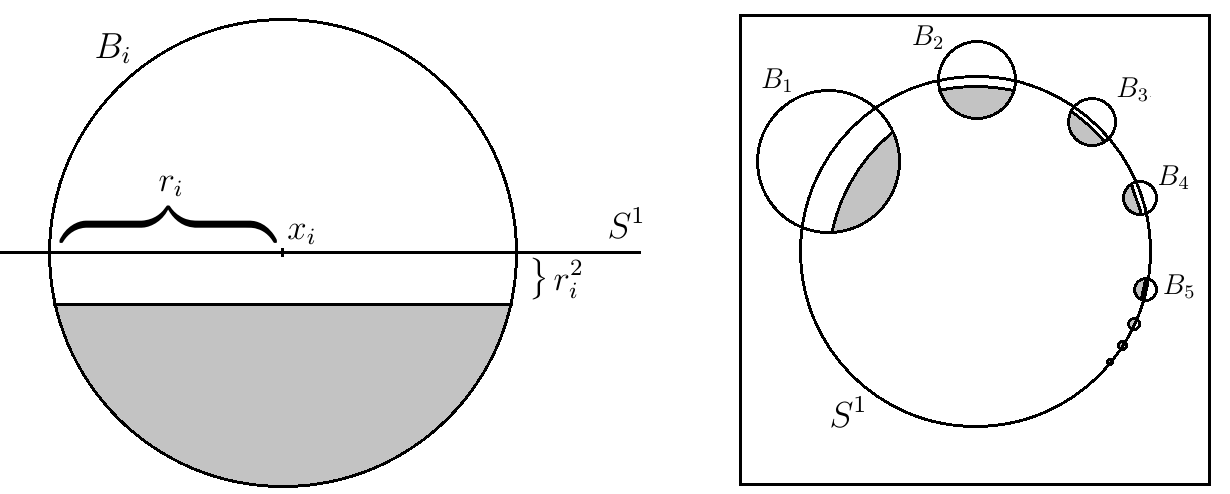
\includegraphics[width=0.9\textwidth]{pics/ch-upper-reg/example.png}
	\caption{Construction of a doubling measure which is not doubling after restricting to the unit ball}
	\label{ch-upper-reg:example}
\end{figure}

We observe  that 2-dimensional Lebesgue measure $\mu$ on $X$ is doubling, but that the restriction of $\mu$ to $B(0,1)$ is not doubling.  It is easy to see that there exists a uniform constant $c>0$ such that for $x \in X$ and $r\in (0,1)$ we have $cr^2 \leq \mu(B(x,r)) \leq \pi r^2$.  It follows that $\mu$ is doubling (with upper regularity dimension 2).  We now consider the restricted measure $\nu = \mu \vert_{B(0,1)}$ and compare the masses of $B(x_i,r_i)$ and $B(x_i,2r_i)$. For large enough $i$ we have $\nu (B(x_i,2r_i)) \ge (\pi (2r_i)^2-\pi r_i^2)/3 = \pi r_i^2$  and $\nu (B(x_i,r_i)) \le 4 r_i^3$. Therefore
\[
\frac{\nu(B(x_i,2r_i))}{\nu(B(x_i,r_i))} \ge \frac{\pi r_i^2}{4r_i^3} =  \frac{\pi}{4r_i} \to \infty
\]
and so  $\nu$ is not doubling.


\subsection{Self-similar measures}\label{ch-upper-reg:sec:self-similarresult}

In this section we compute the regularity dimensions of self-similar measures satisfying the strong separation condition. We emphasise that this separation assumption is natural because self-similar measures not satisfying the strong separation condition are typically not doubling and so have upper regularity dimension equal to $+\infty$. An example of this behaviour is provided below when the strong separation condition is formally defined. 

\nomenclature[IFS1]{IFS}{iterated function system}
\nomenclature[IFS2]{$\mathcal{I}$}{finite index set for an iterated function system}
Let  $\mathcal{I}$ be a finite index set and $\left\{S_i \right\}_{i \in \mathcal{I}}$ be a finite collection of  contraction maps on a compact subset of $\mathbb{R}^d$.  Such a collection is known as an \textit{iterated function system} (IFS).  Also let $\{p_i\}_{i \in \mathcal{I}}$ be a collection of probabilities associated with the maps $\{S_i\}_{i \in \mathcal{I}}$, i.e. we assume that for each $i \in \mathcal{I}$ we have $p_i>0$ and $\sum_{i \in \mathcal{I}} p_i = 1$. There is a  unique non-empty compact set $F$ satisfying 
\[
F=\displaystyle\bigcup_{i\in \mathcal{I}} S_i(F)
\]
and  a unique Borel probability measure $\mu$ satisfying
\[
\mu = \sum_{i \in \mathcal{I}} p_i \mu \circ S_i^{-1}
\]
which is fully supported on $F$, see \cite[Chapter 9]{falconer} and the references therein, notably \cite{hutchinson}. When all of the contractions $S_i$ are similarities, with similarity ratio $c_i \in \left(0,1 \right)$, then $F$ is called a \emph{self-similar set} and $\mu$ is called a \emph{self-similar measure}. These sets are some of the most well studied examples of fractals yet there are many subtleties that we still do not understand, a recent example is \cite{baker}. We refer the reader to \cite{falconer} for a more in depth discussion of IFSs, self-similar sets and measures.

\begin{figure}[h]
	\centering
	\begin{subfigure}{0.3\textwidth}
		\centering
		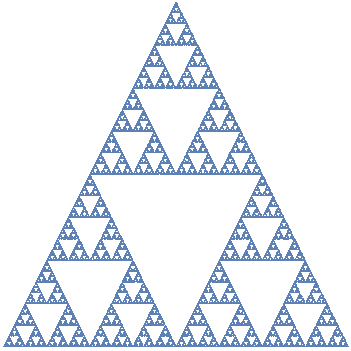
\includegraphics[width=0.85\linewidth]{pics/ch-upper-reg/sierp.png}
	\end{subfigure}%
	\begin{subfigure}{.3\textwidth}
		\centering
		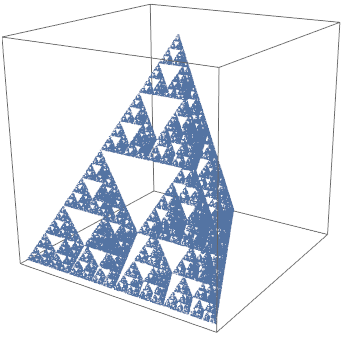
\includegraphics[width=.9\linewidth]{pics/ch-upper-reg/sierptetra.png}
	\end{subfigure}%
	\begin{subfigure}{.3\textwidth}
		\centering
		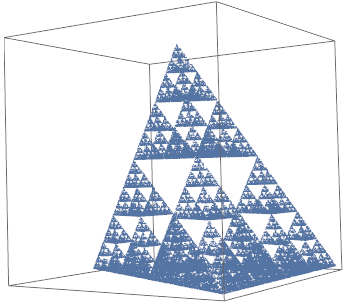
\includegraphics[width=.9\linewidth]{pics/ch-upper-reg/sierptetra2.png}
	\end{subfigure}
	\caption{A self-similar Sierpi\'nski triangle and two perspectives of a self-similar Sierpi\'nski tetrahedron}
	\label{ch-upper-reg:fig:test}
\end{figure}

\nomenclature[SSC]{SSC}{strong separation condition}
We say that the IFS (and associated set $F$ and measure $\mu$) satisfy the \emph{strong separation condition (SSC)} if $S_i(F) \cap S_j(F) = \emptyset$ for all distinct $i,j \in \mathcal{I}$.  This is a natural assumption in the context of the upper regularity dimension. For example, if the defining IFS consists of the maps $x \mapsto x/2$ and $x \mapsto x/2+1/2$, then the SSC is not satisfied and one easily verifies that $\mu$ is doubling if and only if both probabilities are equal to 1/2 and in this case $\mu$ is Ahlfors-David 1-regular (it is Lebesgue measure on the unit interval). On the other hand, when the strong separation condition does not hold, measures can still have positive, even maximal lower regularity dimension; we do not pursue this here and direct the reader towards \cite{hare-troscheit} for further elaboration.  

It is a classical result due to \cite{hutchinson} that the Hausdorff dimension of a self-similar set satisfying the strong separation condition and with contractions $\left\{c_i \right\}_{i\in \lambda}$ is the unique $s$ satisfying $\sum_{i\in \Lambda} c_i^s = 1$. In fact, these sets are incredibly regular so the box, Assouad and lower dimensions are all equal to the Hausdorff dimension. As we weaken the separation condition these numbers start to differ in a number of cases. Studying such cases has seen huge advances recently, as in \cite{hochman2}. The Hausdorff dimension of self-similar measures on self-similar sets satisfying the SSC is known to be $\underline{\dim}_{\textup{H}} \mu = \sum p_i \log p_i / \sum p_i\log c_i$ and these measures are exact dimensional. In this setting the multifractal formalism is satisfied and formulae for the ends of the spectrum can be found in \cite{cawley-mauldin, olsenformalism}.

The regularity dimensions do not behave quite as nicely as one might hope in this setting in the sense that they do not equal the Hausdorff dimension of the measure. However, they do interact pleasantly with the multifractal spectrum of the measure.

\begin{theorem}\label{ch-upper-reg:selfsimilar}
	Let $\mu$ be a self-similar measure as defined above and assume $\mu$ satisfies the SSC.  Then 
	\[
	\urdim \mu = \sup_x \overline{\dim}_{\textup{loc}}(x,\mu) = T(\mu) = \max_{i \in \mathcal{I}} \frac{\log p_i}{\log c_i}
	\]
	and 
	\[
	\lrdim \mu = \inf_x \overline{\dim}_{\textup{loc}}(x,\mu) = t(\mu) = \min_{i \in \mathcal{I}} \frac{\log p_i}{\log c_i}
	\]
\end{theorem}

The Assouad dimension of the self-similar set which supports $\mu$ is generally strictly smaller than the upper regularity dimension of $\mu$ in this setting.  In fact the only case where the geometric dimension and corresponding measure dimension coincide is when  $p_i=c_i^s$, where $s$ is the Hausdorff dimension of the set. In this case $\mu$ is Ahlfors-David $s$-regular and all of the notions of dimension for $F$ and $\mu$ coincide and equal $s$.

\begin{figure}[htb]
    \centering
    \begin{tikzpicture}
\draw (0,0) 
  -- (8,0) 
  -- (4,8) 
  -- cycle;

\draw[black,fill=gray!70] (0,0)
  -- (4/3,8/3) 
  -- (8/3,0) 
  -- cycle;
\draw[black,fill=gray!70] (16/3,0) 
  -- (20/3,8/3) 
  -- (8,0) 
  -- cycle;
\draw[black,fill=gray!70] (4,8)  
  -- (2,4)
  -- (6,4) 
  -- cycle;

\node at (1.25,0.5) {\huge p=1/6};
\node at (6.6,0.5) {\huge p=1/2};
\node at (4,5) {\huge p=1/3};
\end{tikzpicture}
    \caption{First step in the construction of a self-similar set satisfying the SSC and an associated measure}
    \label{fig:ex-self-sim}
\end{figure}



The figure above is the first stage in the construction of a self-similar set in $2$ dimensions with 3 maps $f_1, f_2$ and $f_3$ of respective contraction ratios $1/3$, $1/3$ and $1/2$ and associated probabilities $1/6$, $1/2$ and $1/3$. The attractor $F$ of this IFS satisfies the strong separation condition so the main dimensions all coincide and equal
\[
\dim_\H F = \dim_\textup{B} F = \Assouad F = \lowerdim F \approx 1.17.
\]
The probability vector and the IFS define a self-similar measure $\mu$. The previously discussed dimensions of measures are distinct for this measure with
\[
\underline{\dim}_\H \mu = \frac{4 \log 2 + 3 \log 3}{2 \log 2 + 4 \log 3} \approx 1.05,
\]
\[
\urdim \mu = \frac{\log 6}{\log 3} \approx 1.63
\]
and 
\[
\lrdim \mu = \frac{\log 2}{\log 3} \approx 0.63.
\]


In this section we restricted attention to self-similar sets satisfying the strong separation condition. Whilst certain overlap conditions have been covered in \cite{hare-hare-tros}, and others are already known, it is always of interest to extend to the most general setting possible.
\begin{question}
What are the regularity dimensions of self-similar measures on sets not satisfying the strong separation condition?
\end{question}





\subsection{Self-affine measures}\label{ch-upper-reg:sec:self-affineresults}


In this section we consider an important class of self-affine measures.  Self-affine measures are defined in a similar way to the self-similar measures considered in the previous section, the only difference being that the defining contractions are assumed to be affinities rather than similarities.  In general, such measures are much more difficult to handle due to the fact that different rates of distortion can occur in different directions.  The specific class of self-affine measures we consider are those supported on Bedford-McMullen carpets, see \cite{bedford, mcmullen}, and on the higher dimensional analogues, Bedford-McMullen sponges, see \cite{kenyonperes, sponges}. 

The study of self-affine sets can be broken into two parts: the study of general self-affine sets and specific examples such as Bedford-McMullen carpets. The generic case dates back to Falconer \cite{falconer-affine} where the affinity dimension was first defined. This case has seen a great deal of study recently as in \cite{barany-hochman-rapaport,hochman-rapaport}. On the other hand, studying specific examples has seen a number of different results, including \cite{bedford,mcmullen, lalley-gatzouras, baranski, mackay, Fr}. In particular there is interest in understanding how the special cases, such as carpets, differ from the generic results, see \cite{jurga-morris, morris-sert}. 

\begin{figure}[h]
	\centering
	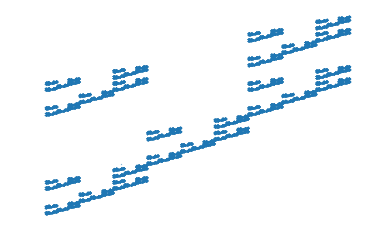
\includegraphics[width=0.8\linewidth]{pics/ch-upper-reg/self-affine-ex.png}
	\label{ch-upper-reg:fig:example-self-affine}
	\caption{An example of a Bedford-McMullen carpet with a 3 by 4 grid and 5 maps}
\end{figure}


Sponges (and measures defined on them) are less commonly studied, but came to prominence recently when they were used by Das and Simmons to provide a counter example to an important and long-standing conjecture in dynamical systems \cite{das-simmons}. In particular, there exists a surprising example of a sponge in $\mathbb{R}^3$ whose Hausdorff dimension cannot be approximated by the Hausdorff dimension of measures invariant under the natural associated dynamical system. This contrasts with the well known result of \cite{kaenmaki-affine} which states that an ergodic invariant measure can be found for typical self-affine sets so that the Hausdorff dimensions coincide.


Let $d \geq 2$ be an integer and fix integers $1<n_1 < n_2 \cdots < n_d$.  Choose a subset $\mathcal{I}$ of $\prod_{l=1}^{d} \left\lbrace 0,\ldots, n_l-1 \right\rbrace$ and for $\textbf{i}=(i_1, \ldots, i_d)\in \mathcal{I} $  let $S_{\textbf{i}} \colon [0,1]^d \rightarrow [0,1]^d$ be defined by
\[
S_{\textbf{i}}(x_1,x_2\ldots, x_d)= \left( \frac{x_1+i_1}{n_1}, \frac{x_2+i_2}{n_2}, \ldots, \frac{x_d+i_d}{n_d} \right) .
\]
Finally, consider the IFS $\{S_i\}_{i \in \mathcal{I}}$  acting on $[0,1]^d$ and let $\{p_i\}_{i \in \mathcal{I}}$ be an associated probability vector as before.  Let $F$ be the associated attractor of this IFS, which is a self-affine set since each of the defining contractions is an affinity, and let $\mu$ be the associated self-affine measure. 



We can now state the separation condition we require, which we note is strictly stronger than the SSC.

\nomenclature[VSSC]{VSSC}{very strong separation condition}
\begin{definition}[VSSC, \cite{sponges}]
	\emph{A self-affine sponge }$F$\emph{ (associated to an index set }$\mathcal{I}$)\emph{ satisfies the }very strong separation condition (VSSC)\emph{ if the following condition  holds. If }$l \in  \left\{1, \ldots, d\right\}$\emph{ and }$(i_1, \ldots, i_d)$, $(j_1 ,\ldots, j_d)\in \mathcal{I}$\emph{ satisfy }$i_1=j_1, \ldots,  i_{l-1}=j_{l-1}$\emph{ and }$i_l \neq j_l$,\emph{ then }$\lvert i_l - j_l \rvert >1$.
\end{definition} 


We assume the self-affine sets studied here satisfy the \emph{very strong separation condition}, which was used by Olsen in \cite{sponges}. Again, this is the natural condition to assume in the context of regularity dimensions because without this assumption the self-affine measures tend not to be doubling, see \cite{doublingcarpets, fraser-howroyd1}. 

\begin{figure}[h]
	\centering
	\begin{subfigure}{0.35\textwidth}
		\centering
		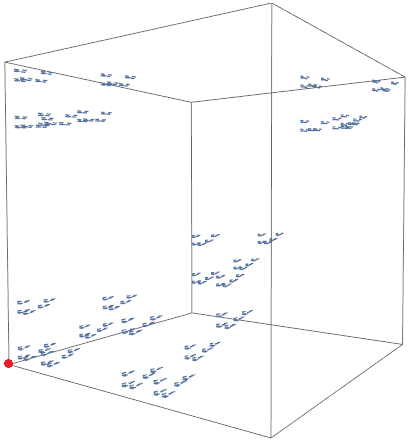
\includegraphics[width=0.8\linewidth]{pics/ch-upper-reg/sponge11.png}
		\label{ch-upper-reg:fig:sub1}
	\end{subfigure}%
	\begin{subfigure}{0.35\textwidth}
		\centering
		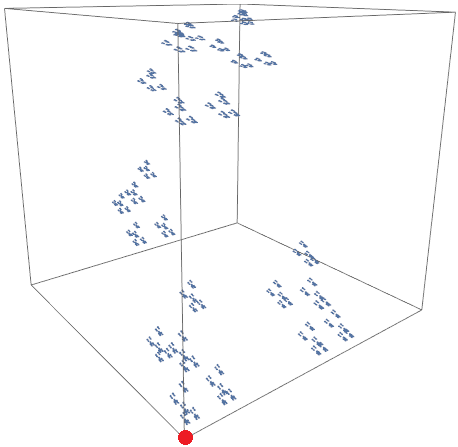
\includegraphics[width=0.85\linewidth]{pics/ch-upper-reg/sponge12.png}
		\label{ch-upper-reg:fig:sub2}
	\end{subfigure}%
	\begin{subfigure}{0.35\textwidth}
		\centering
		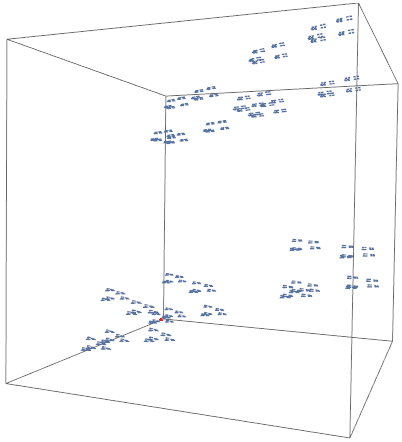
\includegraphics[width=0.85\linewidth]{pics/ch-upper-reg/sponge13.png}
		\label{ch-upper-reg:fig:sub2}
	\end{subfigure}
	\caption{Three perspectives of the self-affine sponge defined by the data: $d=3$,  $n_1=3$, $n_2=4$, $n_3=5$ and $\mathcal{I} = \{ (0,0,0),(0,2,0),(2,1,1)$, $(2,3,4)$, $(0,0,4) \}$. The origin is marked by a red dot to indicate orientation}
\end{figure}


Before we state our result, we need to introduce some more notation.  For $l=1, \dots, d$ and $\textbf{i}=(i_1, \ldots, i_d)\in \mathcal{I} $  let 
\[
p_l(\mathbf{i})=p (i_l \vert i_1, \ldots , i_{l-1})=\frac{\displaystyle\sum_{\substack{\textbf{j}=\left( j_1, \ldots, j_d\right)\in \mathcal{I} \\ j_1=i_1, \ldots, j_{l-1}=i_{l-1}, j_l=i_l}}p_{\textbf{j}}}{\displaystyle\sum_{\substack{\textbf{j}=\left( j_1, \ldots, j_d\right)\in \mathcal{I} \\ j_1=i_1, \ldots, j_{l-1}=i_{l-1}}}p_{\textbf{j}}}
\]
if $(i_1, \ldots, i_l, i_{l+1},\ldots, i_d) \in \mathcal{I}$ for some $i_{l+1},\ldots, i_d$ and $0$ otherwise.  These numbers have a clear interpretation: $p_l(\mathbf{i})$ is the conditional probability that the $l$th digit of an element of $\mathcal{I}$  coincides with the $l$'th digit of $\mathbf{i}$, given that the first $l-1$ coordinates did.  Note that when $l=1$ we are conditioning on the entire space and so the denominator of the above conditional probability is taken to be 1.

\newpage
\begin{theorem}\label{ch-upper-reg:carpet}
	Let $\mu$ be a self-affine measure on a Bedford-McMullen sponge satisfying the VSSC.  Then
	\[
	\urdim \mu =\sum_{l=1}^d \max_{\mathbf{i}\in \mathcal{I}}\frac{-\log p_l(\mathbf{i})}{\log n_l}
	\]
	and 
	\[
	\lrdim \mu =\sum_{l=1}^d \min_{\mathbf{i}\in \mathcal{I}}\frac{-\log p_l(\mathbf{i})}{\log n_l}.
	\]
\end{theorem}

For comparison, we will briefly consider the other notions of dimensions of Bedford-McMullen carpets, restricting to the two dimensional case for ease of notation. Let $N$ be the total number of maps in the IFS and for each column $i\in \left\{0,\ldots, n_1 - 1\right\}$ we define $N_i$ to be the number of maps in that specific column. Finally let $N^0$ to be the total number of non-empty columns. The Hausdorff and box dimensions of Bedford-McMullen carpets $F$ are 
\[
\dim_{\textup{B}} F = \frac{\log N^0}{\log n_1} + \frac{\log N/N^0}{\log n_2}
\]
and 
\[
\dim_{\textup{H}} F = \frac{\log \sum_{i=0}^{n_1 - 1} N_i^{\log n_1 / \log n_2} }{\log n_1}.
\]
The Assouad dimension of these sets was first calculated by Mackay in \cite{mackay}, whilst the lower dimension is due to Fraser in \cite{Fr}, and they are
\[
\Assouad F = \frac{\log N^0}{\log n_1} + \max_{i = 0, \ldots, n_1-1} \frac{\log N_i}{\log n_2}
\]
and 
\[
\lowerdim F = \frac{\log N^0}{\log n_1} + \min_{i = 0, \ldots, n_1-1} \frac{\log \max\{N_i, 1 \}}{\log n_2}.
\]
Note the lower dimension has a $\max\{N_i, 1\}$ in the second fraction, this is to prevent well definededness issues when a column is empty so $N_i \neq 0$.


Formulae for the local dimensions $\sup_x \overline{\dim}_{\text{loc}}(x,\mu), \inf_x \underline{\dim}_{\text{loc}}(x,\mu)$ and spectrum $T(\mu), t(\mu)$ for the self-affine measures $\mu$ we consider in this section can be found in \cite{sponges}, where the notation $\overline{a}, \underline{a}$ and $\overline{A}, \underline{A}$ was used, respectively.


We will now discuss a family of examples designed to demonstrate that all of the notions of dimension we discuss here can be distinct for self-affine measures.  In particular, the upper regularity dimension can be strictly greater than the Assouad dimension, supremum of the upper local dimensions and the `top of the spectrum', $T(\mu)$; similarly for the lower regularity dimension analogues.  This behaviour was \emph{not} seen in the self-similar case.

Let $d=2$, $n_1=3$, $n_2=4$,  $\mathcal{I}=\left\{(0,2),(2,1),(2,3)\right\}$ and $p_{(0,2)}=\epsilon,\, p_{(2,1)}=1-3\epsilon/2$ and $p_{(2,3)}=\epsilon/2$ where we allow $\epsilon$ to vary in the interval $(0,1/2]$.  We write $F$ for the self-affine carpet and $\mu$ for the self-affine measure associated with this data.  Observe that the VSSC is satisfied and so our results apply.  Theorem \ref{ch-upper-reg:carpet} yields
\[
\r = \frac{-\log \epsilon}{\log 3}+ \frac{-\log \frac{\epsilon/2}{1-\epsilon} }{\log 4}
\]
and 
\[
\lrdim \mu = \frac{-\log (1 - \epsilon)}{\log 3}.
\]
Mackay's and Fraser's results give
\[
\dim_{\text{A}} F = \frac{\log 2}{ \log 3} + \frac{ \log 2}{ \log 4} 
\]
and 
\[
\dim_{\text{L}} F = \frac{\log 2}{ \log 3}. 
\]
Olsen gives us
\[
\sup_{x\in F} \overline{\dim}_{\text{loc}}(x,\mu)=\max\left\{ \frac{-\log \epsilon}{\log 3} , \frac{-\log (1-\epsilon)}{\log 3}+\frac{-\log \frac{\epsilon/2}{1-\epsilon} }{\log 4}\right\},
\]
(which has a phase transition at $\epsilon \approx 0.066$),
\[
\inf_{x\in F} \underline{\dim}_{\text{loc}}(x,\mu)=\min\left\{ \frac{-\log \epsilon}{\log 3} , \frac{-\log (1-\epsilon)}{\log 3}+\frac{-\log \frac{1-3\epsilon/2}{1-\epsilon} }{\log 4}\right\},
\]
\[
T(\mu)= \frac{-\log \epsilon }{\log 3} +\frac{\log 2}{\log 4}
\]
and
\[
t(\mu)= \frac{-\log 1- \epsilon }{\log 3} +\frac{\log \frac{2(1-\varepsilon)}{1-3\varepsilon/2} }{\log 4}. 
\]
For $\epsilon \in (0,1/2)$  these quantities are all distinct and for $\epsilon=1/2$ the measure is the `coordinate uniform measure' from \cite{fraser-howroyd1} which has upper regularity dimension precisely equal to the Assouad dimension and lower regularity dimension equal to the lower dimension. This means the larger notions then become all equal and the lower concepts are also all the same, however the lower dimension is strictly less than the Assouad dimension so there is still a gap between them all.



\begin{figure}[H]
	\centering
	\begin{minipage}{.5\textwidth}
		\centering
		\begin{tikzpicture}[scale=0.8]
		\coordinate (O) at (0,0);
		\coordinate (A) at (\Width,0);
		\coordinate (B) at (\Width,\Height);
		\coordinate (C) at (0,\Height);
		\coordinate (C1) at (0,\Height*2/4);
		\coordinate (C2) at (0,\Height*3/4);
		\coordinate (C3) at (\Width/3,\Height*2/4);
		\coordinate (C4) at (\Width/3,\Height*3/4);
		\coordinate (A1) at (\Width*2/3,\Height/4);
		\coordinate (A2) at (\Width*2/3,\Height*2/4);
		\coordinate (A3) at (\Width,\Height/4);
		\coordinate (A4) at (\Width,\Height*2/4);
		\coordinate (D1) at (\Width*2/3,\Height*3/4);
		\coordinate (D2) at (\Width*2/3,\Height);
		\coordinate (D3) at (\Width,\Height*3/4);
		\coordinate (D4) at (\Width,\Height);
		\draw[black] (O) -- (A) -- (B) -- (C) -- cycle;% Bottom Face
		\draw[black,fill=gray!70] (C1) -- (C2) -- (C4) -- (C3) -- cycle;
		\draw (C1) rectangle (C4) node[pos=.5] {\LARGE$\varepsilon$};
		\draw[black,fill=gray!70] (A1) -- (A2) -- (A4) -- (A3) -- cycle;% Bottom Face
		\draw (A1) rectangle (A4) node[pos=.5] {\LARGE$ 1 -  \frac{3\varepsilon}{2}$};
		\draw[black,fill=gray!70] (D1) -- (D2) -- (D4) -- (D3) -- cycle;% Bottom Face
		\draw (D1) rectangle (D4) node[pos=.5] {\LARGE $\frac{\varepsilon}{2}$};
		\end{tikzpicture}
		
	\end{minipage}%
	\begin{minipage}{.5\textwidth}
		\centering
		
		\begin{tikzpicture}[yscale=1]
		\begin{axis}[
		axis lines = left,
		xlabel = $\varepsilon$,
		%xtick={0,0.05,0.1,0.15,0.2,0.25},
		%xticklabels={$0$,,$0.1$,$0.15$,$0.2$,$0.25$}
		]
		%Below the red parabola is defined
		\addplot [
		domain=0:0.5, 
		samples=100, 
		color=red,
		]
		{(-ln(x))/(ln(3)) + (-ln((x/2)/(1-x)))/(ln(4)) };
		\addlegendentry{$\r$}
		
		
		%Here the blue parabloa is defined
		\addplot [
		domain=0:0.5, 
		samples=100, 
		color=blue,
		]
		{(-ln(x))/(ln(3)) + ln(2)/ln(4)};
		\addlegendentry{$T(\mu)$}
		
		
		
		
		%Below the black parabola is defined
		\addplot [
		domain=0.066:0.5, 
		samples=100, 
		color=magenta,
		]
		{- ln((x/2)/(1-x))/ln(4)- ln(1-x)/ln(3)  };
		\addlegendentry{$\sup_x \l$}
		
		
		
		%Below the green parabola is defined
		\addplot [
		domain=0:0.5, 
		samples=100, 
		color=cyan,
		]
		{(ln(2))/(ln(3)) + (ln(2))/(ln(4)) };
		\addlegendentry{$\dim_\text{A} F$}
		
		%Below the green parabola is defined
		\addplot [
		domain=0:0.5, 
		samples=100, 
		color=black,
		]
		{0 };
		
		%Below the black parabola is defined
		\addplot [
		domain=0:0.066, 
		samples=100, 
		color=magenta,
		]
		{  ln(1/x)/ln(3)   };
		
		
		\end{axis}
		\end{tikzpicture}
		
	\end{minipage}
	
	\caption{Left: the affine maps and associated probabilities.  Right: a plot showing the four different `upper dimensions' as $\epsilon$ varies}
	\label{ch-upper-reg:fig:badcarpet}
\end{figure}

As with self-similar measures, we have restricted to self-affine measures satisfying the very strong separation condition. This is natural and indeed necessary for full generality in the upper regularity dimension setting. It seems plausible to make general statements for the lower regularity dimension with weaker separation conditions and perhaps the upper regularity dimension can be computed in specific examples with weaker separation. We could also consider more general self-affine measures such as Lalley-Gatzouras whilst maintaining a strong separation condition, the set theoretic setting has a number of results in this direction which could be examined.

\begin{question}
What can be said about the regularity dimensions of self-affine measures on sets which do not satisfy the VSSC? What are the regularity dimensions of self-affine measures on more general sponges such as Lalley-Gatzouras?
\end{question}


\subsection{Measures on sequences}\label{ch-upper-reg:sec:sequences}

\nomenclature[N]{$\mathbb{N}$}{natural numbers, not including 0}
When one first meets the Assouad and lower dimensions, the first interesting example is often that the set $\left\{1/n \right\}_{n\in \mathbb{N}}$ has Assouad dimension 1, which is strictly larger than the upper and lower box dimensions which are both 1/2, and lower dimension 0. Since this example is so prevalent, we decided to investigate the regularity dimensions of natural families of measures supported on such sets. For simplicity we restrict our examples to countable subsets of $[0,1]$ with one accumulation point at 0 and measures equal to the sum of decaying point masses on the elements of the set. The interplay between the rate of convergence of the points in the set and the rate of decay of the point masses will turn out to be paramount to understanding the dimension of the measure, and to emphasise this we provide exact results for some simple cases where the rates of convergence are either polynomial or exponential.  However, it could be interesting in the future to study  sequences with other decay rates, for example  stretched exponential decay $a^{n^b}$ for $a,b \in (0,1)$, $n \in \mathbb{N}$.

More concretely, consider the set $\left\{ x_n \ : \ n \in \mathbb{N}\right\}$ where  $x_n  \searrow 0$ and the sequence of weights $\left\{ p(n) \ : \ n \in \mathbb{N} \right\}$ where $p(n) \searrow 0$, and $\sum_{n=1}^\infty p(n) < \infty$.  The measure we are interested in is
\[
\mu = \frac{1}{\sum_{n=1}^\infty p(n) } \sum_{n=1}^\infty p(n)\delta_{x_n} 
\]
where $\delta_{x_n} $ is a point mass at $x_n$.

\begin{theorem}\label{ch-upper-reg:sequences}
	Let $\mu$ be as above.
	\begin{enumerate}
		\item Polynomial-polynomial: Let $\lambda > 0$ and $\omega > 1$ and suppose $x_n = n^{-\lambda}$ and $p(n)=n^{-\omega}$.  Then
		\[
		\r \ = \  \max \left\{1, \, \frac{\omega-1}{\lambda}\right\} \  =\  \max \left\{ \textup{supp} (\mu), \, \sup_x \overline{\dim}_{\textrm{loc}}(x,\mu)\right\}.
		\]
		\item Exponential-exponential: Let $\lambda, \omega \in (0,1)$ and suppose $x_n= \lambda^{n}$ and $p(n)=\omega^{n}$.  Then
		\[
		\r \ = \  \frac{\log \omega}{\log \lambda}  \ = \ \sup_x \overline{\dim}_{\textup{loc}}(x,\mu) \ >  \     0 \ = \ \textup{supp} (\mu) .
		\]
		\item Mixed rates: If
		\begin{enumerate}
			\item[(i)] $x_n = n^{-\lambda}$ $(\lambda >0)$ and $p(n)=\omega^{n}$ $(0< \omega < 1)$; or
			\item[(ii)]  $x_n =  \lambda^{n}$ $(0< \lambda < 1)$ and $p(n)=n^{-\omega}$ $(\omega >1)$,
		\end{enumerate}
		then $\mu$ is not doubling, and so  $\r = \infty$.
	\end{enumerate}
\end{theorem}


The above theorem can be summarised by the following table, for suitable values of $\omega$ and $\lambda$:


\begin{table}[h]
	\centering
	\label{ch-upper-reg:sequencetable}
	\begin{tabular}{c|cc}
		$p(n) \setminus x_n$ & $n^{-\lambda}$             & $\lambda^n$                        \\ \hline
		$n^{-\omega}$       & $\max \left\{1,\frac{\omega - 1}{\lambda}\right\}$ & $\infty$\\
		$\omega^n$          & $\infty$                         & $\frac{\log \omega}{\log \lambda}$
	\end{tabular}
\end{table}

The lower dimension of these sequences is always zero and, as the lower regularity dimension is a lower bound to the lower dimension, all of the previously discussed measures $\mu$ satisfy 
\[
\lrdim \mu = 0.
\]
Thus we have examples of doubling measures which are not uniformly perfect. 

Here we see that having different rates for the set and measure always makes the measure non-doubling, investigating different rates of decay as mentioned previously might shed light on this phenomenon and could provide interesting results.

\begin{question}
How does the upper regularity dimension of measures defined on sequences behave for different decay rates such as stretched exponential decay?
\end{question}



\section{Proofs} \label{ch-upper-reg:proof}

We prove Theorems \ref{ch-upper-reg:relationships} and \ref{ch-upper-reg:lower-relationships} in Section \ref{ch-upper-reg:spectrumproof} followed by Theorem \ref{ch-upper-reg:weaktangents} on weak tangents in Section \ref{ch-upper-reg:weaktangentsproof}. Section \ref{ch-upper-reg:self-similar} will concern self-similar measures and will include a proof of Theorem \ref{ch-upper-reg:selfsimilar}. Self-affine measures and the proof of Theorem \ref{ch-upper-reg:carpet} will be dealt with in Section \ref{ch-upper-reg:self-affine} along with some additional notation needed to study Bedford-McMullen sponges. Finally, Theorem \ref{ch-upper-reg:sequences} will be proved in Section \ref{ch-upper-reg:sequenceproof}. Any notation introduced in a subsection should only be used in that proof, but any notation used in Section \ref{ch-upper-reg:results} is assumed throughout the chapter.







\subsection{Proof of Theorem \ref{ch-upper-reg:relationships}: general relationships}\label{ch-upper-reg:spectrumproof}

We start this section with a proof of Theorem \ref{ch-upper-reg:relationships}. Let $\mu$ be a probability measure supported on a compact set $X \subseteq \mathbb{R}^d$. Let $0<s< T(\mu)$,  $\r < t < \infty$ and $q<0$. By definition there exists a  constant  $C \geq 1$ such that for all $x\in X$ and for all $0<r< 1$
\[
\frac{\mu(B(x,1))}{\mu(B(x,r))} \le C \left(\frac{1}{r} \right)^t.
\]
In particular, this guarantees 
\[
\mu(B(x,r))^q \le \frac{1}{C^q}\mu(B(x,1))^q  r^{qt}
\]
and, moreover, 
\[
M_r^q(\mu) \leq c r^{-d}r^{qt}
\]
where $c>0$ is a constant independent of  $r$ and where the $r^{-d}$ term comes from an upper bound on $r$-packings of $X \subseteq \mathbb{R}^d$.  Therefore 
\[
sq > \underline{\tau}(q)   \ge  qt-d
\]
and so $s<t-d/q$ for any $q<0$. By letting $q \rightarrow - \infty$ this yields $s \le t$, which is sufficient to prove that $T(\mu) \leq \r$.

All that remains is to prove that $T(\mu) \geq \l$ for all $x \in X$.  As such, let $x \in X$ and $u>T(\mu)$ which implies that $\underline{\tau}(q)  \geq  uq$ for some $q<0$ which we fix.  Therefore, given $\epsilon>0$, there exists a constant $C_\epsilon>0$ such that
\[
M_r^q(\mu) \leq C_\epsilon r^{uq-\epsilon}
\]
for all $r \in (0,1)$.  Since $\{ B(x,r)\}$ is an $r$-packing of $X$, it follows that
\[
\mu(B(x,r))^q \le M_r^q(\mu) \leq C_\epsilon r^{uq-\epsilon}
\]
and therefore
\[
\mu(B(x,r)) \ge  C_\epsilon^{1/q} r^{u-\epsilon/q}
\]
for all $r\in (0,1)$, which proves that $\l \le u-\epsilon/q$ and since $\epsilon>0$ was arbitrary, this completes the proof of Theorem \ref{ch-upper-reg:relationships}.

This technique can also be used to show Theorem \ref{ch-upper-reg:lower-relationships}. For a measure $\mu$, let $s > t(\mu)$, $0 < t < \lrdim \mu$ and $q > 0$. From the definition of the lower regularity dimension, there exists a constant $C \ge 1$ such that for all $x\in X$ and all $0<r<1$
\[
\frac{\mu(B(x,1))}{\mu(B(x,r))} \ge C \left( \frac{1}{r}\right)^t.
\]
Thus, as $q$ is now positive,
\[
\mu(B(x,r))^q \le C^q \mu(B(x,1))^q r^{tq}
\]
and hence, as before,
\[
M_r^q(\mu) \le cr^{-d}r^{qt}
\]
where $c$ is a constant which does not depend on $r$.

Using $\underline{\tau}(q) = \liminf_{r \rightarrow 0} \frac{\log M_r^q(\mu)}{\log r}$ and the definition of $t(\mu)$ gives
\[
sq > \underline{\tau}(q) \ge qt - d
\]
and so
\[
s> t-\frac{d}{q}.
\]
Letting $q \rightarrow \infty$ gives $s \ge t$ as desired.

To show that $t(\mu) \le \llocal$ for all $x \in X$, let $u < t(\mu)$ so $\underline{\tau}(q) \ge uq$ for some $q > 0$ which is now fixed. Let $ x \in X$ and $\varepsilon > 0$ so there exists a constant $C_{\varepsilon} > 0$ for which
\[
M_r^q(\mu) \le C_\varepsilon r^{uq - \varepsilon}
\]
for all $r \in (0,1)$. Again, using $\{B(x,r) \}$ as an $r$-packing of $X$, shows that
\[
\mu(B(x,r))^q \le C_\varepsilon r^{uq - \varepsilon}
\]
and then, for all $r \in (0,1)$,
\[
\mu(B(x,r)) \le C_\varepsilon^{1/q} r^{u-\varepsilon/q}.
\]
Hence $\llocal \ge u -\varepsilon / q$ and as $\varepsilon$ was arbitrary, this completes the proof.




\subsection{Weak tangent measures} \label{ch-upper-reg:weaktangentsproof}

Let $\mu$ be a locally finite measure on $\mathbb{R}^d$, $\left\{T_k\right\}_{k\in \mathbb{N}}$ a sequence of similarities on $\mathbb{R}^d$ with associated contraction ratios $\{c_k\}_{k\in \mathbb{N}}$, $\left\{p_k\right\}_{k\in \mathbb{N}}$ a sequence of positive renormalising numbers, and $\hat{\mu}$ be a corresponding weak tangent measure of $\mu$, that is a measure on $\mathbb{R}^d$ such that 
\[
p_k \mu \circ T^{-1}_k \rightharpoonup \hat{\mu}
\]
where $\rightharpoonup$ means weak convergence of measures. The Portmanteau Theorem (see \cite[Theorem 1.24]{mattila}) says that this is equivalent to 
\[
\lim_{k\rightarrow \infty} p_k \mu \circ T^{-1}_k (A) =\hat{\mu}(A)
\]
for all $\hat{\mu}$-continuity sets $A$. Recall that  $A\subseteq \mathbb{R}^d$ is a $\hat{\mu}$-continuity set when $\hat{\mu}(\partial A) = 0$ with $\partial A$ being the boundary of $A$. It is a simple exercise to show that for a fixed $x \in \mathbb{R}^d$, all but at most countably many balls $B(x,r)$ are $\hat{\mu}$-continuity sets of $\mathbb{R}^d$. Indeed, assume for a fixed $x \in X$, that there are uncountably many balls of different radii and centre $x$ which are not $\hat{\mu}$-continuity sets. As $\hat{\mu}$ is locally finite, we can write it as a countable sum of finite measures $\hat{\mu}_i$. Since the sets $\partial B(x,r)$ are disjoint for distinct $r$, at most countably many $\partial B(x,r)$ can have positive $\hat{\mu}_i$ measure. Thus at most countably many $\partial B(x,r)$ can have positive $\hat{\mu}$ measure as desired.


We start by proving the upper regularity half of the result. A technical lemma is provided which reduces our calculation of the upper regularity dimension of $\hat \mu$ to the study of balls which are $\hat{\mu}$-continuity sets.

\newpage
\begin{lemma}\label{ch-upper-reg:nu-cont-upper-dim}
	Let $\nu$ be a locally finite measure  on $ \mathbb{R}^d$. Suppose there exist constants $C$ and $s$ such that for all $x\in \textup{supp}(\nu)$ and $0<r<R$ such that $B(x,R)$ and $B(x,r)$ are $\nu$-continuity sets, we have
	\[
	\frac{\nu(B(x,R))}{\nu(B(x,r))} \leq C\left(\frac{R}{r}\right)^{s}.
	\]
	Then $$\overline{\dim}_{\textup{reg}}  \nu \le s.$$
\end{lemma}

\begin{proof}
	Assume 
	\[
	\frac{\nu(B(x,R))}{\nu(B(x,r))} \leq C\left(\frac{R}{r}\right)^{s}
	\]
	holds for all $\nu$-continuity balls. Fix $x  \in \textup{supp}(\nu)$ and let $0<r<R$ be arbitrary. Since there are at most countably many problematic radii, there must exist constants $\theta_1(x,r),\theta_2(x,R)\in[1,2]$ such that $B(x,\theta_1(x,r)^{-1}r)$ and $B(x,\theta_2(x,R) R)$ are $\nu$-continuity balls. Thus
	\[
	\frac{\nu(B(x,R))}{\nu(B(x,r))} \leq \frac{\nu(B(x,\theta_2(x,R)R))}{\nu(B(x,\theta_1(x,r)^{-1}r))} \le   C\left(\frac{\theta_2(x,R)R}{\theta_1(x,r)^{-1}r}\right)^{s} \le 4^s C \left(\frac{R}{r}\right)^{s}
	\]
	and it follows that $\overline{\dim}_{\textup{reg}}  \nu \le s.$
\end{proof}

We now return to proving Theorem \ref{ch-upper-reg:weaktangents}. Let  $x \in \textup{supp}( \hat \mu)$ and $\rho>0$ be such that $B(x,\rho)$ is a $\hat \mu$-continuity set.   Therefore 
\[
\lim_{k\rightarrow \infty} p_k \mu \circ T^{-1}_k (B(x,\rho)) =\hat{\mu}(B(x,\rho)).
\]
Thus, for sufficiently large $k$, 
\begin{equation} \label{ch-upper-reg:estimatee}
\frac{1}{2}p_k \mu \circ T^{-1}_k (B(x,\rho))  \le \hat{\mu}(B(x,\rho))\le 2p_k \mu \circ T^{-1}_k (B(x,\rho)).
\end{equation}
Let $\varepsilon > 0 $ and  $0<r<R$ be such that both $B(x,R)$ and $B(x,r)$ are $\hat \mu$-continuity sets  and  choose $k $ large enough so that  (\ref{ch-upper-reg:estimatee}) holds for $\rho=r$ and $\rho=R$.  In particular,  
\[
\frac{\hat{\mu}(B(x,R))}{\hat{\mu}(B(x,r))} \le 4 \frac{p_k\mu \circ T^{-1}_k (B(x,R))}{p_k \mu \circ T^{-1}_k (B(x,r))}=4\frac{\mu (T^{-1}_k (B(x,R)))}{\mu( T^{-1}_k (B(x,r)))}.
\]
Note that $T_k$ is a similarity of contraction ratio $c_k >0$ and so $T_k^{-1}(B(x,R))= B(T_k^{-1}(x),c_k^{-1}R)$. Thus
\begin{align*}
\frac{\hat{\mu}(B(x,R))}{\hat{\mu}(B(x,r))} &\le 4\frac{\mu (B(T_k^{-1}(x),c_k^{-1}R))}{\mu (B(T_k^{-1}(x),c_k^{-1}r))}.
\end{align*}
Here we wish to apply the definition of the upper regularity dimension of $\mu$, but we cannot do this directly since  $T_k^{-1}(x)$ does not have to be in $\text{supp}(\mu)$. However, we can assume $k$ is large enough (depending on $r$) so that there exists $x'$ in the support of $\mu \circ T_k^{-1}$ which is at distance at most $r/2$ from $x$. Therefore
\[
B(T_k^{-1}(x'),c_k^{-1}r/2)\subset B(T_k^{-1}(x),c_k^{-1}r)
\]
and
\[
B(T_k^{-1}(x),c_k^{-1}R) \subset B(T_k^{-1}(x'), 2c_k^{-1}R)
\]
and $T_k^{-1}(x')$ is in the support of $\mu$.  Thus
\begin{align*}
\frac{\hat{\mu}(B(x,R))}{\hat{\mu}(B(x,r))} &\le 4\frac{\mu (B(T_k^{-1}(x),c_k^{-1}R))}{\mu (B(T_k^{-1}(x),c_k^{-1}r))} \le 4\frac{\mu (B(T_k^{-1}(x'),2c_k^{-1}R))}{\mu (B(T_k^{-1}(x'),c_k^{-1}r/2))} \\
&\le 4C \left(\frac{4c_k^{-1}R}{c_k^{-1}r}\right)^{\r+ \varepsilon} =  4^{1+\r+ \varepsilon}C \left(\frac{R}{r}\right)^{\r+ \varepsilon}
\end{align*}
where $C= C(\varepsilon)>0$ is a uniform constant independent of $x$, $r$ and $R$ which comes from the definition of the upper regularity dimension of $\mu$. Letting $\epsilon \to 0$ proves  $\overline{\dim}_{\textup{reg}} \hat{\mu} \le \r$ as desired.

For the lower dimension, a similar technique also holds. The following lemma is the lower regularity analogue to Lemma \ref{ch-upper-reg:nu-cont-upper-dim}.

\begin{lemma}\label{ch-upper-reg:nu-cont-lower-dim}
	Let $\nu$ be a locally finite measure  on $ \mathbb{R}^d$. Suppose there exist constants $C$ and $s$ such that for all $x\in \textup{supp}(\nu)$ and $0<r<R$ such that $B(x,R)$ and $B(x,r)$ are $\nu$-continuity sets, we have
	\[
	\frac{\nu(B(x,R))}{\nu(B(x,r))} \geq C\left(\frac{R}{r}\right)^{t}.
	\]
	Then $\underline{\dim}_{\textup{reg}}  \nu \ge t.$
\end{lemma}

\begin{proof}
	Assume 
	\[
	\frac{\nu(B(x,R))}{\nu(B(x,r))} \geq C\left(\frac{R}{r}\right)^{t}
	\]
	holds for all $\nu$-continuity balls. Fix $x  \in \textup{supp}(\nu)$ and let $0<r<R$ be arbitrary. As before there must exist constants $\theta_1(x,r),\theta_2(x,R)\in[1,2]$ such that $B(x,\theta_1(x,r)r)$ and $B(x,\theta_2(x,R)^{-1} R)$ are $\nu$-continuity balls. Thus
	\[
	\frac{\nu(B(x,R))}{\nu(B(x,r))} \geq \frac{\nu(B(x,\theta_2(x,R)^{-1}R))}{\nu(B(x,\theta_1(x,r)r))} \ge 4^{-t} C \left(\frac{R}{r}\right)^{t},
	\]
	completing the proof.
\end{proof}

It again suffices to prove Theorem \ref{ch-upper-reg:weaktangents} for $\hat{\mu}$-continuity sets. Let $x \in \textup{supp}( \hat \mu)$, $\varepsilon > 0 $ and  $0<r<R$ be such that both $B(x,R)$ and $B(x,r)$ are $\hat \mu$-continuity sets and choose $k$ large enough so that  (\ref{ch-upper-reg:estimatee}) holds for $\rho=r$ and $\rho=R$. Thus,  
\[
\frac{\hat{\mu}(B(x,R))}{\hat{\mu}(B(x,r))} \ge 4^{-1}\frac{\mu (B(T_k^{-1}(x),c_k^{-1}R))}{\mu (B(T_k^{-1}(x),c_k^{-1}r))}.
\]

As before, $T_k^{-1}(x)$ does not have to be in $\text{supp}(\mu)$ so the definition of the lower regularity dimension can not be applied directly. However, by choosing $k$ large enough (depending on $r$) there exists $x'$ in the support of $\mu \circ T_k^{-1}$ such that
\[
B(T_k^{-1}(x),c_k^{-1}r)\subset B(T_k^{-1}(x'),2c_k^{-1}r)
\]
and
\[
B(T_k^{-1}(x'),c_k^{-1}R/2) \subset B(T_k^{-1}(x), c_k^{-1}R).
\]
Therefore
\begin{align*}
\frac{\hat{\mu}(B(x,R))}{\hat{\mu}(B(x,r))} &\ge  4^{-1}\frac{\mu (B(T_k^{-1}(x'),c_k^{-1}R/2))}{\mu (B(T_k^{-1}(x'),2c_k^{-1}r))} \\
&\ge  (4^{-1})^{1+\lrdim \mu+ \varepsilon}C \left(\frac{R}{r}\right)^{\lrdim \mu + \varepsilon}
\end{align*}
where $C= C(\varepsilon)>0$ is the constant in the definition of the lower regularity dimension of $\mu$. As $\epsilon$ was arbitrary, this proves  $\underline{\dim}_{\textup{reg}} \hat{\mu} \ge \lrdim \mu$ as desired.










\subsection{Proof of Theorem \ref{ch-upper-reg:selfsimilar}: self-similar measures} \label{ch-upper-reg:self-similar}


If $F$ is a self-similar set defined with the IFS $\left\{S_i \right\}_{i\in \mathcal{I}}$, there is a natural correspondence between the geometric fractal $F$ and the symbolic space $\mathcal{I}^{\mathbb{N}}$ (the set of all infinite words over $\mathcal{I}$) via the coding map $\pi \colon \mathcal{I}^{\mathbb{N}} \rightarrow \mathbb{R}^d$ defined by 
\[
\{\pi(i_0,i_1,\ldots) \} =  \bigcap_{n=0}^\infty S_{i_0,\ldots, i_n}(F)
\]
where $S_{i_0,\ldots, i_n} = S_{i_0} \circ \cdots \circ S_{ i_n}$. This technique is useful as the symbolic space is often easier to work with than the Euclidean geometry of the attractor and since $\pi$ provides a natural passage between the two settings we can work in the space that is most helpful whenever desired. 

For $ i_0,i_1,\ldots, i_{n-1} \in \mathcal{I}$ we define a cylinder $[i_0,i_1,\ldots, i_{n-1}] \subseteq \mathcal{I}^\mathbb{N}$, to be the set of all words in $\mathcal{I}^{\mathbb{N}}$ whose first $n$ letters are $i_0,i_1,\ldots, i_{n-1}$. The collection of all level $n$ cylinders corresponds to the  $n$'th level  pre-fractal of the attractor, an approximation of the attractor itself.  It is well-known that $F= \pi(\mathcal{I}^\mathbb{N})$ and the SSC also guarantees that $\pi$ is a bijection so we may interchange the symbolic and geometric spaces.  Also note that  $c_{i_0}\cdots c_{i_{n}}$ is the contraction ratio of the similarity $S_{i_0,\ldots, i_n} $,   $\,\,\pi([i_0,i_1,\ldots, i_{n}] ) = S_{i_0,\ldots, i_n} (F)$ and the $\mu$ measure of $S_{i_0,\ldots, i_n} (F)$  is $p_{i_0}\cdots p_{i_{n}}$.  By rescaling if necessary, we may assume without loss of generality that $\lvert F \rvert=1$. 


We define $\delta$ to be the minimal distance between distinct  sets $S_i(F)$ and $S_j(F)$, that is 
\[
\delta= \min_{i\neq j} \inf_{\substack{x \in S_i(F) \\ y \in S_j(F)}} d(x,y).
\]
The SSC guarantees that $\delta > 0$. Thus the minimal distance between $S_{i_0,\ldots,i_{n-1},i}(F)$ and $S_{i_0,\ldots,i_{n-1},j}(F)$ is at least $c_{i_0}\cdots c_{i_{n-1}} \delta$ for any   $ i_0,i_1,\ldots, i_{n-1} \in \mathcal{I}$ and $i\neq j$.


For $x\in F$ with $\pi(i_0, i_1, \dots)=x$ for a unique $(i_0,i_1,\dots) \in \mathcal{I}^\mathbb{N}$ and small $r>0$, we define the integer $n(x,r)$ to be the largest integer such that $r \le c_{i_0}c_{i_1} \cdots c_{i_{n(x,r)}}$ and so
\[
c_{i_0}c_{i_1} \cdots c_{i_{n(x,r)}+1} < r \le c_{i_0}c_{i_1} \cdots c_{i_{n(x,r)}}.
\]
We also let $m(x,r)$ be the smallest non-negative  integer such that 
$$
\pi([i_0,\ldots, i_{m(x,r)}])\subset B(x,r/2),
$$
and so, in particular,  $p_{i_0}\cdots p_{i_{m(x,r)}} \le \mu (B(x,r))$.  Note that for any $x \in F$, and small $ r>0$,  $c_{i_0} \cdots c_{i_{m(x,r)}} \leq r$. By choosing $m(x,r)$ to be minimal,  $\pi([i_0,\ldots, i_{m(x,r)-1}])$ $\not\subset B(x,r/2)$ and so $c_{i_0} \cdots c_{i_{m(x,r)-1}} \ge r/2$. Using the SSC, we have that for all $x=\pi(i_0,\ldots)$ and  $r>0$, we have $\mu(B(x,\frac{\delta r}{2}))\le p_{i_0}\cdots p_{i_{n(x,r)}}$ where $\delta$ is the separation constant determined by the SSC. This is true since $B(x, \frac{\delta r}{2}) \cap F  \subseteq \pi([i_0,\ldots, i_{n(x,r)}])$.

We are now in a position to prove both parts of Theorem \ref{ch-upper-reg:selfsimilar}. The setup so far is sufficient for both dimension results and the proofs are alike. We start by proving a lower bound to the upper regularity dimension.

Let $x = \pi(\omega_\textup{max})$ where $\omega_\textup{max} \in \mathcal{I}^{\mathbb{N}}$ is an infinite string of the symbol  $i$ which maximises $\log p_i/\log c_i$. It follows that $n(x,r) > \log r / \log {c_i} - 1$ and therefore
\[
\mu(B(x,\delta r/2)) \le p_{i}^{n(x,r)} \leq p_i^{-1} r^{\log p_i/\log c_i}
\]
and it follows that $\overline{\dim}_{\text{loc}}(x,\mu) \geq \log p_i/\log c_i = \colon s$.  Moreover, Theorem \ref{ch-upper-reg:relationships} yields  $ \r  \geq \sup_{x\in F} \overline{\dim}_{\text{loc}}(x,\mu) \ge  s$.  We will now demonstrate the reverse inequality. 





As $F$ satisfies the SSC and $\mu$ is a Bernoulli measure, it is doubling (see \cite{olsenformalism}, for example). Thus recall there exists a constant $C(2/\delta) \geq 1$ depending only on $\delta/2 < 1$ such that $\frac{\mu(B(x, R))}{\mu(B(x,\delta R/2))}\le C(2/\delta)$ for any $x\in F$ and for any $R>0$.  Let $x \in F$ and $0<r<R$ and assume without meaningful loss of generality that $n(x,R) < m(x,r)$. If this were not true, then $R/r$ is bounded above by a uniform constant -- a situation we can safely ignore.  Hence

\begin{align*}
\frac{\mu(B(x,R))}{\mu (B(x,r))}& \le \ C(2/\delta) \frac{\mu(B(x,\delta R/2))}{\mu (B(x,r))}  \\
& \le \ C(2/\delta) \frac{p_{i_0}\cdots p_{i_{n(x,R)}}}{p_{i_0}\cdots p_{i_{m(x,r)}}} \\
& =\  C(2/\delta)  \frac{1}{p_{i_{n(x,R)+1}}} \cdots \frac{1}{p_{i_{m(x,r)}}} \\
& = \ C(2/\delta)  \left(\frac{1}{c_{i_{n(x,R)+1}}}\right)^{\frac{\log p_{i_{n(x,R)+1}}}{\log c_{i_{n(x,R)+1}}} } \cdots \left(\frac{1}{c_{i_{m(x,r)}}}\right)^{\frac{\log p_{i_{m(x,r)}}}{\log c_{i_{m(x,r)} }}} \\
& \le\  C(2/\delta)  \left( \frac{1}{c_{i_{n(x,R)+1}}}\right)^s \cdots \left( \frac{1}{c_{i_{m(x,r)}}}\right)^s \\
%& =\  C(2/\delta)   \left( \frac{c_{(i_0,\ldots, i_{n(x,R)})}}{c_{(i_0,\ldots, i_{m(x,r)})}}\right)^s \\
& = \ C(2/\delta)  \left(\frac{1}{c_{i_{n(x,R)+1}} c_{i_{m(x,r)}}}\right)^s \left( \frac{c_{i_0}c_{i_1} \cdots c_{i_{n(x,R)+1}}}{c_{i_0}c_{i_1} \cdots c_{i_{m(x,r)-1}}}\right)^s \\
& \le \  C(2/\delta)   \left(\frac{2}{c_{\min}^2}\right)^s \left( \frac{R}{r}\right)^s
\end{align*}
where $c_{\min} = \min_{i\in \mathcal{I}}c_i$, is just a constant. The desired upper bound, and the first part of Theorem \ref{ch-upper-reg:selfsimilar}, follows.


To find an upper bound for the lower regularity dimension, choose $x = \pi (\omega_\textup{min})$ with $\omega_\textup{min} \in \mathcal{I}^{\mathbb{N}}$ the infinite string of the repeated symbol $i$ which minimises $\log p_i / \log c_i$. Then $n(x,r) \le  \log r / \log c_i$ and thus
\[
\mu(B(x,\delta r / 2)) \ge r^{\log p_i / \log c_i}.
\]
Hence $\llocal \le \log p_i/\log c_i =: t$ and $\lrdim \mu \le \inf_{x\in F} \llocal \le t$ by Theorem \ref{ch-upper-reg:lower-relationships} as desired.

The lower bound follows in the same way that the upper bound for the upper regularity dimension was found, we summarise this calculation. Note that the measure is still doubling and the previous inequality regarding the doubling constant will be used here, this is simply to make the choice of $n(x,r)$ more natural.

\begin{align*}
\frac{\mu(B(x,R))}{\mu (B(x,r))}& \ge \ C(2/\delta)^{-1} \frac{\mu(B(x,R))}{\mu (B(x,\delta r/2))}  \\
& \ge \ C(2/\delta)^{-1} \frac{p_{i_0}\cdots p_{i_{m(x,R)}}}{p_{i_0}\cdots p_{i_{n(x,r)}}} \\
& = \ C(2/\delta)^{-1}  \left(\frac{1}{c_{i_{m(x,R)+1}}}\right)^{\log p_{i_{m(x,R)+1}}/\log c_{i_{m(x,R)+1}}} \cdots \left(\frac{1}{c_{i_{n(x,r)}}}\right)^{\frac{\log p_{i_{n(x,r)}}}{\log c_{i_{n(x,r)}}} } \\
& \ge\  C(2/\delta)^{-1}  \left( \frac{1}{c_{i_{m(x,R)+1}}}\right)^t \cdots \left( \frac{1}{c_{i_{n(x,r)}}}\right)^t \\
& = \ C(2/\delta)^{-1} \left( \frac{c_{i_0}c_{i_1} \cdots c_{i_{m(x,R)}}}{c_{i_0}c_{i_1} \cdots c_{i_{n(x,r)}}}\right)^t \\
& \ge \  C(2/\delta)^{-1} \left( \frac{c_{i_{m(x,R)}}c_{i_{n(x,r)}}}{2}  \right)^t  \left( \frac{R}{r}\right)^t \ge \  C(2/\delta)^{-1} \left( \frac{c_{\min}^2}{2}  \right)^t  \left( \frac{R}{r}\right)^t
\end{align*}
where $c_{\min}$ is as before, completing the proof.




\subsection{Proof of Theorem \ref{ch-upper-reg:carpet}: self-affine measures} \label{ch-upper-reg:self-affine}



Similar to the previous section, we use the natural correspondence between the self-affine set $F\subseteq \mathbb{R}^d$ and the symbolic space $\mathcal{I}^{\mathbb{N}}$ (the set of all infinite words over $\mathcal{I}$) via the coding map $\pi \colon \mathcal{I}^{\mathbb{N}} \rightarrow \mathbb{R}^d$ defined by 
\[
\{\pi(\textbf{i}_1, \textbf{i}_2, \ldots)\}=  \bigcap_{n=1}^\infty S_{\textbf{i}_1,\ldots, \textbf{i}_n}(F).
\]
where $ S_{\textbf{i}_1,\ldots, \textbf{i}_n} =  S_{\textbf{i}_1} \circ \cdots \circ S_{\textbf{i}_n}$.  Recall that elements of $\mathcal{I}$ have $d$ coordinates so we write $(\mathbf{i}_1,\ldots) = ((i_{1,1},\ldots, i_{1,d}),\ldots) \in \mathcal{I}^{\mathbb{N}} $.

Since the cylinders scale by different amounts in different directions, they do not directly approximate a ball in measure.  For this reason, we introduce \emph{approximate cubes}. For $r\in (0,1]$, choose the unique integers $k_1(r),\ldots,k_d(r)$, greater than or equal to 0, satisfying
\[
\frac{1}{n_l^{k_l(r)+1}}< r \leq \frac{1}{n_l^{k_l(r)}}
\]
for $l=1,\ldots,d$. In particular, 
\[
\frac{-\log r}{\log n_l}-1 < k_l(r) \leq \frac{-\log r}{\log n_l}.
\]
Then the approximate cube $Q(\omega, r)$ of (approximate) side length $r$ determined by $\omega =\left( \textbf{i}_1, \textbf{i}_2 , \ldots \right) =\left( (i_{1,1}, \dots, i_{1,d}), (i_{2,1}, \dots, i_{2,d}) , \ldots \right)    \in \mathcal{I}^{\mathbb{N}}$ is defined by
\begin{align*}
Q(\omega, r)=\big\{ \omega'=\left( \textbf{j}_1, \textbf{j}_2 , \ldots \right)\in \mathcal{I}^{\mathbb{N}} : \forall \, \,  &l=1, \ldots, d \\
&\text{ and } \forall\, \, t= 1, \ldots, k_l(r) \text{ we have } j_{t,l}=i_{t,l} \big\}.
\end{align*}
The geometric analogue is $\pi\left(Q(\omega, r)\right)$, which is contained in
\[ 
\prod_{l=1}^d \left[\frac{i_{1,l}}{n_l}+\cdots+\frac{i_{k_l(r),l}}{n_l^{k_l(r)}} \, , \, \frac{i_{1,l}}{n_l}+\cdots+\frac{i_{k_l(r),l}}{n_l^{k_l(r)}}+\frac{1}{n_l^{k_l(r)}} \right];
\]
a hypercuboid in $\mathbb{R}^d$ aligned with the coordinate axes with side lengths $n_l^{-k_l(r)}$, which are all comparable to $r$ since $ r \leq n_l^{-k_l(r)} < n_l r$.  Thus the measure of a ball can be closely approximated by the measure of an appropriate approximate cube.  This is made precise by the following useful proposition due to Olsen \cite[Proposition 6.2.1]{sponges}.
\begin{proposition}[\cite{sponges}] \label{ch-upper-reg:ballscubes}
	Let $\omega \in \mathcal{I}^{\mathbb{N}}$ and $k \in \mathbb{N}$.
	\begin{enumerate} 
		\item If the VSSC is satisfied, then $B\left( \pi(\omega), 2^{-1}n_1^{-k}\right)\cap F \subseteq \pi \left(Q\left( \omega, n_1^{-k} \right) \right).$ 
		\item  $\pi \left(Q\left( \omega, n_1^{-k} \right) \right) \subseteq B\left( \pi(\omega), (n_1+\dots+n_d)n_1^{-k}\right).$ 
	\end{enumerate}
\end{proposition}

This proposition means, since we assume the VSSC, that a ball of a particular radius contains, and is contained in, an approximate cube of a comparable radius.  Therefore we may replace balls with approximate cubes in the definition of the regularity dimensions, which makes the calculations much easier. This method was used in \cite[Proposition 3.1 and 3.5]{fraser-howroyd1} to calculate the Assouad and lower dimensions of sponges. 

Formally, for any $\omega \in \mathcal{I}^{\mathbb{N}}$ with $x= \pi(\omega) \in F$ and $0<R\le 1$, by Proposition \ref{ch-upper-reg:ballscubes} we see that
\[
\pi(Q(\omega, \frac{R}{n_1(n_1+ \cdots + n_d)}))  \subseteq B(x,R) \subseteq \pi (Q(\omega,2 n_1 R)).
\]
Thus
\[
\frac{\mu \left(\pi \left(Q\left(\omega,\frac{R}{n_1(n_1+ \cdots + n_d)}\right)\right)\right)} {\mu(\pi(Q(\omega,2n_1 r)))} \ \leq \  \frac{\mu(B(x,R))}{\mu(B(x,r))}  \ \leq \ \frac{\mu(\pi(Q(\omega,2n_1 R)))}{\mu \left(\pi \left(Q\left(\omega,\frac{r}{n_1(n_1+ \cdots + n_d)}\right)\right)\right)}
\]
and so to compute $\urdim \mu$ and $\lrdim \mu$ it suffices to consider 
\[
\frac{\mu(\pi(Q(\omega,R)))}{\mu(\pi(Q(\omega,r)))} 
\]
directly. 


Recalling the conditional probabilities $p(i_{l}\vert i_{1},\ldots,i_{l-1})$, defined in Section \ref{ch-upper-reg:sec:self-affineresults}, which give the probability of having $i_{l}$ as the $\text{l}^{\text{th}}$ coordinate given the previous ones, we can write down an explicit formula for the $\mu $ measure of an approximate cube for any $\omega \in \mathcal{I}^{\mathbb{N}}$ and $r \in (0,1)$:
\begin{equation} \label{ch-upper-reg:approxcubemeasure}
\mu(\pi(Q(\omega,r)))=\prod^d_{l=1} \prod_{j=0}^{k_l(r)-1}p_l(\sigma^j\omega)
\end{equation}
where $p_l(\omega)=p(i_{1,l}\vert i_{1,1},\ldots,i_{1,l-1})$ and $\sigma: \mathcal{I}^{\mathbb{N}} \to \mathcal{I}^{\mathbb{N}}$ is the left shift.  This formula follows immediately from the definition of $\mu$ and was first observed by Olsen \cite[Equation 6.2]{sponges}.

With the preliminaries out of the way we are now able to tackle the upper regularity dimension. For $l=1,\ldots, d$, let $p_l^{\text{min}}=\min_{j\in \mathcal{I}} p_l(\mathbf{j})$  and let  $i_l^{\min} \in \mathcal{I}$ be an element achieving this minimum.  If such an element is not unique, it does not matter which we choose. Let $s=\sum_{l=1}^d\frac{-\log p_l^{\text{min}}}{\log n_l}$ be the target dimension. We begin with an upper bound using (\ref{ch-upper-reg:approxcubemeasure}). Let $x = \pi(\omega ) \in F$ and $0< r < R\le 1$ and for convenience we assume without loss of generality that $r < R/ n_d$, which ensures $k_l(R) < k_l(r)$ for all $l$.  We have
\begin{align*}
\frac{\mu(\pi(Q(\omega,R)))}{\mu(\pi(Q(\omega,r)))} \ = \ \frac{\prod_{l=1}^d\left(\prod_{j=0}^{k_l(R)-1}p_l(\sigma^j \omega) \right)}{\prod_{l=1}^d\left(\prod_{j=0}^{k_l(r)-1}p_l(\sigma^j \omega) \right)}  & = \ \frac{1}{\prod_{l=1}^d\left(\prod_{j=k_l(R)}^{k_l(r)-1}p_l(\sigma^j \omega) \right)} \\
& \le\  \prod_{l=1}^d \frac{1}{\prod_{j=k_l(R)}^{k_l(r)-1}p_l^{\text{min}}} \\
& =\  \prod_{l=1}^d\left( \frac{1}{p_l^{\text{min}}}\right)^{k_l(r)-k_l(R)} \\
& \le\  \prod_{l=1}^d \left( \frac{1}{p_l^{\text{min}}}\right)^{-\log r/\log n_l + \log R/\log n_l + 1}  \\
& \le \ p^{-d} \left( \frac{R}{r} \right)^{s}
\end{align*}
where $p = \min_l p_l^{\text{min}}>0$ is a constant. It follows that $\urdim \mu \le s$.

For the lower bound, we aim to find a sequence of points in $F$ and scales $r<R$ for which the ratio of measures will behave like $(R/r)^s$. We have to be a little more careful with the relationship between $R$ and $r$ in this setting though. Again we assume that $r < R/ n_d$, which ensures $k_l(R) < k_l(r)$ for all $l$.  However, for technical reasons we also require $k_l(R) > k_{l+1}(r)$ for all $l = 1, \dots, d-1$.  For this it is sufficient to assume
\[
(n_lR)^{\frac{\log n_{l+1}}{\log n_l}} < r
\]
and fortunately we can choose $r$ satisfying both of these conditions simultaneously.  This is where we use the fact that the $n_l$ are strictly increasing.  Moreover, we can choose a sequence of pairs $(r,R)$ such that $R \to 0$, $R/r \to \infty$ and
\[
(n_lR)^{\frac{\log n_{l+1}}{\log n_l}} < r < R/ n_d.
\]
Let $R,r$ be a pair from this sequence and observe that
\begin{equation} \label{ch-upper-reg:orderingk}
k_d(R)< k_d(r)<k_{d-1}(R)< k_{d-1}(r)< \cdots <k_2(R)<k_2(r)<k_1(R)<k_1(r).
\end{equation}
For fixed $r,R$ as above, let $\omega \in \mathcal{I}^{\mathbb{N}}$ (and so $x = \pi(\omega)$) be chosen such that
\begin{align*} 
\omega&= (i_1,\ldots, i_{k_d(R)}, i_d^{\text{min}},\ldots, i_d^{\text{min}}, i_{k_d(r)+1},\ldots, i_{k_2(R)},\\
&i_2^{\text{min}},\ldots , i_2^{\text{min}}, i_{k_2(r)+1},\ldots, i_{k_1(R)}, i_1^{\text{min}}, \ldots, i_1^{\text{min}}, i_{k_1(r)+1},\ldots),
\end{align*}
where the coordinates not specified as $i_l^{\text{min}}$ (for some $l \in \{1, \dots, d\}$) are arbitrary.  In particular, we insist that the coordinates $i_{k_l(R)+1}, \dots, i_{k_l(r)}$ are all equal to $i_l^{\min}$. Note that we use (\ref{ch-upper-reg:orderingk}) here. We have
\begin{align*}
\frac{\mu(\pi(Q(\omega,R)))}{\mu(\pi(Q(\omega,r)))}  \ = \ \frac{\prod_{l=1}^d\left(\prod_{j=0}^{k_l(R)-1}p_l(\sigma^j \omega) \right)}{\prod_{l=1}^d\left(\prod_{j=0}^{k_l(r)-1}p_l(\sigma^j \omega) \right)} & =\ \frac{1}{\prod_{l=1}^d\left(\prod_{j=k_l(R)}^{k_l(r)-1}p_l(\sigma^j \omega) \right)} \\
& = \ \prod_{l=1}^d\left( \frac{1}{p_l^{\text{min}}}\right)^{k_l(r)-k_l(R)}  \\
& \ge\  \prod_{l=1}^d \left( \frac{1}{p_l^{\text{min}}}\right)^{-\log r/\log n_l -1+ \log R/\log n_l }  \\
& \ge \ p^{d} \left( \frac{R}{r} \right)^{s}
\end{align*}
where $p = \min_l p_l^{\text{min}}>0$ is a constant as before.  Since we can choose a sequence of parameters $x = \pi(\omega)$, $r<R$ satisfying the above with $R/r \to \infty$, it follows that $\urdim \mu \ge s$, completing the proof for the upper regularity dimension.






We proceed in much the same way for the lower regularity dimension, assuming the same preliminary work. For $l=1,\ldots, d$, choose $p_l^{\textup{max}}=\max_{j\in \mathcal{I}} p_l(\mathbf{j})$ and let  $i_l^{\max} \in \mathcal{I}$ be an element achieving this maximum. Again, if multiple options exist, any will suffice. Let $t = \sum_{l=1}^d\frac{-\log p_l^{\text{max}}}{\log n_l}$ be the target dimension. Starting with the lower bound again uses (\ref{ch-upper-reg:approxcubemeasure}). Let $x = \pi(\omega) \in F$ and $0<r<R \le 1$, assuming without loss of generality that $r < R/ n_d$, which guarantees $k_l(R) < k_l(r)$ for all $l$. Then
\begin{align*}
\frac{\mu(\pi(Q(\omega,R)))}{\mu(\pi(Q(\omega,r)))}  & = \ \frac{1}{\prod_{l=1}^d\left(\prod_{j=k_l(R)}^{k_l(r)-1}p_l(\sigma^j \omega) \right)} \\
& \ge\  \prod_{l=1}^d\left( \frac{1}{p_l^{\text{max}}}\right)^{k_l(r)-k_l(R)} \\
& \ge\  \prod_{l=1}^d \left( \frac{1}{p_l^{\text{max}}}\right)^{-\log r/\log n_l -1 + \log R/\log n_l}  \\
& \ge \ p^{d} \left( \frac{R}{r} \right)^{t}
\end{align*}
with $p$ the constant defined previously. It follows that $\lrdim \mu \ge t$.

For the upper bound, the goal is to construct sequences $x$ and $0 < r < R$ for which the expected dimension is attained. Let $0<r<R$ be any reals satisfying the previous restrictions which ensure that $ k_{l+1}(r)< k_l(R) < k_l(r) < k_{l-1}(R)$ holds for all $l$. The assumption that the $n_l$ are strictly increasing still holds in this setting, so such reals exist. Given these $r$ and $R$, choose $\omega \in \mathcal{I}^\mathbb{N}$ so that 
\begin{align*} 
\omega&= (i_1,\ldots, i_{k_d(R)}, i_d^{\text{max}},\ldots, i_d^{\text{max}}, i_{k_d(r)+1},\ldots, i_{k_2(R)},\\
&i_2^{\text{max}},\ldots , i_2^{\text{max}}, i_{k_2(r)+1},\ldots, i_{k_1(R)}, i_1^{\text{max}}, \ldots, i_1^{\text{max}}, i_{k_1(r)+1},\ldots).
\end{align*}
Recall that $i_l^{\text{max}}$ is an element of $\mathcal{I}$ which attains $p_l^{\text{max}}$ and all coordinates not stated as $i_l^{\text{max}}$ are arbitrary. Then, as the $k_l(\cdot)$ are all distinct and well-ordered,
\begin{align*}
\frac{\mu(\pi(Q(\omega,R)))}{\mu(\pi(Q(\omega,r)))}  & =\ \frac{1}{\prod_{l=1}^d\left(\prod_{j=k_l(R)}^{k_l(r)-1}p_l(\sigma^j \omega) \right)} \\
& = \ \prod_{l=1}^d\left( \frac{1}{p_l^{\text{max}}}\right)^{k_l(r)-k_l(R)}  \\
& \le\ \prod_{l=1}^d \left( \frac{1}{p_l^{\text{max}}}\right)^{-\log r/\log n_l + \log R/\log n_l + 1}  \\
& \le \ p^{-d} \left( \frac{R}{r} \right)^{t},
\end{align*}
with $p$ a constant as before. Due to the construction, a sequence of $r$ and $R$ can be chosen to satisfy $R \rightarrow 0$ and $R/r \rightarrow \infty$, simultaneously defining a naturally associated sequence of $x = \pi(\omega)$. These sequences satisfy all of the above and thus $\lrdim \mu \le t$, as desired.




\subsection{Sequences and associated measures}\label{ch-upper-reg:sequenceproof}



We start by explaining our method and then we specialise to the particular cases of  Theorem \ref{ch-upper-reg:sequences} in subsequent subsections.  For convenience, we assume that $x_k \searrow 0$, $x_k-x_{k+1} \searrow 0$ (decreasing gaps) and that $p(k)$ ($k \in \mathbb{N}$) can be extended to a decreasing $L^1$ function $p$ on the whole of $[0,\infty)$.  These conditions are obviously satisfied for the  examples we consider.  Throughout this thesis we write $f(x)=O(g(x))$ to mean $f(x) \le Cg(x)$ for a constant $C$ independent of $x$.

For  $0<r<1$ and $x\in  \textup{supp}(\mu)$, let $\overline{k}(x,r), \underline{k}(x,r)$   be the unique  integers such that $x_{\overline{k}(x,r)+1}<x-r\le x_{\overline{k}(x,r)}$ and  $x_{\underline{k}(x,r)}\le x+r <x_{\underline{k}(x,r)-1}$ where we adopt the convention that $\overline{k}(x,r) = \infty$ when $x-r \le 0$.    Therefore 
$$
\mu(B(x,r))=\frac{1}{\sum_{n=1}^\infty p(n)} \sum_{i=\underline{k}(x,r)}^{\overline{k}(x,r)} p(i).
$$
Of course there is a possibility that $x_{\overline{k}(x,r)}=x$ when $x\neq 0$ and then $\mu(B(x,r))=\mu(\left\{x\right\})$. Thus, given $0<r<R<1$, we will consider three different cases: 
\begin{enumerate}
	\item $x\in \textup{supp}(\mu) \setminus \left\{ 0\right\}$  such that  $x_{\overline{k}(x,r)}=x_{\overline{k}(x,R)}=x$,
	\item $x\in \textup{supp}(\mu) \setminus \left\{ 0\right\}$ such that  $x_{\overline{k}(x,R)}<x_{\overline{k}(x,r)}=x$,
	\item $x\in \textup{supp}(\mu)$ such that  $x_{\overline{k}(x,R)}\le x_{\overline{k}(x,r)}<x$ or $x=0$.
\end{enumerate}
Case 1 is trivial since
\[
\frac{\mu(B(x,R))}{\mu(B(x,r))}=\frac{\mu(\{x\})}{\mu(\{x\})}=1 \leq \left(\frac{R}{r}\right)^0
\]
and so we omit further discussion of it.   We now consider case 3, which is the most important.  Since $p(x)$ is decreasing, we have
$$p(n+1)\le \int_{n}^{n+1}p(x)dx \le p(n)$$
and therefore
\begin{eqnarray*}
	\frac{1}{\sum_{n=1}^\infty p(n)} \int_{\underline{k}(x,r)}^{\overline{k}(x,r)+1} p(x)dx \le  \mu(B(x,r)) &=& \frac{1}{\sum_{n=1}^\infty p(n)}\sum_{i=\underline{k}(x,r)}^{\overline{k}(x,r)} p(i) \\ \\
	&\le& \frac{1}{\sum_{n=1}^\infty p(n)} \int_{\underline{k}(x,r)-1}^{\overline{k}(x,r)} p(x)dx .
\end{eqnarray*}
Hence for any $0<r<R<1$ and any $x\in  \textup{supp}(\mu)$ in case 3 we have
\[
\frac{\mu(B(x,R))}{\mu(B(x,r))} \le \frac{\int_{\underline{k}(x,R)-1}^{\overline{k}(x,R)} p(x)dx}{\int_{\underline{k}(x,r)}^{\overline{k}(x,r)+1} p(x)dx} \le \frac{\int_{\underline{k}(x,R)-1}^{\overline{k}(x,R)} p(x)dx}{\int_{\underline{k}(x,r)}^{\overline{k}(x,r)} p(x)dx}.
\]
To simplify this expression for convenience, we assume that $p(x)$ does not decay faster than exponentially in the sense that there is an $\alpha>0$ such that $p(n)/p(n+1) \le \alpha$ for all $n\in \mathbb{N}$. (This is satisfied for all $p(n)$ we consider.) Then
\begin{align*}
\int_{\underline{k}(x,R)-1}^{\overline{k}(x,R)} p(x)dx &=\int_{\underline{k}(x,R)-1}^{\underline{k}(x,R)} p(x)dx + \int_{\underline{k}(x,R)}^{\overline{k}(x,R)} p(x)dx \\
&\le \alpha^2\int_{\underline{k}(x,R)}^{\underline{k}(x,R)+1} p(x)dx + \int_{\underline{k}(x,R)}^{\overline{k}(x,R)} p(x)dx \\
&\le (\alpha^2+1) \int_{\underline{k}(x,R)}^{\overline{k}(x,R)} p(x)dx 
\end{align*}
Thus in case 3 we have 
\[
\frac{\mu(B(x,R))}{\mu(B(x,r))} \le (\alpha^2+1) \frac{\int_{\underline{k}(x,R)}^{\overline{k}(x,R)} p(x)dx}{\int_{\underline{k}(x,r)}^{\overline{k}(x,r)} p(x)dx}.
\]
In case 2, we get 
\[
\frac{\mu(B(x,R))}{\mu(B(x,r))} \le (\alpha^2+1)  \frac{\int_{\underline{k}(x,R)}^{\overline{k}(x,R)} p(x)dx}{\mu(\{x\})}.
\]
In what follows we will drop the constants $(\alpha^2+1) $ to simplify notation.  We can now apply these bounds to specific sequences and measures to get upper bounds for the upper regularity dimension.  The lower bounds will be provided by Theorem \ref{ch-upper-reg:relationships}.

\subsubsection{Polynomial-polynomial}

Let $p(n)=n^{-\omega}$ and $x_n=n^{-\lambda}$ with $\lambda>0$ and $\omega>1$.  Let $s=\frac{\omega-1}{\lambda}$ be the target dimension and note that
\begin{align*}
(\overline{k}(x,r)+1)^{-\lambda}&<x-r\le \overline{k}(x,r)^{-\lambda} \\
\underline{k}(x,r)^{-\lambda}&\le x+r< (\underline{k}(x,r)-1)^{-\lambda} 
\end{align*}
with $\overline{k}(x,r) = \infty$ if $x-r\le 0$ and thus (for $x > r$)
\begin{align*}
(x-r)^{-1/\lambda}-1 &< \overline{k}(x,r) \le (x-r)^{-1/\lambda} \\
(x+r)^{-1/\lambda} &\le \underline{k}(x,r) < (x+r)^{-1/\lambda}+1.
\end{align*}
We first consider case 3. By our previous calculations, for any $0<r<R<1$ and for any $x\in \textup{supp}(\mu)$ satisfying the conditions required by case 3, we get (up to constants which we ignore)
\begin{eqnarray*}
	\frac{\mu(B(x,R))}{\mu(B(x,r))} \le \frac{\int_{\underline{k}(x,R)}^{\overline{k}(x,R)} x^{-\omega}dx}{\int_{\underline{k}(x,r)}^{\overline{k}(x,r)} x^{-\omega}dx} &\le& \frac{\overline{k}(x,R)^{1-\omega}-\underline{k}(x,R)^{1-\omega}}{\overline{k}(x,r)^{1-\omega}-\underline{k}(x,r)^{1-\omega}} \\ 
	& \le & \frac{(x+R)^{s}-\max\left\{ x-R,0\right\}^{s}}{(x+r)^{s}-\max\left\{x-r,0\right\}^s}.
\end{eqnarray*}



We are interested in the supremum of this upper bound taken over all $x \in [0,1]$.  It turns out that this can be controlled from above by a constant  multiple of the bound evaluated at $x=0$ or $x=R$.  We demonstrate this by repeated application of Taylor's theorem for   $(1+y)^s$ as a function of $y$ close to 0. In particular,   there exist constants $\varepsilon \in (0,1)$ and $C > 0$ (depending only on $s$) such that for any $y \in [-\varepsilon, \varepsilon]$
\[
1 + s y - C y^2 \le (1+y)^s \le 1 + s y + C y^2,
\]
that is $ (1+y)^s = 1 + s y +O( y^2)$.  We may assume $r<\varepsilon^2 R$ and we consider distinct cases (a), (b) and (c).



\noindent (a) Assume $x\in [0,r]$.  In this case the upper bound is decreasing so a bound obtained at $x = 0$ will be a bound for the whole region. When $x=0$ it follows immediately that
\[
\frac{\mu(B(x,R))}{\mu(B(x,r))} \le \left(\frac{R}{r}\right)^s.
\]
\noindent (b) Assume $r < x < R$. 
%not needed?
\begin{comment}
If $x \geq \varepsilon R$,  then
\begin{align*}
\frac{\mu(B(x,R))}{\mu(B(x,r))} &\le \frac{(x+R)^s}{(x+r)^s - (x-r)^s} = \frac{(1+ R/x)^s}{(1+r/x)^s - (1-r/x)^s}\\
&\le \frac{O(1)}{1+sr/x-1+sr/x + O((r/x)^2)}\\ 
&\le O\left(\frac{x}{r} \right) = O\left( \frac{R}{r}\right)    
\end{align*}
which is  the behaviour at $x=R$.  
\end{comment}
If  $x > r/\varepsilon$, then 
\begin{align*}
\frac{\mu(B(x,R))}{\mu(B(x,r))} &\le \frac{(2R/x)^s}{(1+r/x)^s - (1-r/x)^s} \le \frac{(2R/x)^s}{1+sr/x-1+sr/x + O((r/x)^2)}\\ 
&=  (2R/x)^s O(x/r) \le O\left(\left(\frac{R}{r}\right)^{\max\{s,1\}}\right).    
\end{align*}
If $x < r/\varepsilon$, then 
\[
\frac{\mu(B(x,R))}{\mu(B(x,r))} \le \frac{(2R)^s}{(x+r)^s - (x-r)^s} = O\left(\left(\frac{R}{r}\right)^s\right).
\]
The first bound here is controlled from above by the behaviour at  $x=0$ if $s \geq 1$ and $x=R$ if $s <1$ (see below) whilst the second one is simply controlled by the behaviour at $x=0$. 


\noindent (c) Assume  $x \in [R,1]$. If $x \leq R/\varepsilon$, then 
\[
\frac{\mu(B(x,R))}{\mu(B(x,r))} \le \frac{(x+R)^s - (x-R)^s}{(x+r)^s - (x-r)^s} = \frac{(1+R/x)^s - (1-R/x)^s}{(1+r/x)^s - (1-r/x)^s}
\]
and so we use Taylor's Theorem  to obtain
\[
\frac{\mu(B(x,R))}{\mu(B(x,r))} \le \frac{2^s}{1+sr/x + O((r/x)^2)- 1 + sr/x + O((r/x)^2)} \le O\left(\frac{x}{r}\right) = O\left(\frac{R}{r}\right).
\]
If $x > R/\varepsilon$, then  Taylor's theorem can be used on $(1+R/x)^s$ as well, yielding
\begin{align*}
    \frac{\mu(B(x,R))}{\mu(B(x,r))} &\le \frac{(1+R/x)^s - (1-R/x)^s}{(1+r/x)^s - (1-r/x)^s} \\
    &\le \frac{1+sR/x - 1 + sR/x + O((R/x)^2)}{1-sr/x -1 + sr/x + O((r/x)^2)} = O\left(\frac{R}{r}\right)
\end{align*}
as desired. In particular, the bounds attained here are controlled from above by the  behaviour at $x= R$.   This completes the proof in the original case 3.



We now consider case 2, where we have
\begin{align*}
&\frac{\mu(B(x,R))}{\mu(B(x,r))} \le \frac{(x+R)^{s}-\max\left\{x-R,0\right\}^{s}}{x^{\omega/\lambda}}
\end{align*}
up to a constant which we ignore.  This upper bound is decreasing in $x$ and the case 2 assumption forces a lower bound on $x$ in terms of $r$.  Indeed, let $x=n^{-\lambda}$ and note that, since we are in case 2, we have
\[
n^{-\lambda}-  r > (n+1)^{-\lambda}.
\]
It follows that 
\[
r<  n^{-\lambda}- (n+1)^{-\lambda} =  \frac{-1}{\lambda}\int_{n+1}^n z^{-\lambda-1}dz = \frac{1}{\lambda} n^{-\lambda-1}
\]
and rearranging gives
\[
x= n^{-\lambda} > (\lambda r )^{\lambda/(\lambda +1)}.
\]
Therefore, we have
\[
\frac{\mu(B(x,R))}{\mu(B(x,r))} \le   \frac{((\lambda r )^{\lambda/(\lambda +1)}+R)^{s}-\max\left\{(\lambda r )^{\lambda/(\lambda +1)}-R,0\right\}^{s}}{(\lambda r )^{\omega/(\lambda +1)}}
\]
and we split into two further subcases according to which term dominates in the numerator.
\begin{enumerate}
	\item[(i)] If $(\lambda r)^{\lambda/(\lambda+1)}<R$, then
	\[
	\frac{\mu(B(x,R))}{\mu(B(x,r))} \le \frac{(2R)^{s} }{ (\lambda r )^{\omega/(\lambda +1)}}  \le O \left( (R/r)^s \right)
	\]
	provided $s \geq \omega/(\lambda +1)$.  If this is not the case, then simple algebra yields $s < 1$.  This, combined with our assumption  $(\lambda r)^{\lambda/(\lambda+1)}<R$, gives
	\[
	\frac{\mu(B(x,R))}{\mu(B(x,r))} \le \frac{(2R)^{s} }{ (\lambda r )^{\omega/(\lambda +1)}}  \le O \left( R/r \right).
	\]
	\item[(ii)] If $(\lambda r)^{\lambda/(\lambda+1)} \geq R$, then 
	\begin{eqnarray*}
		\frac{\mu(B(x,R))}{\mu(B(x,r))} &\le& \frac{((\lambda r )^{\lambda/(\lambda +1)}+R)^{s}- ((\lambda r )^{\lambda/(\lambda +1)}-R)^{s}}{(\lambda r )^{\omega/(\lambda +1)}} 
	\end{eqnarray*}
	and applying Taylor series estimates in $R/(\lambda r)^{\lambda/(\lambda+1)} \to 0$ similar to above we obtain
	\begin{eqnarray*}
		\frac{\mu(B(x,R))}{\mu(B(x,r))} &\le& \frac{(\lambda r)^{s\lambda/(\lambda+1)}}{(\lambda r )^{\omega/(\lambda +1)}} \, O \left( R/(\lambda r)^{\lambda/(\lambda+1)} \right) \le O \left( R/r \right).
	\end{eqnarray*}
\end{enumerate}


Combining the above estimates gives $\r\le\max \{s,1\}$.  Finally, note that $\overline{\dim}_{\text{loc}}(x,\mu)=0$ when $x\neq 0$, since such $x$ are atoms.  However, when $x=0$, the above estimates  immediately give $\overline{\dim}_{\text{loc}}(0,\mu)= s$ and it is well-known that $\text{supp}(\mu) = 1$, which, combined with Theorem \ref{ch-upper-reg:relationships}, completes the proof of the `polynomial-polynomial' part of Theorem \ref{ch-upper-reg:sequences}.


\subsubsection{Exponential-exponential}



Let $ x_n = \lambda^{n} $ with associated probabilities $p(n)=\omega^{n}$, where $\lambda, \omega \in (0,1)$ and let $s=\frac{\log \omega}{\log \lambda}$ be the target dimension. The situation is much simpler than in the `polynomial-polynomial' case due to the exponential convergence allowing rougher estimates.  In particular, for any $x \in [0,1]$ and $0<r<R$ with $(r/R)$ sufficiently small, we have
\begin{eqnarray*}
	\frac{\mu(B(x,R))}{\mu(B(x,r))} \le \frac{\int_{\underline{k}(x,R)-1}^{\overline{k}(x,R)} \omega^x dx}{\int_{\underline{k}(x,r)}^{\overline{k}(x,r)+1} \omega^x dx} = \frac{\omega^{\underline{k}(x,R)-1} - \omega^{\overline{k}(x,R)} }{\omega^{\underline{k}(x,r)}-\omega^{\overline{k}(x,r)+1}  }  &\le&  \frac{\omega^{\underline{k}(x,R)-1}   }{\omega^{\underline{k}(x,r)}(1-\omega)  } \\ \\
	&  \le& \frac{1}{\omega^2(1-\omega)} \frac{(x+R)^s}{(x+r)^s} \\ \\
	&  \le& O\left(  (R/r)^s \right)
\end{eqnarray*}
which proves that $\r \leq s$.  Again,  it is clear that $\overline{\dim}_{\text{loc}}(x,\mu)=0$ when $x\neq 0$ but $\overline{\dim}_{\text{loc}}(0,\mu)= s$ and it is well-known that $\text{supp}(\mu) = 0$, which resolves the `exponential-exponential' part of  Theorem \ref{ch-upper-reg:sequences}.






\subsubsection{Mixed rates}


We first consider the case where  $x_n=n^{-\lambda}$ with associated probability vector $p(n)=\omega^n$, where $\lambda>0$ and $\omega\in(0,1)$.  Choosing  $x=0$ and $r=R/2$ we get
\[
\frac{\mu(B(0,R))}{\mu(B(0,R/2))}   \geq  \frac{\int_{\underline{k}(x,R)}^\infty \omega^x dx}{\int_{\underline{k}(x,R/2)-1}^\infty \omega^x dx} \geq   \omega^{R^{-1/\lambda}-(R/2)^{-1/\lambda}} \to \infty
\]
as $R \to 0$, which proves that $\mu$ is not doubling, as required.
\\ \\
We now consider the opposite case, where $x_n=\lambda^{n}$ with associated probability vector $p(n)=n^{-\omega}$, where $\lambda\in (0,1)$ and $\omega > 1$. Curiously, and in contrast to the previous case,  the measure is `very doubling' at 0. As such, to demonstrate that the measure is non-doubling, we choose $x=R$ and $r=R/2$.  Our previous estimates yield that for sufficiently small $R>0$ and up to a constant that we ignore
\begin{eqnarray*}
	\frac{\mu(B(R,R))}{\mu(B(R,R/2))}   \geq  \frac{(-\log 2R)^{1-\omega}}{(-\log \frac{3R}{2})^{1-\omega} - (-\log\frac{R}{2} )^{1-\omega}}   \to \infty
\end{eqnarray*}
as $R \to 0$, proving that  $\mu$ is non-doubling.

\chapter{Quantifying doubling and uniform perfectness}
\label{chap:quantifying}


\section{Introduction}
\label{sec:intro-quantifying}


The goal of this chapter is to quantify how doubling a measure is via the upper regularity dimension and uniformly perfect through the lower regularity dimension. This will start with a simple relationship between these notions which will then help understand a classic technical result regarding the measure of balls. The notion of quasisymmetric invariant will then be studied by calculating bounds for the regularity dimensions of pushforward measures under such maps with respect to the dimensions of the original measures. Finally a relation between the lower regularity dimension and a regularity of measures property recently introduced in Diophantine approximation will be discussed. This leads to a more quantitative statement of a recent theorem in the Diophantine approximation on Kleinian groups.





\section{Results}\label{ch-quantifying:sec:results}

We start by establishing some well known facts and introducing our results. Section \ref{ch-quantifying:sec:equivalence} will study the link between the regularity dimensions and the doubling constants and constants of uniform perfectness and these notions will help to quantify a well known technical proposition in Section \ref{ch-quantifying:sec:quantifying}. Quasisymmetric homeomorphisms will be introduced in Section \ref{ch-quantifying:sec:quasi} with the goal of understanding how the regularity dimensions can be changed under the action of such maps. Finally Section \ref{ch-quantifying:sec:diophantine} will be spent discussing a result from Diophantine approximation and relating it to our work on the regularity dimensions.


\subsection{Quantifying doubling and uniform perfectness}\label{ch-quantifying:sec:equivalence}

Recall from the introduction, that a measure is doubling if and only if it has finite upper regularity dimension; similarly for uniformly perfect and the lower regularity dimension. Repeatedly, we have stated that this means the regularity dimensions quantify doubling and uniform perfectness without further elaboration. This can be formalised so the upper regularity dimension of a doubling measure can be stated explicitly as a function of the doubling constants; similarly for the lower regularity dimension with respect to the constants of uniform perfectness when this dimension is stictly positive. 

\begin{theorem}\label{ch-quantifying:equivalence}
Let $\mu$ be a doubling measure fully supported on a metric space $X$ with doubling constants $C(\theta)$, then $$\urdim \mu = \inf_{\theta > 1}\frac{\log C(\theta)}{\log \theta}.$$ Similarly if $\mu$ is a uniformly perfect measure with constants of uniform perfectness $K(\theta)$ then $$\lrdim \mu = \sup_{\theta > 1} \frac{\log K(\theta)}{\log \theta}.$$
\end{theorem}


Unfortunately these formulae are supremums and infimums and so the regularity dimensions are not even always attained for any $\theta$. This means we cannot restate results regarding the doubling constants with solely the upper regularity dimension.

We consider two examples which illustrate this result. First let $F$ be the middle third Cantor set and $\mu$ the self-similar measure fully supported on $F$ with associated probability vector $\left\{ 1/4, 1/2 \right\}$, as introduced in the previous chapter. We know the upper regularity dimension is $\log 4 / \log 3$ whilst the lower regularity dimension is $\log(4/3) / \log 3$. Start by just considering balls centred on the origin, of radius $3^{-k}$ for some $k \in \mathbb{N}$ and with $\theta = 3^{l}$ for any $l \in \mathbb{N}$. Due to the structure of $F$ it is clear that 
\[
\mu(B(0, 3^{-k})) = 4^{l} \mu(B(0, 3^{-(k+l)}))
\]
and so $C(3^{l}) \ge 4^l$. Thus 
\[
\urdim \mu = \log 4 / \log 3 \ge \frac{\log C(3^{l})}{ \log 3^{l}} \ge \frac{ \log 4^l}{\log 3^l} =  \log 4 / \log 3
\]
and so for any $l \in \mathbb{N}$, $C(3^l) = (3^l)^{\urdim \mu}$. Similarly by focusing on balls centred on 1 we can see that $K(3^l) = (3^l)^{\lrdim \mu}$. For $\theta \neq 3^l$ we do not obtain precise values for $C(\theta)$ or $K(\theta)$ using this method, it would be interesting to see if renewal theory or some other technique could be used to achieve precise formulae for a greater range of $\theta$. 

On the other hand, self-affine measures $\mu$ supported on Bedford-McMullen carpets $F$ provide examples where the natural balls do not provide $C(\theta)$ for which the upper regularity dimension is attained for finite $\theta$. In particular, fix $R> 0$ and $\theta > 1$ then consider $x =\pi(\omega) \in F$ where $\omega$ is the word used in the lower bound in the proof of the upper regularity half of Theorem \ref{ch-upper-reg:carpet} from the previous chapter. Following the proof of that theorem we see that
\[
\frac{\mu(B(x,R))}{\mu(B(x,R/\theta))} \le c p^d \theta^{\urdim \mu}
\]
where $c$ is some constant which comes from passing between balls and approximate cubes so depends on the structure of $F$ and $p$ is a constant depending on the probability vector associated with $\mu$. Thus $C(\theta) \ge cp^d \theta^{\urdim \mu}$ and when $cp^d \neq 1$ this provides examples where $C(\theta)$ is either not equal to $\theta^{\urdim \mu}$ for finite $\theta$ or there is a sequence of points and radii for which $C(\theta) = \theta^{\urdim \mu}$ but these are not the expected sequences and it is not clear where this would occur. A similar argument can be made for the lower regularity dimension and $K(\theta)$ in this setting; further exploration of these ideas in the self-affine case and for more general sets would be interesting.


\subsection{Quantifying an example of Heinonen}\label{ch-quantifying:sec:quantifying}


When studying doubling measures a technical proposition is often employed to truly benefit from the regularity of these measures. Simply put, a doubling measure on a uniformly perfect space is also a uniformly perfect measure. This implies the following important bounds. Say $\mu$ is a doubling measure on a uniformly perfect, bounded space $X$, then there exists constants $0< \lambda_1, \lambda_2 < \infty$ and $0 < t \le s < \infty$ such that for any $x \in X$ and $0 < r$
\[
\lambda_1 r^s \le \mu(B(X,r)) \le \lambda_2 r^t.
\]
It is not clear where this was first stated, but the standard reference \cite{heinonen} provides this result as an example (\cite[Exercise 13.1]{heinonen}) without a proof. 

This result opens a number of questions. Notably, how close to zero can the lower regularity dimension be in this setting? Clearly the lower regularity dimension of $\mu$ must depend on the lower dimension of $X$, since the lower dimension is an upper bound, see \cite{bylund}. But in principle this does not bound the lower regularity dimension from below in any meaningful way. 

One could ask if there exists a fixed uniformly perfect space and a sequence of doubling measures on that space which all have the same upper regularity dimension but whose lower regularity dimensions can be made as small as possible. A cursory check of some standard examples such as self-similar sets and measures implies this might not be feasible, Theorem \ref{ch-upper-reg:selfsimilar} of the previous chapter is helpful here. Heuristically, by keeping the upper regularity dimensions of self-similar measures fixed with a goal of decreasing the lower regularity dimension, we must increase a probability from the associated probability vector which is not the minimum of the vector. As this is a probability vector, the sum of the elements is always one so any increase must be accompanied by a decrease in at least one other element. If the lower regularity dimension is to approach zero in the limit a probability must tend towards one and thus all other probabilities must be lowered towards zero. This will inevitably increase the upper regularity dimension after some number of steps, breaking the assumption.

\begin{figure}[h]
    \centering
    \begin{tikzpicture}[scale=0.8]
		\coordinate (O) at (0,0);
		\coordinate (A) at (\Width,0);
		\coordinate (B) at (\Width,\Height);
		\coordinate (C) at (0,\Height);
		\coordinate (C1) at (0,\Height*2/4);
		\coordinate (C2) at (0,\Height*3/4);
		\coordinate (C3) at (\Width/3,\Height*2/4);
		\coordinate (C4) at (\Width/3,\Height*3/4);
		\coordinate (A1) at (\Width*2/3,\Height/4);
		\coordinate (A2) at (\Width*2/3,\Height*2/4);
		\coordinate (A3) at (\Width,\Height/4);
		\coordinate (A4) at (\Width,\Height*2/4);
		\coordinate (D1) at (\Width*2/3,\Height*3/4);
		\coordinate (D2) at (\Width*2/3,\Height);
		\coordinate (D3) at (\Width,\Height*3/4);
		\coordinate (D4) at (\Width,\Height);
		\draw[black] (O) -- (A) -- (B) -- (C) -- cycle;% Bottom Face
		\draw[black,fill=gray!70] (C1) -- (C2) -- (C4) -- (C3) -- cycle;
		\draw (C1) rectangle (C4) node[pos=.5] {\LARGE$\varepsilon$};
		\draw[black,fill=gray!70] (A1) -- (A2) -- (A4) -- (A3) -- cycle;% Bottom Face
		\draw (A1) rectangle (A4) node[pos=.5] {\LARGE$ 1 -  2\varepsilon$};
		\draw[black,fill=gray!70] (D1) -- (D2) -- (D4) -- (D3) -- cycle;% Bottom Face
		\draw (D1) rectangle (D4) node[pos=.5] {\LARGE $\varepsilon$};
\end{tikzpicture}
    \caption{Example of a self-affine set and measure which also demonstrates how the increase in probability of the lower right map will force the remaining probabilities to zero.}
    \label{fig:pathos-ex}
\end{figure}


This lends credibility to the conjecture that the example of Heinonen implies a lower bound to the lower regularity dimension as a function of the upper regularity dimension. We wish to quantitatively show this result. More precisely, given a measure $\mu$ of fixed upper regularity dimension $s$ on a space $X$ of fixed lower dimension $l$, can we bound the lower regularity dimension of $\mu$ as a function of $s$ and $l$? The following does not quite answer this question as it returns a function of the doubling and uniform perfectness constants. However, as we will discuss, this is closer to the desired solution than it appears.

\begin{proposition}\label{ch-quantifying:result-heinonen}
	If $X$ is uniformly perfect and $\mu$ is a doubling, fully supported measure on $X$ then $\mu$ is uniformly perfect. In particular if $X$ is $K$-uniformly perfect and $\mu$ doubling with doubling constants $C(\theta)$ then  
	$$\lrdim \mu \ge \frac{\ln(1-C(8K)^{-1})}{\ln(4K)} .$$  
\end{proposition}


Combining this result with Theorem \ref{ch-quantifying:equivalence}, it follows that a doubling measure on a uniformly perfect space must have lower regularity dimension bounded below by a function of the upper regularity dimension and the constant of uniform perfectness. However, as eluded to previously, Theorem \ref{ch-quantifying:equivalence} is concerned only with the infimum over all $\theta$ and the formula in Proposition 2.1 relies on a specific $C(\theta)$, we cannot, in general, find an exact formula linking the lower regularity dimension and the upper regularity dimension in our setting.


We finish this section with a brief discussion of the sharpness of this result. Assuming positive lower dimension of the space is required here as it is simple to construct spaces of zero lower dimension but finite Assouad dimension. In such a setting there must exist a measure of upper regularity dimension close to the Assouad dimension of the space and so doubling. But any measure on this space cannot be uniformly perfect as the lower regularity dimension is a lower bound to the lower dimension. A trivial such example would be the set of points $\left\{ 1/n : n \in \mathbb{N} \right\}$ with the Euclidean metric. This set is know to have zero lower dimension but full Assouad dimension; doubling measures on this space were explicitly constructed in the previous chapter. On the other hand we can take an atomic measure on a self-similar set, this measure is neither doubling nor uniformly perfect. Thus the obtained bound is justified in demanding both the doubling constants of $\mu$ and the constant of uniform perfectness of the set.

There are many examples of uniformly perfect measures, even on doubling spaces, that are not doubling so we cannot interchange the two notions and obtain an analogous result.  For instance, one can take a self-similar set with overlaps, this is a doubling space. Numerous uniformly perfect measures exist on such a space and are not doubling, as can be seen in \cite{hare-troscheit}. Thus a uniformly perfect measure on a space of positive, finite lower and Assouad dimension need not be doubling.




\subsection{Regularity dimensions under quasisymmetric homeomorphisms}\label{ch-quantifying:sec:quasi}


Quasisymmetric homeomorphisms are a generalisation of bi-Lipschitz maps, preserving relative sizes but not necessarily global size which were first introduced in \cite{ahlfors-beurling, tukia-vaisala}. In the Euclidean setting quasisymmetric homeomorphisms are equivalent to the often studied quasiconformal homeomorphisms. Recall that $d_X(\cdot,\cdot)$ denotes the metric on the space $X$, tracking which space we are working in will be important in this section. A homeomorphism $f\colon X \rightarrow Y$ is an \textit{$\eta$-quasisymmetric homeomorphism} if there is a homeomorphism $\eta \colon [0,\infty) \rightarrow [0,\infty)$ such that 
\[
d_X( x , a ) \le t \, d_X( x , b )
\]
implies 
\[
d_Y( f(x) , f(a) ) \le \eta(t) \, d_Y ( f(x) , f(b) )
\]
for all $x,a,b \in X$ and for all $t>0$.
\textcolor{red}{add more intro shit here?}

Equivalently there exists a homeomorphism $\eta$ as above such that 
\[
\frac{d_Y(f(x),f(y))}{d_Y(f(x),f(z))} \le \eta \left(\frac{d_X(x,y)}{d_X(x,z)} \right)
\]
for any distinct points $x,y,z \in X$. Here $\eta$ is not unique for a given quasisymmetric homeomorphism. 


A property of particular interest to us is that doubling and uniform perfectness of spaces are quasisymmetric invariants. This can be quantified, so there are bounds on the Assouad and lower dimensions of images of spaces under quasisymmetric embeddings. Formally for a set $F$ and a quasisymmetric map $f$ we have
\[
\alpha \Assouad F \le \Assouad f(F) \le \frac{1}{\alpha} \Assouad F
\]
where $\alpha$ is some constants intrinsic to the map $f$ which will be introduced shortly. The classic book \cite{heinonen} contains further details and many other interesting properties of these maps that we will not touch upon in this thesis.

We wish to know if the same holds for doubling and uniformly perfect measures. In particular we will study \textit{pushforward measures} under quasisymmetric homeomorphisms. Given a measure $\mu$ on a space $X$ and $f$ a map from $X$ to some space $Y$, the pushforward measure of $\mu$ under $f$ is denoted $f_*\mu$ and is defined by
\nomenclature[.]{$f_*\mu$}{pushforward measure of $\mu$ under map $f$}
\[
f_*\mu (A) = \mu(f^{-1}(A))
\]
for any measureable subset $A$ of $Y$, where $f^{-1}(A) = \left\{x \in X \colon f(x) \in A \right\}$. 

To avoid having trivial upper and lower regularity dimensions of $\mu$ it is reasonable to assume that $X$ is doubling and uniformly perfect. This then lets us employ the following theorem. 

\begin{theorem}[{\cite[Theorem 13.11]{heinonen}}]
	A quasisymmetric homeomorphism $f$ of a uniformly perfect space $X$ is $\eta$-quasisymmetric with $\eta$ of the form
	\[
	\eta(t) = c_\eta \max\left\{t^\alpha, t^{1/\alpha}\right\},
	\]
	where $c_\eta \ge 1 $ and $\alpha \in (0,1]$ depend only on $f$ and $X$.
\end{theorem}
For clarity we will often write $\eta_{\alpha}$ to indicate the homeomorphism $\eta$ associated with the constant $\alpha$ as described here. Section 3 of \cite{tukia-vaisala} proves this result and explicitly calculates $\alpha$. 

For such quasisymmetric homeomorphisms we see that doubling and uniform perfectness of measures are also invariants, mirroring the geometric setting.

\begin{theorem}\label{ch-quantifying:quaisymm-thm}
	Let $X$ be a uniformly perfect space and $\mu$ be doubling on $X$. When $f$ is an $\eta_\alpha$-quasisymmetric homeomorphism the following bounds hold
	\[
	\alpha \, \urdim \mu \le \urdim f_{*}\mu \le \urdim \mu/\alpha
	\]
	and 
	\[
	\alpha \, \lrdim \mu \le \lrdim f_{*}\mu \le \lrdim \mu/\alpha
	\]
	where $f_{*}\mu = \mu \circ f^{-1}$ is the pushforward of $\mu$.
\end{theorem}



\subsection{Uniformly perfect and weakly absolutely $\alpha$-decaying measures}\label{ch-quantifying:sec:diophantine}

A property that has appeared recently in Diophantine approximation is the notion of weakly absolutely $\alpha$-decaying. This was first introduced in \cite{beres-sanju-al} following the previous uses of friendly measures by \cite{friendly} and quasi-decaying measures by \cite{decaying1, decaying2}. A measure $\mu$ is weakly absolutely $\alpha$-decaying for some $\alpha > 0$ when there exists constants $C, R_0 >0$ such that for all $\varepsilon > 0$
\[
\mu(B(x,\varepsilon R)) \le C \varepsilon^{\alpha} \mu(B(x,R))
\]
for all $x \in X$ and $R<R_0$.

This property has some resemblance to the ideas of doubling and uniformly perfect measures. We show the following.
\begin{proposition}\label{ch-quantifying:equiv-diophantine}
	If a measure $\mu$ has positive lower regularity dimension then 
	\[
	\lrdim \mu = \sup\left\{\alpha \colon \mu \text{ is weakly absolutely $\alpha$-decaying}\right\}.
	\]
\end{proposition}

This result actually leads to an equivalent but hopefully more applicable statement of Theorem 2 in \cite{beres-sanju-al}. Their theorem concerns the size of the set of points which well approximate a given point $y$ with respect to some function $\psi$ for limit sets of Kleinian groups $\Lambda$. In the Euclidean setting, one usually considers the Lebesgue measure of this set. However when working on different sets other measures must be considered that somewhat mirror the regularity of Lebesgue measure. This leads to the notion of $\alpha$-decaying. Without further elaborating on the definitions we state both the old and new versions of the theorem. \textcolor{red}{add more detail here meebs }

\begin{theorem}[{\cite[Theorem 2]{beres-sanju-al}}]
	Let $G$ be a nonelementary, geometrically finite Kleinian group and let $y$ be a parabolic fixed point of $G$, if there are any, and a hyperbolic fixed point otherwise. Fix $\alpha > 0$, and let $K$ be a compact subset of $\Lambda$ equipped with a weakly absolutely $\alpha$-decaying meausre $\mu$. Then
	\[
	\mu(K\cap W_y(\psi)) = 0 \quad if \quad \sum_{r=1}^\infty r^{\alpha-1} \psi(r)^{\alpha} < \infty.
	\]
\end{theorem}

\begin{theorem}
	Assume $G$ and $y$ are as above. Let $K$ be a compact subset of $\Lambda$ with lower dimension equal to $s > 0$. For any $0 < \alpha < s$, if there exists a weakly absolutely $\alpha$-decaying measure $\mu$ on $K$, then
	\[
	\mu(K\cap W_y(\psi)) = 0 \quad if \quad \sum_{r=1}^\infty r^{\alpha-1} \psi(r)^{\alpha} < \infty.
	\]
	In particular, if  $\sum_{r=1}^\infty r^{s-1} \psi(r)^{s} < \infty$ then any weakly absolutely $\alpha$-decaying measure on $K$ is such that $\mu(K\cap W_y(\psi)) = 0$. One can also find a sequence of weakly absolutely $\alpha_n$-decaying measures on $K$ such that $\alpha_n \rightarrow s$. 
\end{theorem}

An advantage of writing the theorem with respect to the lower dimension of the limit set is that the lower dimension of limit sets were calculated in \cite{fraser2}. Therefore, given a limit set, we can quickly check if there will be measures that are weakly absolutely $\alpha$-decaying such that the sum in the theorem converges for the given $\alpha$. In \cite{fraser2}, Fraser also calculated the regularity dimensions of Patterson-Sullivan measures, providing us with explicit measures that could be used in the theorem, as the upper and lower regularity dimensions of Patterson-Sullivan measures are strictly positive and finite. 

Theorem 7 follows from Proposition 5 and Theorem 6. As such we do not provide a proof here, for the interested reader the proof of Theorem 6 in \cite{beres-sanju-al} is very accessible.
\textcolor{red}{should I actually go through this here?}

Weakly absolutely decaying measures were the correct measures to consider in the setting of limit sets of Kleinian groups whereas friendly measures were used in the context of subsets of Euclidean space. It would be a natural extension to study the links between friendly measures and the regularity dimensions, especially given that one of the conditions for a measure to be friendly is that it is doubling.  



\section{Proofs}


This proof section will be broken into several subsections that are mostly independent of each other but the notation will remain consistent throughout. In Section \ref{ch-upper-reg:doublingproof} we cover the ideas found in Section \ref{ch-quantifying:sec:equivalence} relating the regularity dimensions with their associted regularity constants. In Section \ref{ch-quantifying:sec:proof-heinonen} we show Proposition \ref{ch-quantifying:result-heinonen}. Section \ref{ch-quantifying:proof-quasi} is dedicated to the study of quasisymmetric homemorphisms and Theorem \ref{ch-quantifying:quaisymm-thm}. Finally in Section \ref{ch-quantifying:diophantine-proof} a short proof of Proposition \ref{ch-quantifying:equiv-diophantine} is provided.


\subsection{Proof of equivalence of doubling and finite upper regularity dimension} \label{ch-upper-reg:doublingproof}


We start by proving the link between the upper regularity dimension and the doubling constants. Recall the notion of doubling implies the existence of constants $C(\theta)$; we wish to pick the optimal constant. Given $\theta > 1$ let
\[
C(\theta) = \sup \left\{ \frac{\mu(B(x,R))}{\mu(B(x,R/\theta))} \ : \ x \in \text{supp}(\mu), R>0 \right\} \geq 1.
\]

Assume that a measure $\mu$ on a space $X$ is doubling and let $\theta > 1$.  Therefore, for all $x \in \text{supp}(\mu)$ and $R>0$
\[
\frac{\mu(B(x,R))}{\mu(B(x,R/\theta))} \le C(\theta).
\]
Fix  $0< r < R$ and  define $k$ to be the unique integer such that $R\theta^{-k} > r \ge R\theta^{-k-1}$. Then by telescoping we obtain
\[
\frac{\mu(B(x,R))}{\mu(B(x,r))} = \frac{\mu(B(x,R))}{\mu(B(x,\theta^{-1} R))} \times \frac{\mu(B(x,\theta^{-1} R))}{\mu(B(x,\theta^{-2} R))} \times\cdots \times \frac{\mu(B(x,\theta^{-k} R))}{\mu(B(x,\theta^{-k-1}R))} \times \frac{\mu(B(x,\theta^{-k-1}R))}{\mu(B(x,r))}.
\]
Thus 
\[
\frac{\mu(B(x,R))}{\mu(B(x,r))} \le C(\theta)^{k+1}  \frac{\mu(B(x,\theta^{-k-1}R))}{\mu(B(x,r))} \le C(\theta)^{\log(R/r) / \log \theta+1} = C(\theta) \left(\frac{R}{r} \right)^{\log C(\theta) / \log \theta}
\]
and hence $\r \leq \log C(\theta) / \log \theta < \infty$, giving the upper bound.


To obtain a lower bound on the upper regularity dimension, it suffices to find, for $s = \inf\frac{\log C(\theta)}{\log \theta}$, a sequence of $x\in X$ and $0<r<R$, with $R/r \rightarrow \infty$, such that 
\[
\frac{\mu(B(x,R))}{\mu(B(x,r))} \ge \left(\frac{R}{r}\right)^s.
\]
	
	
From the definition of doubling we know that $\mu(B(x,\theta r) ) \le C(\theta) \mu(B(x,r))$ for all $x,r, \theta$. Fixing $\theta$ we pick $C(\theta)$ to be reasonably sharp in the sense that there exists at least one pair of $x,r$ such that $\mu(B(x,\theta r) ) \ge \frac{1}{2}C(\theta) \mu(B(x,r))$. Choosing $C(\theta)$ to be optimal as above would ensure this for instance.
	
Recall $s = \inf_{\theta > 1}\frac{\log C(\theta)}{\log \theta}$. To choose our sequence of $x,r$ and $R$ we simply pick any sequence of increasing $\theta$. Then from our choice of $C(\theta)$, the pair $x$ and $r$ are the pair obtained above. $R$ is then fixed by $R = \theta r$. Finally, due to the choice of $s$,
\[
\frac{\mu(B(x,R))}{\mu(B(x,r))} \ge \frac{1}{2} C(\theta)  \ge \frac{1}{2}\theta^s = \frac{1}{2}\left(\frac{R}{r} \right)^s,
\]
completing the proof for the upper regularity dimension.
	

The lower regularity dimension result follows similarly. Recall a measure $\mu$ is uniformly perfect if and only if it has positive lower regularity dimension and thus there exists constants $K(\theta)$ for all $\theta > 1$ such that 
\[
K(\theta) =  \inf \left\{ \frac{\mu(B(x,R))}{\mu(B(x,R/\theta))} \ : \ x \in \text{supp}(\mu), R>0 \right\} \geq 1.
\]

For all $x \in \text{supp}(\mu)$ and $0<r<R$, fix $k$ to be the unique integer such that $R \theta^{-k} > r \ge R \theta^{-k-1}$. Then by the above argument
\[
\frac{\mu(B(x,R))}{\mu(B(x,r))} = \frac{\mu(B(x,R))}{\mu(B(x,\theta^{-1}R))} \times \cdots \times \frac{\mu(B(x,\theta^{-k}R))}{\mu(B(x,r))} \ge K(\theta)^k \frac{\mu(B(x,\theta^{-k}R))}{\mu(B(x,r))} \ge K(\theta)^k.
\]
Approximating $k$ yields
\[
\frac{\mu(B(x,R))}{\mu(B(x,r))} \ge K(\theta)^{\log(R/r)\log(\theta) - 1} = K(\theta)^{-1} \left(\frac{R}{r}\right)^{\log K(\theta)/ \log \theta}
\]
so $\lrdim \mu \ge \log K(\theta) / \log \theta$ for any $\theta > 1$ as desired. 

For the upper bound, we again find a sequence of $x\in X$ and $0<r<R$ which will attain the dimension. Recall, for a fixed $\theta > 1$, we can choose $x,r$ such that $\mu(B(x,\theta r)) \le \frac{1}{2}K(\theta)\mu(B(x,r))$. 

Let $t = \sup_{\theta > 1} \frac{\log K(\theta)}{\log \theta}$ and choose any sequence of strictly increasing $\theta > 1$. This gives us sequences of $x,r$ for which $K(\theta)$ satisfies the above condition and then pick $R = \theta r$. Thus
\[
\frac{\mu(B(x,R))}{\mu(B(x,r))} \le \frac{1}{2} K(\theta) \le \frac{1}{2} \theta^t = \frac{1}{2} \left(\frac{R}{r} \right)^t
\]
completing the proof.



\subsection{Quantifying an example of Heinonen}\label{ch-quantifying:sec:proof-heinonen}



Let $X$ and $\mu$ be as in the statement of the proposition with constant of uniform perfectness $K$ and doubling constants $C(\theta)$. We will rework the proof found in \cite[lemma 3.1]{anti1}, paying careful attention to the constants in play. Note there is another proof in \cite[Lemma 4.5]{eino-pablo} which could lead to different bounds, but we do not pursue this here.
	
To start, a technical result is required. Proposition B.4.7, in \cite{gromov}, states that in our setting there exists a constant $a \in (0,1)$ such that 
\[
\mu(B(x,aR)) \le (1-a) \mu(B(x,R))
\]
for any $x,R$. We start by determining $a$ as a function of our known constants. 
	
For any $x\in X$ and $R>0$, as $X$ is uniformly perfect, there exists $y \in X$ such that $$\frac{R}{2K} \le d(x,y) \le \frac{R}{2}.$$ This choice of $y$ ensures that $B(x,\frac{R}{4K}) \cap B(y,\frac{R}{4K}) = \emptyset $ and $B(x,\frac{R}{4K}) \cup B(y,\frac{R}{4K}) \subseteq B(x,R)$. Thus
\begin{align*}
\mu(B(x,R/(4K))) &\le \mu(B(x,R)) - \mu(B(y, R/(4K)))\\
& \le \mu(B(x,R)) - \frac{1}{C(8K)}\mu(B(y,2R)) \\
& \le \mu(B(x,R)) - \frac{1}{C(8K)}\mu(B(x,R)) \\
& = (1-C(8K)^{-1}) \mu(B(x,R)).
\end{align*}
Recall $C(8K)$ is the doubling constant of $\mu$ where $\theta = 8K$. By iterating this construction we obtain
\[
\mu(B(x,R/(4K)^n)) \le (1-C(8K)^{-1})^n \mu(B(x,R))
\]
for any $n\in \mathbb{N}$, as desired.
	
Returning to the actual question, fix $x\in X$, $0 < r < R$ and choose $n\in \mathbb{N}$ such that $(4K)^{-n-1}R < r \le (4K)^{-n}R$ so that $B(x,r) \subseteq B(x,R/(4K)^{n})$. Then
\begin{align*}
\frac{\mu(B(x,R))}{\mu(B(x,r))} \ge& \frac{\mu(B(x,R))}{(1-C(8K)^{-1})^n\mu(B(x,R))} \\
& \ge (1-C(8K)^{-1})^{\frac{-\ln(R/r)}{\ln(4K)} + 1}\\
& = (1-C(8K)^{-1})\left(\frac{R}{r}\right)^{\frac{\ln(1-C(8K)^{-1})}{\ln(4K)}}
\end{align*}
as desired.
	
Note that in the proof of \cite{gromov} one should use the optimal doubling and uniform perfectness constants to obtain the best bound possible, however the result itself is likely not sharp.






\subsection{Regularity dimensions under quasisymmetric homeomorphism}\label{ch-quantifying:proof-quasi}


Whilst Theorem 13.11 of \cite{heinonen} is the key ingredient in the proof of Theorem \ref{ch-quantifying:quaisymm-thm}, the following proposition which can also be found in \cite{heinonen} is also required.

\begin{proposition}[{\cite[Proposition 10.6]{heinonen}}]
	When a quasisymmetric homeomorphism $f\colon X \rightarrow Y$ is $\eta$-quasisymmetric, its inverse $f^{-1}$ is an $\eta'$-quasisymmetric homeomorphism with $\eta'$ given by  $\eta'(t) = 1/\eta^{-1}(1/t)$ for $t>0$.
\end{proposition}

It is then clear that a quasisymmetric homeomorphism $f$ on a uniformly perfect space is associated with a homeomorphism $\eta(t) = c_\eta\max\left\{t^\alpha, t^{1/\alpha}\right\}$ and $f^{-1}$ is also a quasisymmetric homeomorphism associated with the function $1/\eta^{-1}(1/t) \le c_\eta^{1/\alpha} \max\left\{t^\alpha, t^{1/\alpha} \right\}$. Note that the homeomorphism $\eta'(t) = c_\eta^{1/\alpha} \max\left\{t^\alpha, t^{1/\alpha} \right\}$ is not exactly $1/\eta^{-1}(1/t)$, but, as it is a upper bound to the desired function, $f^{-1}$ will be an $\eta'$-quasisymmetric homeomorphism.



We start by stating some technical calculations which will be relevant for both the upper and lower regularity dimensions. Let $y\in Y$ and $0<r<R$. Since $Y$ is uniformly perfect, we can find $z_1,z_2$ such that $z_1\in B_Y(y,KR) \setminus B_Y(y,R)$ and $z_2 \in B_Y(y,Kr) \setminus B_Y(y,r)$. Without loss of generality, choose $ r < 2R $ so that $d_Y(y,z_1) > d_Y(y,z_2)$,  this will be required to use the exact formula for $\eta$.
	
	
Choose any point $a \in B_Y(y,R)$. From our choice of $z_1$, it is clearthat$d_Y( y , a ) \le d_Y(y , z_1)$. Thus, as $f$ is quasisymmetric $d_X( f^{-1}(y) , f^{-1}(a) ) \le \eta(1)  d_X(f^{-1}(y) , f^{-1}(z_1) $, and so 
	\[
f^{-1}(B_Y(y,R)) \subseteq B_X(f^{-1}(y),\eta(1)d_X(f^{-1}(y), f^{-1}(z_1)).
	\]
Similarly, choosing $a \in B_Y(y,R) \setminus B_Y(y,R/K)$, we have $d_Y( y , a ) \ge d_Y( y , z_1 )/K^2$ and so $$d_X( f^{-1}(y) , f^{-1}(a) ) \ge \eta^{-1}(K^2) d_X( f^{-1}(y) , f^{-1}(z_1) ).$$
Hence 
\[
f^{-1}(B_Y(y,R)) \supseteq B_X(f^{-1}(y),\eta^{-1}(K^2)d_X(f^{-1}(y),f^{-1}(z_1))).
\]
Similar statements clearly hold for $r$ with $z_2$. 

We can now prove the upper bound for the upper regularity dimension. For any $\varepsilon > 0$,
\begin{align*}
\frac{\mu(f^{-1}(B_Y(y,R)))}{\mu(f^{-1}(B_Y(y,r)))} &\le \frac{\mu(B_X(f^{-1}(y),\eta(1)d_X(f^{-1}(y), f^{-1}(z_1)) ))}{\mu(B_X(f^{-1}(y),\eta^{-1}(K^2)d_X(f^{-1}(y),f^{-1}(z_2)) ))} \\
& \le C_{\varepsilon}\left( \frac{\eta(1)d_X(f^{-1}(y),f^{-1}(z_1))}{\eta^{-1}(K^2)d_X(f^{-1}(y),f^{-1}(z_2))}\right)^{\urdim \mu + \varepsilon} \\
& \le C_{\varepsilon}\left(c_\eta^{\alpha} \eta(1)/\eta^{-1}(K^2)\right)^{\urdim \mu + \varepsilon} \left(\frac{d_Y(y,z_1)}{d_Y(y,z_2)} \right)^{(\urdim \mu + \varepsilon)  / \alpha} \\
& \le C_{\varepsilon}\left(c_\eta^{\alpha} \eta(1)/\eta^{-1}(K^2)\right)^{\urdim \mu + \varepsilon} \left(\frac{KR}{r} \right)^{(\urdim \mu +\varepsilon)/ \alpha},
\end{align*}
where $C_{\varepsilon}$ is the constant from the definition of the upper regularity dimension of $\mu$ with respect to $\varepsilon$. As $\varepsilon$ is arbitrarily chosen this completes the upper bound, that is $\urdim f_*\mu \le \urdim \mu / \alpha$.
	
For the lower bound recall $f^{-1}$ is an $\eta'$-quasisymmetric homeomorphism where $\eta'$ is of the form $\eta_\alpha$ with the same $\alpha$ as in $\eta$. Thus the measure $f^{-1}_* (f_*\mu)$ is the pushforward measure of $f_*\mu$ under the quasisymmetric map $f^{-1}$. Therefore the above bound also holds for this new measure and so $\urdim f^{-1}_* (f_*\mu) \le \urdim f_* \mu / \alpha$. Since $f$ is a homeomorphism this yields $\alpha\, \urdim \mu \le \urdim f_* \mu$ as expected. 


The lower regularity dimension can be shown in much the same way, we start with the lower bound. Let $\varepsilon > 0$,
\begin{align*}
\frac{\mu(f^{-1}(B_Y(y,R)))}{\mu(f^{-1}(B_Y(y,r)))} &\ge \frac{\mu(B_X(f^{-1}(y),\eta^{-1}(K^2)d_X(f^{-1}(y),f^{-1}(z_1)) ))}{\mu(B_X(f^{-1}(y),\eta(1)d_X(f^{-1}(y), f^{-1}(z_2)) ))} \\
& \ge D_{\varepsilon}\left( \frac{\eta^{-1}(K^2)d_X(f^{-1}(y),f^{-1}(z_1))}{\eta(1)d_X(f^{-1}(y),f^{-1}(z_2))}\right)^{\lrdim \mu - \varepsilon} \\
& \ge D_{\varepsilon}\left(\frac{1}{c_\eta^{\alpha}} \eta^{-1}(K^2)/\eta(1)\right)^{\lrdim \mu - \varepsilon} \left(\frac{d_Y(y,z_1)}{d_Y(y,z_2)} \right)^{\alpha \,(\lrdim \mu - \varepsilon)} \\
& \ge D_{\varepsilon}\left(\frac{1}{c_\eta^{\alpha}} \eta^{-1}(K^2)/\eta(1)\right)^{\lrdim \mu - \varepsilon} \left(\frac{R}{K r} \right)^{\alpha \,(\lrdim \mu - \varepsilon)},
\end{align*}
where $D_\varepsilon$ is the constant stemming from the lower regularity dimension of $\mu$ as a function of $\varepsilon$. Letting $\varepsilon$ tend to zero finishes the proof of $\lrdim f_*\mu \ge \alpha \, \lrdim \mu$.

For the upper bound, we again argue that $f_*^{-1}(f_*\mu) = \mu$ giving $\lrdim f_*^{-1}(f_* \mu) \ge \alpha \, \lrdim f_*^{-1} \mu$. Hence, $\lrdim f_* \mu \le \lrdim \mu / \alpha$.











\subsection{Uniformly perfect and weakly absolutely $\alpha$-decaying measures}\label{ch-quantifying:diophantine-proof}



	If $\mu$ is weakly absolutely $\alpha$-decaying then $\mu(B(x,\varepsilon R)) \le C \varepsilon^{\alpha} \mu(B(x,R))$ for any $x\in X$ and $\varepsilon, R >0$. Thus
	\[
	\frac{\mu(B(x,R))}{\mu(B(x,\varepsilon R))} \ge \frac{1}{C} \left(\frac{R}{\varepsilon R} \right)^{\alpha}
	\]
	and so $\lrdim \mu \ge \alpha$.
	
	For the other direction, assume $\lrdim \mu = t$. Then for any $\delta > 0$, there exists $C' > 0$ such that for all $x\in X$ and $R>r>0$ 
	\begin{align*}
	\frac{\mu(B(x,R))}{\mu(B(x,r))} &\ge C' \left( \frac{R}{r}\right)^{t - \delta}.
	\end{align*}
	Given $\varepsilon \in (0,1)$ and $R > 0$, choose $r = \varepsilon R$. Inserting this value of $r$ into the above yields 
	\[\mu(B(x,R)) \ge C' \left(\frac{R}{\varepsilon R}\right)^{t-\delta} \mu(B(x,\varepsilon R)).
	\]
	Hence
	\[
	\mu(B(x,\varepsilon R)) \le \frac{1}{C'} \varepsilon^{t - \delta} \mu(B(x,R))  
	\]
	and so $\mu$ is $(t-\delta)$-decaying.





\chapter{Graphs of Brownian motion}
\label{chap:graphs}

\section{Introduction}
\label{sec:intro-brownian}

Studying the dimension of various random processes has been of interest for quite some time. In this chapter we will consider the Assouad and lower dimensions of graphs of certain random processes, notably L\'evy processes and functions defined by stochastic integrals. Then the regularity dimensions of pushforward measures onto graphs of L\'evy processes will be computed for doubling measures defined on the unit interval. 

In particular we will see that pushforwards of doubling maps in this setting are almost surely not doubling. This contrasts with the previous results on quasisymmetric homeomorphisms which conserved doubling. This will also provide a nice example of a uniformly perfect and doubling space with a non uniformly perfect and non doubling measure fully supported on that same space.

\section{L\'evy processes}
\label{sec:levy-process}


\emph{L\'{e}vy processes} $X(t)$ were first introduced by Paul L\'evy in 1934 \cite{levy} and are defined to be the stochastic processes satisfying:
\begin{itemize}
	\item[1]: $X(0)=0$ almost surely.
	\item[2]: For all $t,h>0$, $X(t+h)-X(t)$ is equal to $X(h)$ in distribution (stationary increments).
	\item[3]: For all $0<t_1<t_2<...<t_k$ the random variables $X(t_i)-X(t_{i-1})$ are independent (independence of increments).
	\item[4]: For all $t>0$ $\lim_{h\to 0} X(t+h)-X(t)=0$ in probability (continuity).
\end{itemize}

We can construct $X(t)$ such that it is almost surely right continuous with left limits (denoted c\`adl\`ag). Such processes are standard tools in many areas of modern mathematics and its applications. A common example of a L\'evy process is the \emph{Wiener process} (or Brownian motion) where property 2 (stationary increments) is replaced by Gaussian increments, so $X(t+h)-X(t)$ is normally distributed with mean 0 and variance $h$. One can similarly define $d$-dimensional Brownian motion by considering the vector-valued stochastic process $(W_1,\ldots, W_d)$ where the $W_i$ are independent Weiner processes. 


\begin{figure}[htbp]
	\centering
	\begin{subfigure}{0.3\textwidth}
		\centering
		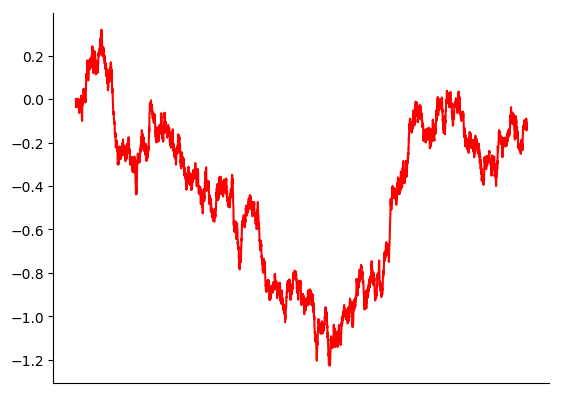
\includegraphics[width=0.85\linewidth]{2-brownianr.png}
	\end{subfigure}%
	\begin{subfigure}{.3\textwidth}
		\centering
		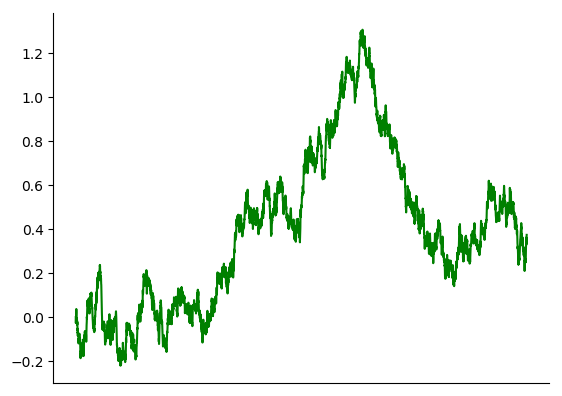
\includegraphics[width=.9\linewidth]{2-browniang.png}
	\end{subfigure}%
	\begin{subfigure}{.3\textwidth}
		\centering
		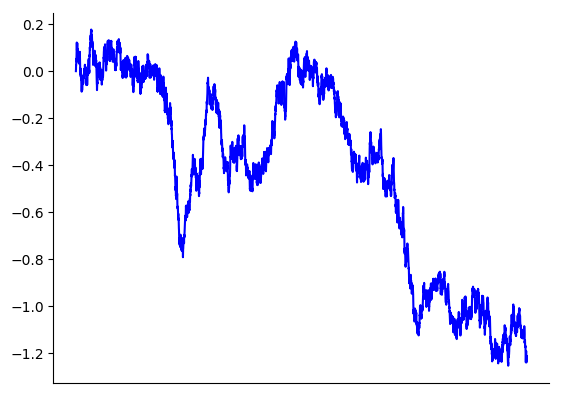
\includegraphics[width=.9\linewidth]{2-brownianb.png}
	\end{subfigure}
	\caption{Three graphs of Brownian motion, a 2-stable L\'evy process.}
	\label{fig:brownian}
\end{figure}



\begin{figure}[h]
	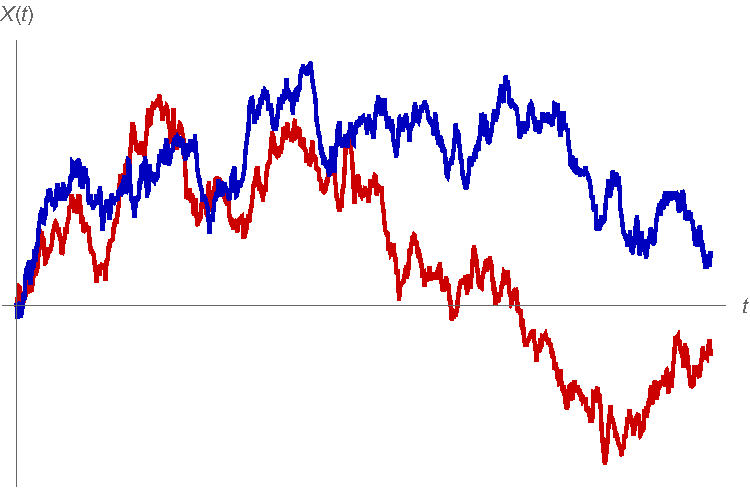
\includegraphics[width=0.5\textwidth]{wiener_process.pdf}
	\caption{\label{fig:brownianmotion}Two graphs of one-dimensional Brownian motion}
\end{figure}

The geometric properties, such as dimension, of Wiener processes have been a particularly well studied area. This includes studying the \emph{graphs}, level sets and \emph{trails} of such processes which can often be thought of as fractals as they often display some \emph{statistical self-affinity}. For any left continuous function $X:\mathbb{R}\to\mathbb{R}$, we define the graph of the function by:
\[
G^{I\subset\mathbb{R}}_{X}=\{(t,y)|y=X(t),t\in I\}\cup J,
\]
where $J$ is the union of vertical segments joining the discontinuities. $J$ is well defined because $X$ is right continuous. It is clear that if $X$ is continuous then $J$ is empty. Taylor \cite{Ta} first calculated the Hausdorff dimension of $d$-dimensional Brownian motion $B_d:\mathbb{R}\to\mathbb{R}^d$ where he showed that almost surely
\[
\dim_\text{H} G_{B_1}^{[0,1]} =  \frac{3}{2}         
\]
and for any $d\ge 2$
\[
\dim_\text{H} B_d([0,1]) =  2.
\]
\textcolor{red}{want to include box dimension result here, equality by kenneth's book}


Another generalisation of Brownian motion is \emph{fractional Brownian motion}, first introduced by Mandelbrot and Van Ness \cite{MVN}. Index-$h$ fractional Brownian motion (fBm) on $\mathbb{R}$ with $0<h<1$ is defined to be the stochastic integral 
\[
B_h (t) = c(h)^{-1} \int_{-\infty}^\infty \left(\left( t-x \right)_+^{h-1/2} - (-x)_+^{h-1/2} \right)W(dx)
\]
where W is the Wiener measure, $(x)_+ = \max\{0,x\}$ and $c(h) = \Gamma(h+1/2)$, where $\Gamma$ denotes the gamma function. Equivalently this is a Gaussian random process $B_h(t)$ with:
\begin{itemize}
	\item[1]: $B_h(0)=0$ almost surely.
	\item[2]: For all $t,u>0$, $B_h(t+u)-B_h(t)$ has normal distribution with mean 0 and variance $u^{2h}$ (Gaussian increments).
	\item[3]: For all $t>0$ $\lim_{u\to 0} B_h(t+u)-B_h(t)=0$ in probability (continuity).
\end{itemize}
One can see that when $h=1/2$, $B_{1/2}(t) = B(t)$ is simply Brownian motion. Much progress has been made on the properties of fBm, see for instance \cite{Ad},\cite{Ka} and \cite{Fa2}. Notably it was shown that almost surely, the graph over the unit interval of index-$h$ fBm has Hausdorff dimension $2-h$. 

\begin{figure}[h]
	\centering
	\begin{subfigure}[b]{0.3\textwidth}
		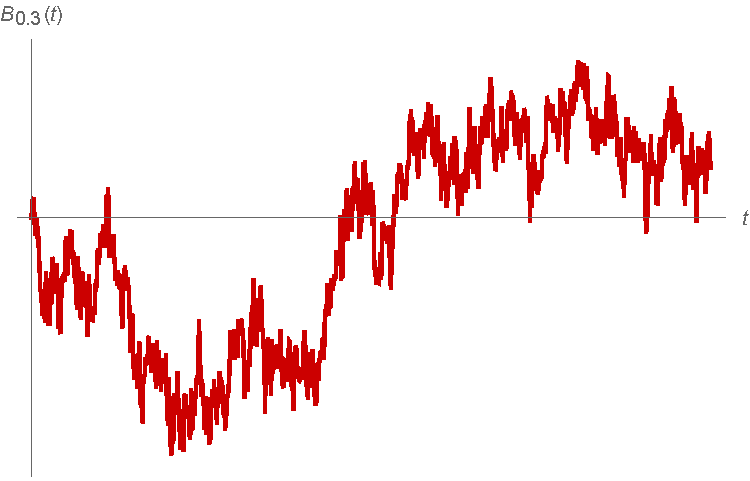
\includegraphics[width=\textwidth]{fbm0_3}
		\caption{Graph of fBm with h=0.3}
		\label{fig:fbm3}
	\end{subfigure}
	~ %add desired spacing between images, e. g. ~, \quad, \qquad, \hfill etc. 
	%(or a blank line to force the subfigure onto a new line)
	\begin{subfigure}[b]{0.3\textwidth}
		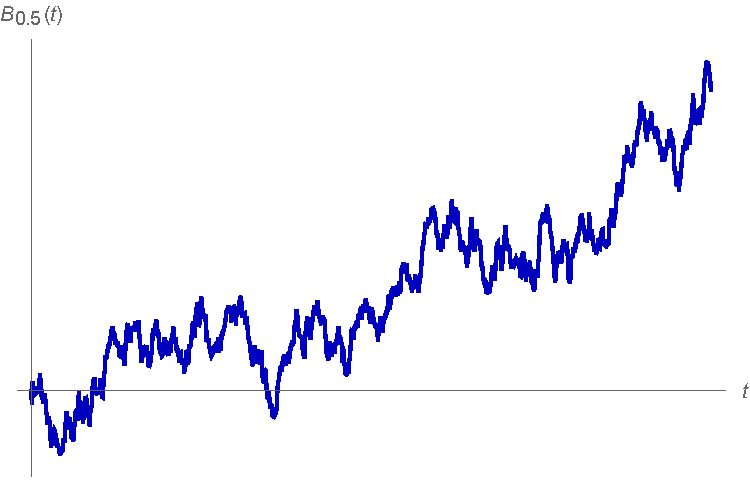
\includegraphics[width=\textwidth]{fbm0_5}
		\caption{Graph of fBm with h=0.5}
		\label{fig:fbm5}
	\end{subfigure}
	~ %add desired spacing between images, e. g. ~, \quad, \qquad, \hfill etc. 
	%(or a blank line to force the subfigure onto a new line)
	\begin{subfigure}[b]{0.3\textwidth}
		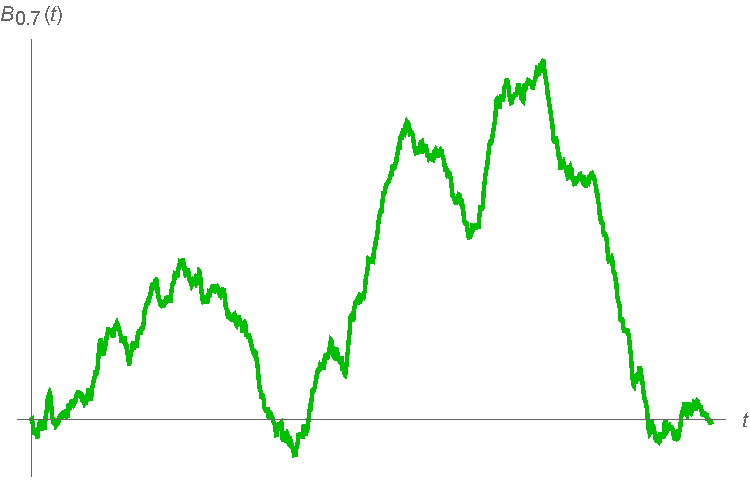
\includegraphics[width=\textwidth]{fbm0_7}
		\caption{Graph of fBm with h=0.7}
		\label{fig:fbm7}
	\end{subfigure}
\end{figure}



Studying the Assouad dimension of various fractals and its properties is an increasingly popular area of research. In this paper, we are interested in calculating the Assouad dimension of the graph $G_X^{[0,1]}$ for $\beta$-scaling (or L\'{e}vy $\beta$-stable) processes and stochastic integrals $X$. These results will be compared to the previously obtained Hausdorff dimensions.

We say that $X(t)$ satisfies a $\beta$-scaling property if, for any $t,a>0$:
\[
a^{-\frac{1}{\beta}}X(at)=^d X(t),
\]
where `$=^d$' denotes `equal in distribution'.
For example the Wiener process has the $2$-scaling property.
The Assouad dimension provides information on the extremal local scaling of a set, in this setting it will tell us about the maximal fluctuations of a random process. For a more detailed introduction to this dimension, see \cite{Fr, Ro}. 

\textcolor{red}{reconfigure whole chapter} This paper will be split into three parts. First we will define a condition, Definition 2.1 which guarantees that a graph will have full Assouad dimension. Then in Section 3 we show that graphs of $\beta$-scaling L\'evy process satisfy this condition and combining these results we prove that graphs of functions defined by certain stochastic integrals also have full Assouad dimension. Finally in Section 4 we remark that our results extend to higher dimensions.

\section{Assouad dimension of graphs}
In this section we will state a convenient condition to check whether a graph of a function $f:[0,1]\to\mathbb{R}$ has full Assouad dimension.

We begin with a definition:

\begin{definition}\label{Win}
	Let $R_1,R_2>0$ be positive numbers and $n_1,n_2>0$ be integers. Given a point $a\in\mathbb{R}^2$, we define $W_{n_1\times n_2}^{R_1\times R_2}(a)$ as the following collection of sets:
	\[	
	\left\{D_{i,j}+a \, \vert \, D_{i,j}=\left[\frac{i}{n_1}R_1,\frac{i+1}{n_1}R_1\right]\times \left[\frac{j}{n_2}R_2,\frac{j+1}{n_2}R_2\right], i\in\{0,\dots,n_1-1\}, j\in\{0,\dots,n_2-1\}\right\}.
	\]
	
	We see that $W_{n_1\times n_2}^{R_1\times R_2}(a)$ is the collection of rectangles with disjoint interiors which partitions the $R_1\times R_2$ rectangle whose bottom left vertex is $a$.
	
	Then let $N_{n_1\times n_2}^{R_1 \times R_2 }(a,G_f^{[0,1]})= \# \left\{ W_{n_1\times n_2}^{R_1\times R_2}(a) \cap G_f^{[0,1]} \right\}$, this is the number of rectangles which intersect the graph.
\end{definition}

The following theorem is a direct consequence of the definition of Assouad dimension and we omit the proof:


\begin{theorem}\label{graph}
	If there exists an $A>0$ and sequences:
	\[
	a_i\in \mathbb{R}^2,R_i\in (0,1),\, n_i\in\mathbb{N} \quad (\forall i\in \mathbb{N})
	\]
	with $n_i \rightarrow \infty$ such that for all $i\in\mathbb{N}$
	\[
	N_{n_i\times n_i}^{R_i \times R_i }(a_i,G_f^{[0,1]})\geq A n_i^2.
	\]
	Then
	\[
	\Assouad G_f^{[0,1]}=2.
	\]
\end{theorem}

Whilst this might seem like a restrictive condition to ask a general function to satisfy, it is quite natural in the setting of Wiener processes due to the almost sure unbounded variation and $\beta$-scaling property of the process. Considering squares instead of balls in the definition of Assouad dimension is similar to the definition of the Furstenberg star dimension, which is in fact equivalent to the Assouad dimenion, see \cite{chenwuwu}.

\begin{remark}
	Note that one could replace the inequality with the following equality
	\[
	N_{n_i\times n_i}^{R_i \times R_i }(a_i,G_f^{[0,1]})= n_i^2.
	\]
	This follows from \cite[Theorem 2.4]{FY}, where it is shown that a set has full Assouad dimension if and only if it has the unit ball as a weak tangent. This means that any cover of our set is also a cover of a ball and so all smaller squares are needed in the cover.
\end{remark}

\section{Applications to  $\beta$-scaling L\'evy processes}\label{LP}

Let $X(t)$ be a L\'evy process. We assume that $X(1)$ is non-vanishing almost everywhere on $\mathbb{R}$ as a random variable, that is, the distribution function of $X(1)$ is 0 only on a set of measure 0. 

Then for any $\beta$-scaling L\'evy process $X$ we can compute the probability of the following event `$N_{n\times n}^{1 \times 1 }(0,G_X^{[0,1]})=n^2$'. It is a positive number depending only on $n$ and we use $P(n)$ to denote this number. The event `$X$ hits a rectangle' is measurable when $X$ is continuous; when it is discontinuous we join the graph with a vertical line and the process is c\`adl\`ag so the event `$X$ hits a rectangle' is still measurable. Thus our event is measurable as the union of measurable events.

For a $\beta$-scaling random process $X$, we can decompose the graph into countably many disjoint parts:
\[
G_X^{[0,1]}=\bigcup_{i=0}^\infty G_X^{I_i},
\]
where $I_i$ are closed intervals with disjoint interiors such that their union is the unit interval. For our case one could think of this as partitioning the unit interval by intervals of length $1/2^i$. For example take $a_1=0$ and for all $i\geq 1$ let $a_{i+1}=a_i+1/2^i$ and $I_i=[a_i,a_i+1/2^{i}].$

Denote by $|I_i|$ the length of interval $I_i=[a_i,b_i]$. Because we can take $X$ as a left continuous function, $X(a_i)\in\mathbb{R}$ is defined for all $i$. For each $i$ we can apply a linear map $T_i: G_X^{I_i} \rightarrow [0,1]^2$:
\[
T_i(x,y)=\left(\frac{1}{|I_i|}(x-a_i),\frac{1}{|I_i|^{1/\beta}}(y-X(a_i))\right).
\]

By definition, it is easy to see that $T_i(G_X^{I_i})$ are independent $\beta$-scaling L\'evy processes with the same, original distribution. For convenience we identify $T_i(G_X^{I_i})=G_{X_i}^{[0,1]}$ where $X_i$  are independent, identically distributed $\beta$-scaling L\'evy processes.

Let $n_i$ be a sequence of integers such that $\lim_{i\to\infty} n_i=\infty$. We can compute the probability of the event $A_i=`N_{n_i\times n_i}^{1 \times 1 }((0,0),G_{X_i}^{[0,1]})=n_i^2 $'. According to the discussions above, we see that the probability is $P(n_i)$. In fact denote $t_k=k/n^2_i$ for all $k\in\{1,\dots,n^2_i\}$ and $D(j)=[j/n_i,(j+1)/n_i]$ for all $j\in\{0,\dots, n_i-1\}$ then we can see that:
\[
P(n_i)\geq P\left(\forall k\in\left[1,n^2_i\right], k\in \mathbb{N},X(t_k)\in D\left(\left\{\frac{k}{n_i}\right\}n_i\right)\right)>0.
\]
Here $\{ \cdot \}$ denotes the fractional part function. The last inequality follows from our assumption that $X(1)$ is non-vanishing almost everywhere on $\mathbb{R}$. It is clear that this restraint could be relaxed to non-vanishing on some interval without much effort. The rest follows from the property of independent increments.

We can choose $n_i$ to grow slowly enough such that $\sum_{i}P(n_i)=\infty$. Note that the $R_i$ can be chosen so that each square is disjoint and as L\'evy processes are Markov, the events $A_i$ are all independent. Then by Borel-Cantelli lemma we see that with probability $1$, infinitely many events $A_i$ occur. Now if $A_i$ happens, then:
\[
N_{n_i\times n_i}^{1 \times 1 }\left((0,0),G_{X_i}^{[0,1]}\right)=n_i^2,
\]
applying the function $T^{-1}_i$ to the graph, we see that (remember $I_i=[a_i,b_i]$):
\[
N_{n_i\times n_i}^{|I_i| \times |I_i|^{1/\beta} }\left((a_i,X(a_i)),G_{X}^{I_i}\right)=n_i^2.
\]

Since $\beta\geq 1$, we see that $|I_i|\leq |I_i|^{1/\beta}$. Also remember that $X$ can be taken to be a right continuous function and we also include the vertical segments of the jumps in $G^{[0,1]}_X$. Therefore it is clear that there exist an absolute constant $C>0$:
\[
N\left(B\left(\left(a_i,X(a_i)\right),|I_i|\right)\cap G_X^{[0,1]},\frac{|I_i|}{n_i}\right)\geq C n_i^2.
\] 

As infinitely many $A_i$ occur, using Theorem \ref{graph}, we see:
\[
\Assouad G_{X}^{[0,1]}=2.
\]

We conclude the above argument as the following theorem:
\begin{theorem}\label{Main}
	Let $X$ be a $\beta$-scaling L\'evy process with $\beta\geq 1$, such that $X(1)$ is a random variable whose distribution function is non-vanishing almost everywhere. Then almost surely:
	\[
	\Assouad G_{X}^{[0,1]}=2.
	\]
\end{theorem}

We know that the Wiener process $W(t)$ is a $2$-scaling L\'evy process, therefore we see that:
\begin{corollary}
	\[
	\Assouad G_{W}^{[0,1]}=2.
	\]
\end{corollary}

Ville Suomala and Changhao Chen, in a personal communication, kindly remarked that this result follows from the graph of Brownian motion having full lower porosity dimension. This approach is inspired by \cite{coxgriffin}, where it was shown that the graph of Brownian motion has full upper porosity dimension. However this porosity dimension technique does not extend to our following, more general result.

In fact we can say more about the Assouad dimension of random processes which are functions defined as stochastic integrals, such as fractal Brownian motion. 

\begin{theorem}
	Let $f:\mathbb{R}\to\mathbb{R}$ be a function which is zero only finitely often, continuous on some interval and has continuous derivative on that same interval. Then we define $B_f(t)$ as the function defined by the stochastic integral:
	\[	
	B_f(t)=\int_0^t f(x) W(dx).
	\]
	We have that almost surely:
	\[
	\Assouad G_{B_f}^{[0,1]}=2.
	\]
\end{theorem}
\begin{remark}
	In particular, graphs of fractional Brownian motions with indices $0<h<1$ have full Assouad dimension almost surely.
\end{remark}
\begin{proof}
	Given a function $f$ which is zero only finitely often, continuous and has continuous derivative on some interval, say $J$, we can simply focus on the function restricted to $J$, normalising to obtain a function which is $C^1$ and zero only finitely often on the unit interval. We may then assume that $f(t)>1$ for $t\in [0,1]$ by again restricting our function to an interval where the function is bounded away from zero and normalising. 
	
	As the Assouad dimension provides local information, if the dimension of the graph of the function defined by stochastic integral of this new function is full then the dimension of the original graph is also full. Thus we assume for the rest of this proof that $f$ is a $C^1$ function which is greater than $1$.
	
	Ideally we would wish to integrate by parts in the standard Riemann–-Stieltjes sense
	\[
	\int_{0}^{t}f(x)W(dx)=f(t)W(t)-\int_{0}^{t}W(x)f'(x)dx.\tag{*}
	\]
	The problem is that the integral on the left side of the above equation is interpreted as the It\^{o} integral, for which regular integration by parts does not hold. There is however a generalisation of this formula for stochastic integrals which holds as $f$ and $W$ are both semimartingales, see \cite{Pr}[Chapter 2 Section 6] for further details. To be precise we should write the following equation
	\[
	\int_{0}^{t}f(x)W(dx)=f(t)W(t)-\int_{0}^{t}W(x)f'(x)dx-[f,W]_t.
	\]
	Here $[f,W]_t$ is the quadratic covariation between $f$ and $W$:
	
	Let $0=t_1<t_2<\dots<t_n=t$ be a partition $P$ of $[0,t]$ and $\vert P \vert$ be the maximum of $t_{k+1}-t_k,k\in\{0,\dots,n-1\}$:
	\[
	[f,W]_t=\lim_{\vert P\vert\to 0} \sum_{i=1}^{n-1} (f(t_{i+1})-f(t_{i}))(W(t_{i+1})-W(t_i)).
	\]
	The above convergence is taken in the sense of probability. By using Cauchy-Schwarz we see that:
	\[
	[f,W]_t\leq [f,f]^{1/2}_t[W,W]^{1/2}_t.
	\]
	However, it is standard that $[f,f]_t=0$ and $[W,W]_t=t$ as $f$ is $C^1$. So we see that the integral by parts formula (*) is indeed correct for this situation. The integral 
	\[
	\int_0^{t} W(x)f'(x)dx
	\]
	is defined to be a random process whose sample space is that of the Wiener process, where fixing a sample path of the Wiener process will determine the integral. We are interested in almost sure properties of this process and will do so by considering almost sure properties of the Wiener process.
	
	The strategy for the rest of this proof is to choose carefully a typical path of the Wiener process. We denote the sample space of the Wiener process as $\Omega$.
	
	First, we see that for almost all $\omega\in\Omega$, $W(t,\omega)$ is c\`adl\`ag in $t$, and therefore there is a constant $C_\omega$ such that:
	\[
	|W(t,\omega)|\leq C_\omega
	\]
	for all $t\in [0,1]$. 
	
	The second almost sure property is described in the proof of Theorem \ref{Main}, that there are infinitely many intervals $I_i=[a_i,b_i]\subset [0,1]$ and a sequence $n_i\to\infty$ such that for $k\in\{0,1,\dots,n_i-1\}$
	\[
	\left|W\left(a_i+(k+1)\frac{|I_i|}{n_i},\omega\right)-W\left(a_i+k\frac{|I_i|}{n_i},\omega\right)\right|\geq |I_i|^{1/2}\geq |I_i|.
	\]
	
	In the following discussion we shall fix a typical $\omega$ such that $W(t,\omega)$ satisfies the above two almost sure properties, in particular, we think of $C_\omega>0$ as a fixed constant.
	
	Then we see that:
	\begin{eqnarray*}
		& &\left|B_f\left(a_i+(k+1)\frac{|I_i|}{n_i},\omega\right)-B_f\left(a_i+k\frac{|I_i|}{n_i},\omega\right)\right|\\
		&=& \left| \int_{a_i+k\frac{|I_i|}{n_i}}^{a_i+(k+1)\frac{|I_i|}{n_i}} f(x)W(dx)\right|\\
		&=& \left| f\left(a_i+k\frac{|I_i|}{n_i}\right)W(x,\omega)\bigg\vert_{a_i+k\frac{|I_i|}{n_i}}^{a_i+(k+1)\frac{|I_i|}{n_i}} + \int_{a_i+k\frac{|I_i|}{n_i}}^{a_i+(k+1)\frac{|I_i|}{n_i}} W(x)f'(x)dx \right|.
	\end{eqnarray*}
	
	Since $f$ is $C^1$, we see that there is a constant $C_f$ (which does not depend on $i$) such that for all $x\in \left[{a_i+k\frac{|I_i|}{n_i}},{a_i+(k+1)\frac{|I_i|}{n_i}}\right]$:
	\[
	\left\vert W(x)f'(x)\right\vert \leq C_f C_\omega.
	\]
	
	Then we have the following inequalities:
	\[
	\left| f\left(a_i+k\frac{|I_i|}{n_i}\right)W(x,\omega)\bigg\vert_{a_i+k\frac{|I_i|}{n_i}}^{a_i+(k+1)\frac{|I_i|}{n_i}} \right| \geq \left| f\left(a_i+k\frac{|I_i|}{n_i}\right) \right| |I_i|^{1/2}\geq |I_i|^{1/2}.\tag{**}
	\]
	and
	\[
	\left\vert\int_{a_i+k\frac{|I_i|}{n_i}}^{a_i+(k+1)\frac{|I_i|}{n_i}} W(x)f'(x)dx \right\vert\leq C_fC_\omega\frac{|I_i|}{n_i}.
	\]
	Since $|I_i|\to 0$,  we see that for a constant $C'$ which depends only on $f$ and $\omega$:
	\[
	\left|B_f\left(a_i+(k+1)\frac{|I_i|}{n_i},\omega\right)-B_f\left(a_i+k\frac{|I_i|}{n_i},\omega\right)\right|\geq C'|I_i|.\tag{***}
	\]
	The above inequality holds for all $k\in\{0,\dots,n_i-1\}$. 
	
	Moreover, $W$ has a `zigzag' property. For even integers $k$ we have
	\[
	W\left(a_i+(k+1)\frac{|I_i|}{n_i},\omega\right)-W\left(a_i+k\frac{|I_i|}{n_i},\omega\right)>0,
	\] 
	for odd integers $k$ we have
	\[
	W\left(a_i+(k+1)\frac{|I_i|}{n_i},\omega\right)-W\left(a_i+k\frac{|I_i|}{n_i},\omega\right)<0.
	\]  
	Heuristically this says that the process increases on the first interval, decreases on the second and so forth, zigzagging from top to bottom. We can see that the expressions inside the absolute values in (**) and (***) also satisfy similar `zigzag' properties. Therefore there is a constant $A=A(\omega,f)>0$ such that:
	\[
	N\left(B\left(\left(a_i,B_f(a_i)\right),|I_i|\right)\cap G_{B_f}^{[0,1]},\frac{|I_i|}{n_i}\right)\geq A n_i^2.
	\] 
	
	This concludes the proof because the above argument holds for a set of full probability $\omega\in\Omega$.
\end{proof}



\section{A remark on higher dimensional Brownian motion}

Definition \ref{Win} has a natural generalization in $\mathbb{R}^d$.
\begin{definition}\label{Win2}
	Let $R_1,\dots,R_d>0$ be positive numbers and $n_1,\dots, n_d$ be integers. Given a point $a\in\mathbb{R}^d$, we define $W_{n_1\times\dots\times n_d}^{R_1\times\dots\times R_d}(a)$ as the following collection of sets:
	\begin{eqnarray*}
		\Bigg\{D_{i_1,\dots,i_d}+a \, \vert \, D_{i_1,\dots,i_d}=\left[\frac{i_1}{n_1}R_1,\frac{i_1+1}{n_1}R_1\right]\times\dots\times \left[\frac{i_d}{n_d}R_d,\frac{i_d+1}{n_d}R_d\right],\\ i_j\in\{0,\dots,n_j-1\}, j\in\{1,\dots,d\}\Bigg\}.
	\end{eqnarray*}
	
	We see that $W_{n_1\times n_2}^{R_1\times R_2}(a)$ is a collection of rectangles with disjoint interiors.
\end{definition}

Using the above definition and a similar argument as the one in section \ref{LP},  Theorem \ref{graph} also extends to higher dimensions, we can show the following result and we omit the proof:

\begin{theorem}
	Let $B_d(t)$ be the $d$ dimensional Brownian motion, from $\mathbb{R}$ to $\mathbb{R}^d$. Then almost surely:
	\[
	\Assouad B_d([0,1])=d.
	\]
\end{theorem}

We can compare this result to the well known \[\dim_{\mathrm{H}} B_d([0,1])=2\] for $d\geq 2$. The Hausdorff dimension being 2 here can be thought as a reflection that higher dimensional Brownian motion is transient, whilst the Assouad dimension shows that there are still areas of maximal fluctuation. 

Brownian motion also provides examples of Salem sets that can have different Hausdorff and Assouad dimensions, we refer the reader to \cite{Ka}  for further discussion on the links between random processes and Salem sets.




\textcolor{red}{do lower dim here}


\textcolor{red}{got some notation to fix wrt previous sections}
\subsection{Pushforwards of measures onto graphs of Brownian motion}


We now turn our attention to pushforwards of measures and ask if doubling and uniform perfectness are preserved in these situations. Specifically we will consider maps from the unit interval onto graphs of L\'evy processes.


Recall the definition of the graph of a L\'evy process $X$ restricted to the unit interval:
\[
G_X^{[0,1]} = \left\{ (t,X(t)) \colon t \in [0,1] \right\}.
\]
More generally, denote by $G_X^I$ the graph of the process $X$ restricted to the interval $I \subseteq [0,1]$. There is a naturally associated map $f: [0,1] \rightarrow \mathbb{R}^2$ which maps the unit interval to the graph of the process, that is $f\colon t \mapsto (t,X(t))$. This will be the map we wish to use to construct pushforward measures, and for the rest of this section $f$ should be assumed to be this map. 

One of the interesting features of L\'evy processes is their statistical self-affinity. Not all processes have this property so we will restrict to \textit{stable} or $\alpha$-\textit{stable processes}, that is for some $\alpha > 0$
\[
a^{-1/\alpha}X(at) =^d X(t)
\]
for all $a,t > 0$ and $=^d$ means equal in distribution. For example the Wiener process is 2-stable. In fact all stable processes have $\alpha \in (0,2]$. 

Our final condition is a simple assumption that the distribution $X(1)$ is non-vanishing on $\mathbb{R}$. Non-zero on an interval would also work, this is just to ensure the graphs are not just multiple flat lines, such as in a Poisson process.


\begin{figure}[htbp]
	\centering
	\begin{subfigure}{0.3\textwidth}
		\centering
		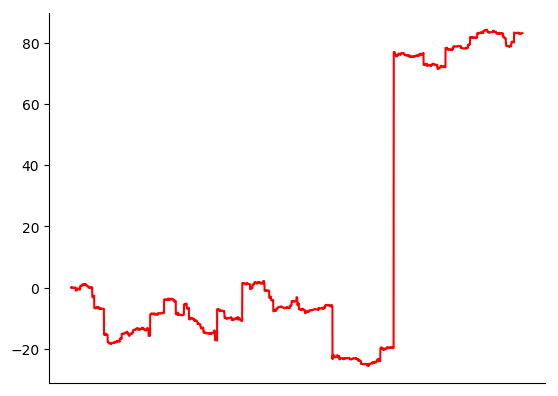
\includegraphics[width=0.85\linewidth]{1-cauchyr.png}
	\end{subfigure}%
	\begin{subfigure}{.3\textwidth}
		\centering
		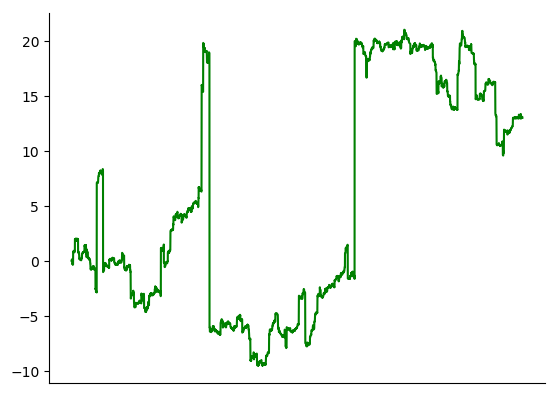
\includegraphics[width=.9\linewidth]{1-cauchyg.png}
	\end{subfigure}%
	\begin{subfigure}{.3\textwidth}
		\centering
		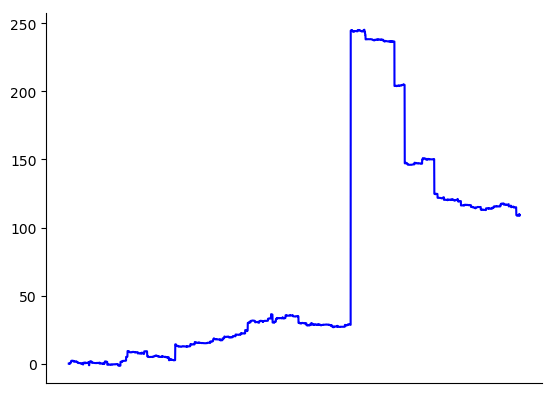
\includegraphics[width=.9\linewidth]{1-cauchyb.png}
	\end{subfigure}
	\caption{Three graphs of a L\'evy process whose increments are Cauchy distributed, a 1-stable L\'evy process.}
	\label{fig:cauchy}
\end{figure}


This leads us to the question of this section: given a doubling measure $\mu$ on the unit interval, is $f_*\mu$ also doubling? A similar question holds for uniformly perfect measures. In \cite{howroyd-yu}, it was shown that the Assouad dimension of $G_X^{[0,1]}$ is almost surely 2 so there must exist at least one doubling measure on the graph. However, most measures on the graph might not even be doubling. For the Hausdorff dimension, the proof by Taylor shows that the Hausdorff dimension of the pushforward of Lebesgue measure almost surely attains the dimension of the graph itself. It turns out that this is usually not the case for the regularity dimensions.

\begin{theorem}\label{brownianthm}
	Let $\mu$ be a doubling measure on $[0,1]$ and $X$ a stable L\'evy process with the distribution $X(1)$ being non vanishing on $\mathbb{R}$. Then $f_*\mu$ is almost surely not doubling on $G_X^{[0,1]}$. Also, $f_*\mu$ is almost surely not uniformly perfect.
\end{theorem}


Trivially this implies the upper regularity dimension of $f_*\mu$ is almost surely infinity and the lower dimension is almost surely zero. Therefore any measure whose upper regularity dimension approximates the dimension of the graph is highly dependent on the specific graph and so there is no one measure that attains the dimension for typical realisations, unlike the Hausdorff case. 


\begin{proof}
    Proof starts here
\end{proof}

Choose a L\'evy process $X$ which satisfies the conditions in Theorem \ref{brownianthm} with scaling coefficient $\alpha$ and fix a graph $G_X^{[0,1]}$ realised by this process. Start by assuming $\alpha > 1$, the proof will work in the same way for $\alpha < 1$ given a slight modification which will be commented on later in the proof. $\mu$ is taken to be a doubling measure on the unit interval. Recall $f$ is defined to be the function which maps the unit interval to the graph of our L\'evy process and $f_*\mu$ is the pushforward measure of $\mu$ onto the graph that we wish to study. \textcolor{red}{properly explain difference when $\alpha < 1$}

We start by calculating the almost sure upper regularity dimension of $f_*\mu$. Let $s>0$. The general strategy for this proof is to find a sequence of events that are all independent and have positive probability. Then a simple application of the Borel-Cantelli lemma will yield that almost surely these events will happen infinitely often. By choosing our events carefully this will yield a sequence of balls that show the upper regularity dimension of the pushforward measure must be greater than $s$. As $s$ is abitrary, this will conclude the proof.

Given our $\alpha$-scaling L\'evy process, we define the rectangle centered at $a\in [0,1]$ with side lengths $R_1,R_2$ by $Rec(a,R_1,R_2) = I(a,R_1) \times I(X(a),R_2)$ where $I(b,R) = [b-R/2,b+R/2]$ is just an interval of length $R$ and centre $b$. $G_X^{I(x,R)}$ will denote the graph of $X$ above the interval $I(x,R)$.

The particular events $E_i$ we are interested in are defined as follows: let $x_i \in [0,1]$, $R_i > r_i> 0$ and $\beta > 1$, then $E_i$ is the event in which $G_X^{I(x_i,R_i^{\alpha})} \subset Rec(x_i,R_i^{\alpha},R_i)$ and $Rec(x_i, r_i, r_i^{1/\alpha}) \cap G_X^{I(x_i,r_i)} = G_X^{I(x_i,r_i^{\beta})}$. These events are chosen so that the measure on the graph will be `large' on the rectangle of small side length $R^{\alpha}$ but `small' on the rectangle of small side length $r$. Figure \ref{brownian_event} is a geometric representation of such an event.  

\begin{figure}[htbp]
	\centering
	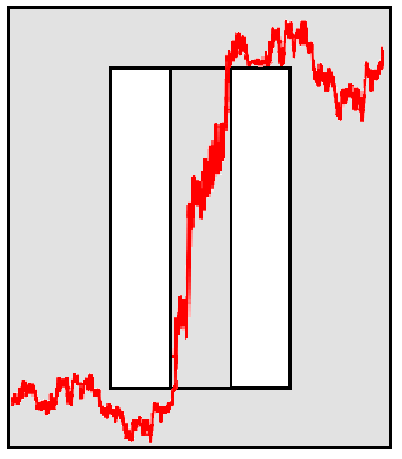
\includegraphics[width=0.4\textwidth]{new_rectangles.png}
	\caption{Example of an event $E_i$, the grey areas are where the graph intersects the rectangles whilst the graph will not intersect the white areas. An example of a graph satisfying this event is in red.}
	\label{brownian_event}
\end{figure}


Note that $\alpha>1$ here is important for the rectangles to be tall and thin. If $\alpha < 1$ it would suffice to change $Rec(x_i,R_i^{\alpha}, R_i)$ to $Rec(x_i, R_i, R^{\alpha})$ and similarly for the smaller rectangles. The rest of the proof would run in the same way afterwards with some slight changes in the calculations of $\beta$ at the end.

Given any sequences $x_i \in [0,1]$, $R_i > r_i > 0$ and $\beta > 1$ we can consider the associated events $E_i$ as above. To make sure the `smaller' rectangle is actually smaller, assume $R_i^{\alpha} > r_i$ without loss of generality. If $Rec(x_m,R_m^{\alpha}, R_m) \cap Rec(x_n,R_n^{\alpha},R_n) = \emptyset$ for all $m\neq n$, then the events are all independent due to the independent increment property of the L\'evy process. As long as the distribution of $X(1)$ is non-vanishing on the unit interval, the probability of any of these events is positive.

We can now choose our sequence of events. Start by picking any disjoint and strictly increasing sequence of reals  $x_i$, $\left\{1-2^{-i} \right\}_{\mathbb{N}}$ would suffice. Then the $R_i$ are taken so that the intervals $I(x_i, R_i)$ do not overlap ensuring independence, say $4^{-i}$. Initially any sequence of $r_i$ can be chosen as long as $R_i/r_i \rightarrow \infty$ and, again, $R_i^{\alpha} > r_i$ for each $i$. $\beta$ will be fixed later, for now it is just a real greater than 1. As the process is $\alpha$-scaling one can map $Rec(x_i,R_i^{\alpha},R_i)$ onto the unit square via an affine map $T$ and the image of the graph under this transformation, denoted $G_{X_i}^{[0,1]}$, will have distribution $X_i$ equal to the original distribution $X(t)$ as it is scaled following the definition of $\alpha$-scaling, so $X(t) = X(R_i^\alpha t)/R_i = X_i(t)$ in distribution. Therefore the probability of an event $E_i$ is equal to the probability the graph of $X_i$ stays in the unit square and 
$$Rec(1/2,r_i/R_i^{\alpha} ,r_i^{1/\alpha}/R_i ) \cap G_{X_i}^{I(1/2, r_i/R_i^{\alpha})} = G_{X_i}^{I(1/2, r_i^{\beta}/R_i^{\alpha})}.$$

Thus the probability of $E_i$ depends solely on the ratio $R_i/r_i = q_i$. If $\sum P(E_i)$ diverges then the conditions for Borel-Cantelli are satisfied and the argument continues. However, if not, the sequence $r_i$ is modified in the following way. Each $i$ gives us a ratio $q_i$ and a probability $P(E_i)$. Construct a function $g \colon \mathbb{N} \rightarrow \mathbb{N}$ such that $g(n) = \lceil \frac{1}{nP(E_n)}\rceil$ for all $n\in \mathbb{N}$. Then, keeping $R_i$ fixed, change the $r_i$ so that each ratio $q_i$ is repeated $g(i)$ many times. For instance, if $g(1) = 3$ then $r_1,r_2$ and $r_3$ are chosen so that $R_1/r_1, R_2/r_2$ and $R_3/r_3$ all give the same $P(E_1)$ and $r_4$ then is chosen with respect to $P(E_2)$ etc. The new sequence is constructed such that $\sum P(E_i)$ diverges, satisfying the conditions for Borel-Cantelli.

Hence, by the Borel-Cantelli lemma, infinitely many $E_i$ occur with probability one. So there are sequences $x_i \in [0,1]$, $R_i > r_i > 0$ and $\beta > 1$ such that, with full probability, all of the events $E_i$ happen and $R_i/r_i \rightarrow \infty$. 

Given a specific event $E_i$ we wish to consider the measure of the rectangles. The ratio of measures of such rectangles is determined by the original measure on the interval. We let $t = \lrdim \mu / 2$, this is just to have a number for which the following bound holds but is also fixed and positive due to Proposition 2.1. Thus we obtain the following bound:
\[
\frac{f_*\mu(Rec(x_i,R_i^{\alpha},R_i))}{f_*\mu(Rec(x_i,r_i,r_i^{1/\alpha}))} = \frac{\mu(B(x_i, R_i^{\alpha}))}{\mu(B(x_i, r_i^{\beta}))} \ge C\left(\frac{R_i^{\alpha}}{r_i^{\beta}}\right)^t, 
\]
where $C$ comes from the definition of the lower regularity dimension.

The only variable left to be fixed is $\beta$. We wish to have the above ratio greater than $C(R_i/r_i)^s$. After a short calculation, it is clear that this is always true if $\beta \ge \alpha + s/t$. Thus by choosing such a $\beta$ we have
\[
\frac{f_*\mu(Rec(x_i,R_i^{\alpha},R_i))}{f_*\mu(Rec(x_i,r_i,r_i^{1/\alpha}))} \ge C\left(\frac{R_i^{\alpha t}}{r_i^{\alpha t + s} }\right) \ge C\left(\frac{R_i^{\alpha t + s}}{r_i^{\alpha t + s} }\right)  \ge
C\left(\frac{R_i}{r_i}\right)^s. 
\]

To show the upper regularity dimension is greater than $s$ we need to consider balls not rectangles. Thankfully due to our construction $B(x_i,R_i) \supset Rec(x_i, R_i^\alpha, R_i)$ and $B(x_i,r_i) \subseteq Rec(x_i, r_i, r_i^{1/\alpha})$. Hence
\[
\frac{f_*\mu(B(x_i,R_i))}{f_*\mu(B(x_i,r_i))} \ge \frac{f_*\mu(Rec(x_i,R_i^{\alpha},R_i))}{f_*\mu(Rec(x_i,r_i,r_i^{1/\alpha}))} \ge C\left(\frac{R_i}{r_i}\right)^s ,
\]
completing the proof.


For the lower regularity dimension it suffices to change the events $E_i$ in the following way. Assuming $\alpha>1$, let $x_i \in [0,1]$, $R_i > r_i > 0$ and $\beta < 1$, then $E_i$ is the event where $G_X^{I(x_i, R_i)} \cap Rec(x_i,R_i,R_i^{1/\alpha}) \subseteq Rec(x_i, r_i^{\beta}, R_i^{1/\alpha})$ and $G_X^{I(x_i, r_i)} \subseteq Rec(x_i, r_i^{\alpha}, r_i)$. The previous argument then works in much the same way, showing that the lower regularity dimension of $f_*\mu$ is zero as desired.

\begin{figure}[htbp]
	\centering
	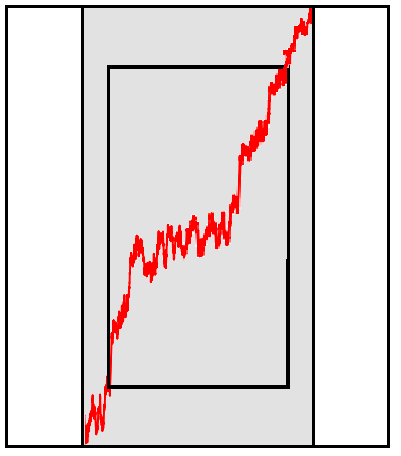
\includegraphics[width=0.4\textwidth]{rectangles.png}
	\caption{Example of an event $E_i$ for the lower regularity dimension, the grey areas are where the graph intersects the rectangles whilst the graph will not intersect the white areas.}
	\label{brownian_event}
\end{figure}







\chapter{Open Problems}
\label{chap:conclusion}



To conclude this thesis, we will recall and expand upon some of the questions that have been raised so far. This will merely be a list of problems that we found interesting when writing this work and is in no way exhaustive, but should offer a number of options for future work. In this chapter we will follow the general order in which the work was presented in this thesis without recalling specific notation that was introduced previously.


\section{Weak tangent measures}\label{ch-conclusion:weak-tangents}

In Chapter 2 we introduced the concept of weak tangent measures and Theorem \ref{ch-upper-reg:weaktangents} showed that the upper regularity dimension of a measure is bounded below by the upper regularity dimension of its weak tangent measures. This is a natural analogue of the set theoretic setting, where weak tangent sets have Assouad dimension less than or equal to the Assouad dimension of the original set. Recently, in \cite{microsets}, it was shown that for any $\mathcal{F}_{\sigma}$ set $\Delta \subseteq [0,1]$ which contains its infimum and supremum, there exists a set $F \subseteq [0,1]$ such that the set of all possible Hausdorff dimensions of the weak tangents of $F$ equals $\Delta$. It is natural to ask if the same holds in the measure theoretic setting.

\begin{question}
What set theoretic restrictions are there on the set $\Delta \subseteq (0,\infty)$ which contains its infimum and supremum such that one can find a locally finite, Borel measure $\mu$ supported on a subset of $\mathbb{R}$ so that
\[
\left\{ \underline{\dim}_{\textup{H}} \hat{\mu} \colon \hat{\mu} \textup{ is a weak tangent measure of } \mu \right\} = \Delta ?
\]
\end{question}

Note in the above question it is assumed that the sets $\Delta$ contain their infimum and supremum, this is due to the fact that the Assouad and lower dimensions of a set is always attained by their microsets. It is perhaps reasonable to assume that this also holds for measures but this should be investigated further.

\begin{question}
For any measure $\mu$ supported on $\mathbb{R}$, is it true that there exists a weak tangent measure $\hat{\mu}$ such that 
\[
\urdim \mu = \urdim \hat{\mu}
\]
and another weak tangent measure $\hat{\mu}'$ such that
\[
\lrdim \mu = \lrdim \hat{\mu}' ?
\]
\end{question}



\section{Self-similar and self-affine measures}\label{ch-conclusion:self-similar}

There has been much work calculating the dimensions of self-similar and self-affine sets in a range of different settings. Here we restricted to self-similar measures on sets satisfying the strong separation condition. This is required to ensure these measures are doubling. However, there are still many examples of doubling self-similar measures for which only a weaker separation condition holds, such as the open set condition. Understanding which measures are still doubling when the separation conditions are weakened would be the first step in calculating the regularity dimensions of these measures.

Another strand of research can be found in \cite{hare-hare-tros}, where the quasi-Assouad dimension of self-similar measures was studied. This different notion of dimension only depends on the measure being quasi-doubling, a weaker property than doubling and so only a weaker separation is required for these calculations. The quasi-Assouad dimension is closely related to the upper regularity dimension so it is likely that the ideas in \cite{hare-hare-tros} could be used to further our understanding of the regularity dimensions too. 

For self-similar measures there are a number of different separation conditions with various notions of dimensions and regularity to consider so, for brevity, we simply state this as the following question which can also be found on page 30.

\begin{question}
What are the regularity dimensions of self-similar measures on sets not satisfying the strong separation condition?
\end{question}


After studying self-similar measures it was natural to turn our attention to self-affine measures on Bedford-McMullen sponges. The regularity dimensions were calculated for such measures assuming two conditions - the very strong separation condition and inequality of the contraction ratios. The first was needed to ensure the measures were doubling; as before it would be interesting to ask which, if any, conditions guarantee doubling. The second condition is important in the proof of our theorem and was first remarked upon in \cite{fraser-howroyd1} in the set theoretic setting. This was removed for the Assouad and lower dimensions of sets in \cite{howroyd-sponges} and it seems reasonable that the techniques in that paper can be used in a similar way for the regularity dimensions of measures. 

As noted in Section 2.2.4, there are a number of generalisations of Bedford-McMullen sponges that have been considered in the literature, covering several different notions of dimension. Finding the regularity dimensions of measures in the examples for which the Assouad and lower dimensions have been studied should be possible by combining the measure theoretic techniques used here with the new tools introduced in the set theoretic settings. For the remaining cases, it would be worth turning our attention to the study of the Assouad dimension first, before attempting to find the regularity dimensions. All these problems were resumed on page 35 in the following question.

\begin{question}
What can be said about the regularity dimensions of self-affine measures on sets which do not satisfy the VSSC? What are the regularity dimensions of self-affine measures on more general carpets, such as Lalley-Gatzouras carpets?
\end{question}



\section{Measures on sequences}\label{ch-conclusion:seq}


Sequences have proven to be particularly interesting objects of study with respect to the Assouad dimension in terms of how different the results often are compared to the more common dimensions. The regularity dimensions of measures on sequences have also shown to exhibit similar phenomena and it would be helpful to have further examples at hand to better understand these dimensions. A natural way of obtaining more examples would be to consider different decay rates, such as stretched exponential, to see if the measures remain doubling as long as the decay rates of the sequence and the measure are comparable. 

One could also look at more general sequences, for instance by removing the decreasing gap condition. However, it would be important to maintain some reasonable conditions to ensure the set and measure continue to resemble genuine sequences. How to formalise this idea at the moment is not clear, further study would have to be undertaken to understand when these sequences develop behaviour that we do not consider `normal' for such objects. As this second part is less precise we omit formally stating it as a question for now, simply recalling the problem posed on page 37.

\begin{question}
How does the upper regularity dimension of measures defined on sequences behave for different decay rates, such as stretched exponential decay?
\end{question}



\section{Quantifying doubling and uniform perfectness}\label{ch-conclusion:quant}


In Chapter 3 it was seen that there is a link between the upper regularity dimension and the doubling constants, similarly for the lower analogues. However, this only relies on the limiting behaviour of the doubling constants $C(\theta)$ as $\theta$ tends to infinity and so not does not imply any obvious behaviour for small $\theta$. The following is a natural question to then ask.
\begin{question}
Given $a, b , \theta > 1$, does there exists a measure $\mu$ such that $a = C(\theta)$ and $b = K(\theta)$?
\end{question}  
There are a number of extensions to this question that can be posed, such as replacing $a, b$ and $\theta$ by sequences $a_i,b_i,\theta_i$ and asking one measure to have constants $C(\theta_i) = a_i$ and $K(\theta_i) = b_i$ for all $i$. Or one could keep the question as is but simultaneously impose specific regularity dimensions on the measure. 

Whilst these questions are interesting, it is currently difficult to calculate these optimal constants even in the simple self-similar setting for specific $\theta$. Developing a better understanding of how these constants behave would be the first step in finding an answer. Doing this would also improve our study of the relations between the regularity dimensions and doubling and uniform perfectness. For instance, in Proposition 4 of Chapter 3, we showed that a doubling measure on a uniformly perfect space has not only positive lower regularity dimension, but also a lower bound to this dimension can be stated explicitly in terms of the doubling constant for a specific $\theta$. If a relation between the doubling constants for various values of $\theta$ can be found, then it is plausible that this bound can be improved. 

To start this analysis we state the following problem which should be achievable.

\begin{question}
Given a self-similar set satisfying the OSC and a self-similar measure on this set, what are the optimal constants $C(\theta)$ and $K(\theta)$ for all $\theta > 1$?
\end{question}


\section{Quantifying doubling and uniform perfectness}\label{ch-conclusion:diophantine}

To finish Chapter 3 we showed that the lower regularity dimension can have applications in Diophantine approximation, providing a hopefully more applicable version of a Theorem in \cite{beres-sanju-al} as the regularity dimensions have now been calculated for a range of different examples. There have been other studies related to the work of \cite{beres-sanju-al} which rely on different regularity properties of measures and it seems reasonable to ask if and how the upper and lower regularity dimensions interact with these notions. A common condition that occurs in this setting is that the measure be `locally doubling'. This lends credibility to the idea that the upper regularity dimension is also involved in some way. We leave this investigation open by recalling the question stated on page 64.

\begin{question}
Is there a relation between the regularity dimensions and other notions of regularity of measures used in Diophantine approximation?
\end{question}


\section{Graphs of Brownian motion}\label{ch-conclusion:brownian}

There are several cases left unresolved in the study of the dimensions of graphs of Brownian motion and measures supported on them. Regarding the Assouad dimension of the graph, it is still not clear what the dimension will be when the $\alpha$-stable L\'evy process has $\alpha < 1$. Following the usual behaviour of the Assouad dimension, it is likely almost surely full but this is not clear in this setting. Any proof would likely need new ideas compared to the ones used in this thesis for the case $\alpha > 1$. The following is a slightly reworded version of the question from page 76.

\begin{question}
For any $\alpha \in (0,1)$, what is the Assouad dimension of the graph of an $\alpha$-stable L\'evy process? 
\end{question}

It would also be natural to consider the lower dimension of the graphs of random process which are functions defined as stochastic integrals. The proof for the Assouad dimension analogue relied heavily on understanding the behaviour of the Wiener process as seen in the calculation of the dimension of the graph of the Wiener process. A similar idea was used for the lower dimension of graphs of L\'evy processes, so it should be possible to combine these ideas and the lower dimension of the graph of stochastic integrals is likely almost surely 1. However, one must be careful in the proof as many of the bounds used for the Assouad dimension do not necessarily hold in the other direction. The question on what the lower dimension actually is was stated on page 77.

\begin{question}
Can a lower dimension analogue of Theorem 8 (from Chapter 3) be found? Given that this result mirrors the Assouad dimension of the graphs of Brownian motion it is natural to conjecture that the lower dimension in this setting will be almost surely 1.
\end{question}




\end{large}


\singlespacing
\printnomenclature
\clearpage
\phantomsection
\onehalfspacing

\singlespacing
\bibliography{bibliography}
%\bibliographystyle{apalike}
\bibliographystyle{alpha-2}



\begin{large}
\chapter*{Appendix}
\addcontentsline{toc}{chapter}{Appendix}

Many of the pictures used in this thesis were created in Mathematica or Python using a simple chaos game algorithm. The below algorithms can be run directly in Mathematica to obtain similar images. Similar Python code is available at https://github.com/douglashowroyd/IFSGen.

The following code can be easily modified to change the output. If a higher quality image is desired then the integer in the first line (currently 10000) should be increased, note that this will proportionally increase the run time and the program might not work if made too high. 

The sections contained within the square brackets following a \textit{Which} define the functions in the IFS. In the higher dimensional versions there is a \textit{Which} for each dimension and each one contains the function's action on a specific coordinate. One can also change the number of functions in the IFS by simply changing the 3 in the first line (4 in the 3-dimensional code) to the desired number of maps and adding the functions to the corresponding \textit{Which} line, for example, in the format  ` j==4, x/5+1/5 ' .

 
 
  \begin{lstlisting}[language=Mathematica,title={Mathematica code for 1-dimensional images}]
    functions=RandomInteger[{1,3},10000];
    
    f[j_,x_] := Which[ j ==1, x/5, j==2, x/5+2/5, j==3, x/5+4/5 ];
    
    sample={0};
    
    For [ i=1, i<=Length[functions], i++, 
    AppendTo[ sample, { f[functions[[i]],sample[[i]], 1 }] 
    ];
    
    ListPlot[ sample, PlotStyle -> PointSize[0.000000001], Axes -> {False,False}]
  \end{lstlisting}
  
  \begin{figure}[htb]
        \centering
        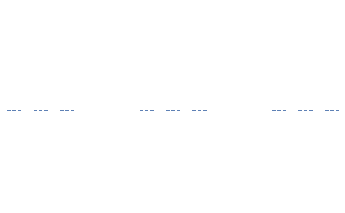
\includegraphics[width=0.3\linewidth]{pics/appendix/1-d_mathematica.png}
        \caption*{The image generated by the above code, here a self-similar set in ambient spatial dimension 1}
    \end{figure}
  
  
  \begin{lstlisting}[language=Mathematica,title={Mathematica code for 2-dimensional images}]
    functions=RandomInteger[{1,3},10000];
    
    f1[j_,x_] := Which[ j ==1, x/2, j==2, x/2, j==3, x/2+1/2 ];
    
    f2[j_,y_] := Which[ j ==1, y/2, j==2, y/2+1/2, j==3, y/2+1/4 ];
    
    sample={{0,0}};
    
    For [ i=1, i<=Length[functions], i++,
    AppendTo[ sample, { f2[functions[[i]],sample[[i]][[1]]],  f1[functions[[i]],sample[[i]][[2]]] }  
    ];
    
    ListPlot[ sample, PlotStyle -> PointSize[0.000000001], AspectRatio -> Automatic, Axes -> {False,False}]
  \end{lstlisting}
  
  \begin{figure}[htb]
        \centering
        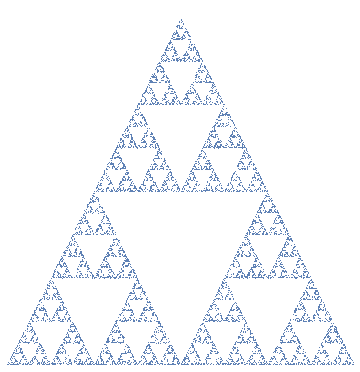
\includegraphics[height=0.5\linewidth]{pics/appendix/2-d_mathematica.png}
        \caption*{The image generated by the above code, here a Sierpi{\'n}ski triangle}
    \end{figure}
  

 
  
  \newpage
  \begin{lstlisting}[language=Mathematica,title={Mathematica code for 3-dimensional images}]
    functions=RandomInteger[{1,4},10000];
    
    f1[j_,x_] :=Which[ j ==1, x/2,
    j==2, x/2,
    j==3, x/2+1/2,
    j==4, x/2+1/4
    ];
    
    f2[j_,y_] := Which[ j ==1, y/2,
    j==2, y/2+1/2,
    j==3, y/2+1/4,            
    j==4, y/2+1/4                   
    ];
    
    f3[j_,z_] := Which[ j ==1, z/2,
    j==2, z/2,
    j==3, z/2 ,                                       
    j==4, z/2+1/2                                                   
    ];
    
    sample={{0,0,0}};
    
    For [ i=1, i<=Length[functions], i++,
    AppendTo[ sample, {
    f1[functions[[i]],sample[[i]][[1]]],  
    f3[functions[[i]],sample[[i]][[2]]],
    f2[functions[[i]],sample[[i]][[3]]]   
    }]
    ];
    
    ListPointPlot3D[ sample, PlotStyle -> PointSize[0.000000001], BoxRatios -> Automatic, Ticks -> None]
  \end{lstlisting}
 
  \begin{figure}[htb]
        \centering
        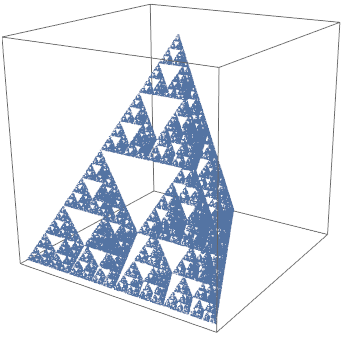
\includegraphics[height=0.5\linewidth]{pics/ch-upper-reg/sierptetra.png}
        \caption*{The image generated by the above code, here a Sierpi{\'n}ski tetrahedron}
  \end{figure}
    
     
\end{large}

\end{document}
